\documentclass{article}
\usepackage{nips_2016}

\usepackage[utf8]{inputenc} % allow utf-8 input
\usepackage[T1]{fontenc}    % use 8-bit T1 fonts
\usepackage{hyperref}       % hyperlinks
\usepackage{url}            % simple URL typesetting
\usepackage{booktabs}       % professional-quality tables
\usepackage{amsfonts}       % blackboard math symbols
\usepackage{nicefrac}       % compact symbols for 1/2, etc.
\usepackage{microtype}      % microtypography

\usepackage{graphicx}
\usepackage{tikz}
\usepackage{amssymb,amsmath}
%\usepackage{natbib}
\DeclareMathOperator*{\argmin}{arg\,min}
\DeclareMathOperator*{\sign}{sign}
\DeclareMathOperator*{\Lik}{Lik}
\DeclareMathOperator*{\Peaks}{Peaks}
\DeclareMathOperator*{\HotSpots}{HotSpots}
\newcommand{\Cost}{\text{Cost}}
\usepackage{stfloats}
\DeclareMathOperator*{\Diag}{Diag}
\DeclareMathOperator*{\TPR}{TPR}
\DeclareMathOperator*{\Segments}{Segments}
\DeclareMathOperator*{\Changes}{Changes}
\DeclareMathOperator*{\FPR}{FPR}
\DeclareMathOperator*{\argmax}{arg\,max}
\DeclareMathOperator*{\maximize}{maximize}
\DeclareMathOperator*{\minimize}{minimize}
\newcommand{\ZZ}{\mathbb Z}
\newcommand{\NN}{\mathbb N}
\newcommand{\RR}{\mathbb R}

\begin{document}

\title{A linear time algorithm for peak detection using constrained
  optimal segmentation}

\author{
  Toby Dylan Hocking\\
  Department of Human Genetics\\
  McGill University\\
  Montreal, QC H2R-2G9 Canada \\
  \texttt{toby.hocking@mail.mcgill.ca} \\
  %% examples of more authors
  \And
  Guillem Rigaill \\
  University of Evry \\
  Evry, France \\
  \texttt{guillem.rigaill@evry.fr} \\
  %% \AND
  %% Coauthor \\
  %% Affiliation \\
  %% Address \\
  %% \texttt{email} \\
  %% \And
  %% Coauthor \\
  %% Affiliation \\
  %% Address \\
  %% \texttt{email} \\
  %% \And
  %% Coauthor \\
  %% Affiliation \\
  %% Address \\
  %% \texttt{email} \\
}

\maketitle

\begin{abstract}
  Change-point detection is a central problem in time series and
  genomic data sets. In several kinds of data it is desirable to
  constrain the possible change-points to obtain a more interpretable
  model. We propose a new constrained Pruned Dynamic Programming
  Algorithm (cPDPA) which recovers the optimal change-points subject
  to affine constraints on adjacent segment means. We use this
  algorithm for isotonic regression and peak detection.
\end{abstract}

\section{Introduction}

Change-point detection is a central problem in many fields. TODO ref
isotonic regression and PAVA.

An algorithm with quadratic time complexity was proposed to solve the
peak detection problem \citep{PeakSeg}. 

\citet{pruned-dp} proposed a Pruned Dynamic Programming Algorithm
(PDPA) to exactly solve the unconstrained segmentation problem.

\subsection{Contributions}

The main contribution of this paper is a new Constrained Pruned
Dynamic Programming Algorithm (cPDPA) which is guaranteed to recover
the exact solution for a class of constrained optimal segmentation
problems. 

\section{Related work}
\label{sec:related}

\subsection{Maximum likelihood segmentation models}

The model we consider in this paper is a constrained version of the
optimal segmentation model \citep{TODO_MORE_REFS,Segmentor}. The
unconstrained model can be computed using a dynamic programming
algorithm (DPA) \citep{bellman}, or a pruned dynamic programming
algorithm (pDPA) \citep{pruned-dp}. Both algorithms are guaranteed to
recover the exact solution to the unconstrained model, but there are
two important differences. The pDPA is more complicated to implement,
but is also computationally faster than the DPA. For segmenting a
sequence of $d$ data points, the pDPA takes on average $O(d\log d)$
time whereas the DPA takes $O(d^2)$ time.

The constraints that we consider in this paper are a generalization of
the peak detection model \citep{PeakSeg} and the isotonic regression
model \citep{isotonic}. Rather than searching all possible
change-points to find the most likely model with $s$ segments, we
propose to constrain the possible change-points so that the segment
means may be more easily interpreted.

\section{From unconstrained to constrained maximum likelihoood
  segmentation}
\label{sec:model}

In this section we first discuss the existing unconstrained maximum
likelihood model, and then we discuss a more general framework for
constrained maximum likle

\subsection{Unconstrained maximum likelihood segmentation}

For a sequence of $d$ data points $\mathbf y\in\ZZ_+^d$ to segment, we
fix a maximum number of segments $ s_{\text{\text{max}}}\leq d$. The
unconstrained maximum likelihood segmentation model is defined as the
most likely mean vector $\mathbf m\in\RR^d$ with $s\in\{1, 2, \dots,
s_{\max}\}$ piecewise constant segments:
\begin{align}
  \label{unconstrained}
  \mathbf{\hat m}^s(\mathbf y)  =\ 
  &\argmin_{\mathbf m\in\RR^{d}} && 
  \ell
  %\tag{\textbf{Unconstrained}}
  (\mathbf m, \mathbf y) \\
  &\text{such that} && \Segments(\mathbf m)=s,
  \nonumber
\end{align}
where the loss function is
\begin{equation}\label{eq:loss}
  \ell(\mathbf m, \mathbf y)= \sum_{j=1}^d m_j - y_j \log m_j.
\end{equation} 
The model complexity is the number of piecewise constant segments
\begin{equation}
  \Segments(\mathbf m)=1+\sum_{j=2}^d I(m_j \neq m_{j-1}),
\end{equation}
where $I$ is the indicator function. 

Although it is a non-convex optimization problem, the sequence of
segmentations $\mathbf{\hat m}^1(\mathbf y), \dots, \mathbf{\hat
  m}^{s_{\text{\text{max}}}}(\mathbf y)$ can be computed in
$O(s_{\text{\text{max}}} d^2)$ time using dynamic programming
\citep{bellman}, or in $O(s_{\text{\text{max}}} d \log d)$
time using pruned dynamic programming \citep{pruned-dp, Segmentor}.

We refer to (\ref{unconstrained}) as the ``unconstrained'' model
since $\mathbf{\hat m}^s(\mathbf y)$ is the most likely segmentation
of all possible models with $s$ piecewise constant segments ($s-1$
change-points). Several unconstrained models are shown on the left of
Figure~\ref{fig:Segmentor-PeakSeg}, and for example the second segment
of the model with $s=3$ segments appears to capture the peak in the
data.
% In general, we would like to use the 2nd, 4th,
% ... segments as peaks, and the 1st, 3rd, ... segments as
% background. 
To construct a peak detector $c$, we first define the peak indicator at base
$j\in\{2, \dots, d\}$ as
\begin{equation}
  \label{eq:peaks}
  P_j(\mathbf m) = \sum_{k=2}^j \sign( m_{k} - m_{k-1} ),
\end{equation}
where $P_1(\mathbf m)=0$ by convention. $P_j(\mathbf m)$ is the
cumulative sum of signs of changes up to point $j$ in the piecewise
constant vector $\mathbf m$. We define the vector of peak indicators
as
\begin{equation}
  \mathbf
P[\mathbf m] = \left[\begin{array}{ccc} P_1(\mathbf m) & \cdots &
    P_d(\mathbf m)
\end{array}\right].
\end{equation}

\subsection{PeakSeg: constrained maximum likelihood}
\label{sec:constrained}

In general for the unconstrained model $P_j(\mathbf m)\in\ZZ$, which
is problematic since we want to use it as a peak detector with binary
outputs $P_j(\mathbf m)\in \{0, 1\}$. 

For example, if $\mathbf m = \left[\begin{array}{ccccccc}1.1 &
    1.1 & 2 & 2 & 4 & 4 & 3\end{array}\right]$, with two changes up
followed by one change down, then $\mathbf P(\mathbf m) =
\left[\begin{array}{ccccccc}0 & 0 & 1 & 1 & 2 & 2 &
    1 \end{array}\right]$.

% This is also a practical problem that can be observed in real data
% sets. For example in Figure~\ref{fig:Segmentor-PeakSeg} there is a position $j$ for
% which $P_j\left[ \mathbf{\hat m}^5(\mathbf y) \right]=2$ (since the
% mean changes up, up, down, down). 

Thus we constrain the peak indicator $P_j(\mathbf
m)\in\{0, 1\}$, which results
in the constrained problem
\begin{align*}
  \label{PeakSeg}
  \mathbf{\tilde m}^s(\mathbf y)  =
    \argmin_{\mathbf m\in\RR^{d}} &\ \ 
    \rho(\mathbf m, \mathbf y) 
    \tag{\textbf{PeakSeg}}
\\
    \text{such that} &\ \  \Segments(\mathbf m)=s,  \\
     \forall j\in\{1, \dots, d\}, &\ \ P_j(\mathbf m) \in\{0, 1\}.
\end{align*}
Note that one must specify the number of segments $s$ or,
equivalently, the number of peaks $p=(s-1)/2$. Another way to
interpret the constrained \ref{PeakSeg} problem is that the sequence
of changes in the segment means $\mathbf m$ must begin with a positive
change and then alternate: up, down, up, down, ... (and not up, up,
down). Thus the even-numbered segments may be interpreted as peaks
$P_j(\mathbf m)=1$, and the odd-numbered segments may be interpreted
as background $P_j(\mathbf m)=0$.

For example, the good peaks in Figure~\ref{fig:good-bad} are the
second and fourth segments of the \ref{PeakSeg} solution for $s=5$
segments.

Figure~\ref{fig:Segmentor-PeakSeg} shows a profile where the constraint is
necessary for the even-numbered segments to be interpreted as
peaks. In particular, it is clear that unconstrained models with
$s\in\{5, 7\}$ segments do not satisfy $P_j[\mathbf{\hat m}^s(\mathbf
y)]\in\{0, 1\}$ for all positions $j\in\{1,\dots, d\}$ (since they
have up, up, down changes).

\section{Algorithm}

\subsection{Constrained PeakSeg model}

For the Segment Neighborhood algorithm we begin as usual by computing
a functional representation of the optimal cost in 1 segment up to
base $b$. 
\begin{equation*}
  \label{eq:C1b}
  C_{1,b}(\mu) = \sum_{i=1}^b \gamma_b(\mu),
\end{equation*}
where $\gamma_b(\mu)$ is the cost of using the mean $\mu$ for single
data point $b$ (for example the Gaussian or Poisson loss).

Next we define the minimum cost in 2 segments up to data point 2 as
\begin{equation*}
  \label{eq:C22}
  C_{2,2}(\mu) = C_{1,1}^{\leq}(\mu) + \gamma_2(\mu),
\end{equation*}
where for a function $f:\RR\rightarrow\RR$ the min-less operator
yields another function $f\leq:\RR\rightarrow\RR$ such that
\begin{equation}
  \label{eq:min-less}
  f^{\leq}(\mu) = \min_{x\leq \mu} f(x).
\end{equation}
The algorithm relies on the ability to compute an exact representation
of functions such as $C_{1,1}^{\leq}$. Since the cost functions $f$
are quasiconvex, we can easily find the minimum $\mu^*$, and then
compute the following exact representation
\begin{equation*}
  f^\leq(\mu)
  \begin{cases}
    f(\mu^*) & \text{ if } \mu \geq \mu^*,\\
    f(\mu) & \text{ otherwise.}
  \end{cases}
\end{equation*}

\begin{figure}[!t]
  \parbox{3in}{
    \begin{center}
    % Created by tikzDevice version 0.9 on 2016-05-12 20:29:01
% !TEX encoding = UTF-8 Unicode
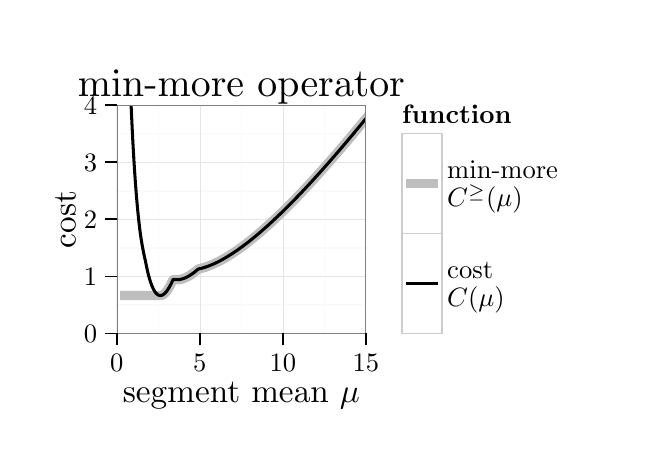
\begin{tikzpicture}[x=1pt,y=1pt]
\definecolor{fillColor}{RGB}{255,255,255}
\path[use as bounding box,fill=fillColor,fill opacity=0.00] (0,0) rectangle (216.81,144.54);
\begin{scope}
\path[clip] (  0.00,  0.00) rectangle (216.81,144.54);
\definecolor{drawColor}{RGB}{255,255,255}
\definecolor{fillColor}{RGB}{255,255,255}

\path[draw=drawColor,line width= 0.6pt,line join=round,line cap=round,fill=fillColor] (  0.00, -0.00) rectangle (216.81,144.54);
\end{scope}
\begin{scope}
\path[clip] ( 32.22, 34.03) rectangle (122.22,116.55);
\definecolor{fillColor}{RGB}{255,255,255}

\path[fill=fillColor] ( 32.22, 34.03) rectangle (122.22,116.55);
\definecolor{drawColor}{gray}{0.98}

\path[draw=drawColor,line width= 0.6pt,line join=round] ( 32.22, 44.35) --
	(122.22, 44.35);

\path[draw=drawColor,line width= 0.6pt,line join=round] ( 32.22, 64.98) --
	(122.22, 64.98);

\path[draw=drawColor,line width= 0.6pt,line join=round] ( 32.22, 85.61) --
	(122.22, 85.61);

\path[draw=drawColor,line width= 0.6pt,line join=round] ( 32.22,106.24) --
	(122.22,106.24);

\path[draw=drawColor,line width= 0.6pt,line join=round] ( 47.22, 34.03) --
	( 47.22,116.55);

\path[draw=drawColor,line width= 0.6pt,line join=round] ( 77.22, 34.03) --
	( 77.22,116.55);

\path[draw=drawColor,line width= 0.6pt,line join=round] (107.22, 34.03) --
	(107.22,116.55);
\definecolor{drawColor}{gray}{0.90}

\path[draw=drawColor,line width= 0.2pt,line join=round] ( 32.22, 34.03) --
	(122.22, 34.03);

\path[draw=drawColor,line width= 0.2pt,line join=round] ( 32.22, 54.66) --
	(122.22, 54.66);

\path[draw=drawColor,line width= 0.2pt,line join=round] ( 32.22, 75.29) --
	(122.22, 75.29);

\path[draw=drawColor,line width= 0.2pt,line join=round] ( 32.22, 95.92) --
	(122.22, 95.92);

\path[draw=drawColor,line width= 0.2pt,line join=round] ( 32.22,116.55) --
	(122.22,116.55);

\path[draw=drawColor,line width= 0.2pt,line join=round] ( 32.22, 34.03) --
	( 32.22,116.55);

\path[draw=drawColor,line width= 0.2pt,line join=round] ( 62.22, 34.03) --
	( 62.22,116.55);

\path[draw=drawColor,line width= 0.2pt,line join=round] ( 92.22, 34.03) --
	( 92.22,116.55);

\path[draw=drawColor,line width= 0.2pt,line join=round] (122.22, 34.03) --
	(122.22,116.55);
\definecolor{drawColor}{RGB}{190,190,190}

\path[draw=drawColor,line width= 3.4pt,line join=round] ( 33.40, 47.76) --
	( 33.55, 47.76) --
	( 33.70, 47.76) --
	( 33.84, 47.76) --
	( 33.99, 47.76) --
	( 34.14, 47.76) --
	( 34.28, 47.76) --
	( 34.43, 47.76) --
	( 34.58, 47.76) --
	( 34.73, 47.76) --
	( 34.87, 47.76) --
	( 35.02, 47.76) --
	( 35.17, 47.76) --
	( 35.31, 47.76) --
	( 35.46, 47.76) --
	( 35.61, 47.76) --
	( 35.75, 47.76) --
	( 35.90, 47.76) --
	( 36.05, 47.76) --
	( 36.19, 47.76) --
	( 36.34, 47.76) --
	( 36.49, 47.76) --
	( 36.63, 47.76) --
	( 36.78, 47.76) --
	( 36.93, 47.76) --
	( 37.08, 47.76) --
	( 37.22, 47.76) --
	( 37.37, 47.76) --
	( 37.52, 47.76) --
	( 37.66, 47.76) --
	( 37.81, 47.76) --
	( 37.96, 47.76) --
	( 38.10, 47.76) --
	( 38.25, 47.76) --
	( 38.40, 47.76) --
	( 38.54, 47.76) --
	( 38.69, 47.76) --
	( 38.84, 47.76) --
	( 38.98, 47.76) --
	( 39.13, 47.76) --
	( 39.28, 47.76) --
	( 39.43, 47.76) --
	( 39.57, 47.76) --
	( 39.72, 47.76) --
	( 39.87, 47.76) --
	( 40.01, 47.76) --
	( 40.16, 47.76) --
	( 40.31, 47.76) --
	( 40.45, 47.76) --
	( 40.60, 47.76) --
	( 40.75, 47.76) --
	( 40.89, 47.76) --
	( 41.04, 47.76) --
	( 41.19, 47.76) --
	( 41.34, 47.76) --
	( 41.48, 47.76) --
	( 41.63, 47.76) --
	( 41.78, 47.76) --
	( 41.92, 47.76) --
	( 42.07, 47.76) --
	( 42.22, 47.76) --
	( 42.36, 47.76) --
	( 42.51, 47.76) --
	( 42.66, 47.76) --
	( 42.80, 47.76) --
	( 42.95, 47.76) --
	( 43.10, 47.76) --
	( 43.24, 47.76) --
	( 43.39, 47.76) --
	( 43.54, 47.76) --
	( 43.69, 47.76) --
	( 43.83, 47.76) --
	( 43.98, 47.76) --
	( 44.13, 47.76) --
	( 44.27, 47.76) --
	( 44.42, 47.76) --
	( 44.57, 47.76) --
	( 44.71, 47.76) --
	( 44.86, 47.76) --
	( 45.01, 47.76) --
	( 45.15, 47.76) --
	( 45.30, 47.76) --
	( 45.45, 47.76) --
	( 45.59, 47.76) --
	( 45.74, 47.76) --
	( 45.89, 47.76) --
	( 46.04, 47.76) --
	( 46.18, 47.76) --
	( 46.33, 47.76) --
	( 46.48, 47.76) --
	( 46.62, 47.76) --
	( 46.77, 47.76) --
	( 46.92, 47.76) --
	( 47.06, 47.76) --
	( 47.21, 47.76) --
	( 47.36, 47.76) --
	( 47.50, 47.76) --
	( 47.65, 47.76) --
	( 47.80, 47.76) --
	( 47.94, 47.76) --
	( 47.94, 47.76) --
	( 47.99, 47.76) --
	( 48.04, 47.76) --
	( 48.08, 47.76) --
	( 48.13, 47.77) --
	( 48.17, 47.77) --
	( 48.22, 47.78) --
	( 48.27, 47.79) --
	( 48.31, 47.80) --
	( 48.36, 47.81) --
	( 48.40, 47.82) --
	( 48.45, 47.84) --
	( 48.50, 47.85) --
	( 48.54, 47.87) --
	( 48.59, 47.89) --
	( 48.63, 47.91) --
	( 48.68, 47.93) --
	( 48.73, 47.95) --
	( 48.77, 47.97) --
	( 48.82, 48.00) --
	( 48.86, 48.02) --
	( 48.91, 48.05) --
	( 48.95, 48.08) --
	( 49.00, 48.11) --
	( 49.05, 48.14) --
	( 49.09, 48.17) --
	( 49.14, 48.20) --
	( 49.18, 48.24) --
	( 49.23, 48.27) --
	( 49.28, 48.31) --
	( 49.32, 48.35) --
	( 49.37, 48.38) --
	( 49.41, 48.42) --
	( 49.46, 48.47) --
	( 49.51, 48.51) --
	( 49.55, 48.55) --
	( 49.60, 48.60) --
	( 49.64, 48.64) --
	( 49.69, 48.69) --
	( 49.74, 48.74) --
	( 49.78, 48.78) --
	( 49.83, 48.83) --
	( 49.87, 48.89) --
	( 49.92, 48.94) --
	( 49.97, 48.99) --
	( 50.01, 49.05) --
	( 50.06, 49.10) --
	( 50.10, 49.16) --
	( 50.15, 49.22) --
	( 50.19, 49.27) --
	( 50.24, 49.33) --
	( 50.29, 49.40) --
	( 50.33, 49.46) --
	( 50.38, 49.52) --
	( 50.42, 49.58) --
	( 50.47, 49.65) --
	( 50.52, 49.72) --
	( 50.56, 49.78) --
	( 50.61, 49.85) --
	( 50.65, 49.92) --
	( 50.70, 49.99) --
	( 50.75, 50.06) --
	( 50.79, 50.13) --
	( 50.84, 50.21) --
	( 50.88, 50.28) --
	( 50.93, 50.36) --
	( 50.98, 50.43) --
	( 51.02, 50.51) --
	( 51.07, 50.59) --
	( 51.11, 50.67) --
	( 51.16, 50.75) --
	( 51.21, 50.83) --
	( 51.25, 50.91) --
	( 51.30, 50.99) --
	( 51.34, 51.07) --
	( 51.39, 51.16) --
	( 51.43, 51.25) --
	( 51.48, 51.33) --
	( 51.53, 51.42) --
	( 51.57, 51.51) --
	( 51.62, 51.60) --
	( 51.66, 51.69) --
	( 51.71, 51.78) --
	( 51.76, 51.87) --
	( 51.80, 51.96) --
	( 51.85, 52.06) --
	( 51.89, 52.15) --
	( 51.94, 52.25) --
	( 51.99, 52.34) --
	( 52.03, 52.44) --
	( 52.08, 52.54) --
	( 52.12, 52.64) --
	( 52.17, 52.74) --
	( 52.22, 52.84) --
	( 52.26, 52.94) --
	( 52.31, 53.04) --
	( 52.35, 53.15) --
	( 52.40, 53.25) --
	( 52.45, 53.35) --
	( 52.49, 53.46) --
	( 52.49, 53.46) --
	( 52.50, 53.46) --
	( 52.52, 53.46) --
	( 52.53, 53.46) --
	( 52.55, 53.46) --
	( 52.56, 53.46) --
	( 52.57, 53.46) --
	( 52.59, 53.46) --
	( 52.60, 53.46) --
	( 52.62, 53.46) --
	( 52.63, 53.46) --
	( 52.64, 53.46) --
	( 52.66, 53.46) --
	( 52.67, 53.46) --
	( 52.68, 53.46) --
	( 52.70, 53.46) --
	( 52.71, 53.46) --
	( 52.73, 53.46) --
	( 52.74, 53.46) --
	( 52.75, 53.46) --
	( 52.77, 53.46) --
	( 52.78, 53.46) --
	( 52.80, 53.46) --
	( 52.81, 53.46) --
	( 52.82, 53.46) --
	( 52.84, 53.46) --
	( 52.85, 53.46) --
	( 52.86, 53.46) --
	( 52.88, 53.46) --
	( 52.89, 53.46) --
	( 52.91, 53.46) --
	( 52.92, 53.46) --
	( 52.93, 53.46) --
	( 52.95, 53.46) --
	( 52.96, 53.46) --
	( 52.97, 53.46) --
	( 52.99, 53.46) --
	( 53.00, 53.46) --
	( 53.02, 53.46) --
	( 53.03, 53.46) --
	( 53.04, 53.46) --
	( 53.06, 53.46) --
	( 53.07, 53.46) --
	( 53.09, 53.46) --
	( 53.10, 53.46) --
	( 53.11, 53.46) --
	( 53.13, 53.46) --
	( 53.14, 53.46) --
	( 53.15, 53.46) --
	( 53.17, 53.46) --
	( 53.18, 53.46) --
	( 53.20, 53.46) --
	( 53.21, 53.46) --
	( 53.22, 53.46) --
	( 53.24, 53.46) --
	( 53.25, 53.46) --
	( 53.26, 53.46) --
	( 53.28, 53.46) --
	( 53.29, 53.46) --
	( 53.31, 53.46) --
	( 53.32, 53.46) --
	( 53.33, 53.46) --
	( 53.35, 53.46) --
	( 53.36, 53.46) --
	( 53.38, 53.46) --
	( 53.39, 53.46) --
	( 53.40, 53.46) --
	( 53.42, 53.46) --
	( 53.43, 53.46) --
	( 53.44, 53.46) --
	( 53.46, 53.46) --
	( 53.47, 53.46) --
	( 53.49, 53.46) --
	( 53.50, 53.46) --
	( 53.51, 53.46) --
	( 53.53, 53.46) --
	( 53.54, 53.46) --
	( 53.56, 53.46) --
	( 53.57, 53.46) --
	( 53.58, 53.46) --
	( 53.60, 53.46) --
	( 53.61, 53.46) --
	( 53.62, 53.46) --
	( 53.64, 53.46) --
	( 53.65, 53.46) --
	( 53.67, 53.46) --
	( 53.68, 53.46) --
	( 53.69, 53.46) --
	( 53.71, 53.46) --
	( 53.72, 53.46) --
	( 53.73, 53.46) --
	( 53.75, 53.46) --
	( 53.76, 53.46) --
	( 53.78, 53.46) --
	( 53.79, 53.46) --
	( 53.80, 53.46) --
	( 53.82, 53.46) --
	( 53.83, 53.46) --
	( 53.85, 53.46) --
	( 53.86, 53.46) --
	( 53.86, 53.46) --
	( 53.94, 53.46) --
	( 54.02, 53.46) --
	( 54.09, 53.47) --
	( 54.17, 53.47) --
	( 54.25, 53.47) --
	( 54.33, 53.48) --
	( 54.41, 53.48) --
	( 54.48, 53.49) --
	( 54.56, 53.50) --
	( 54.64, 53.51) --
	( 54.72, 53.52) --
	( 54.80, 53.53) --
	( 54.87, 53.54) --
	( 54.95, 53.55) --
	( 55.03, 53.57) --
	( 55.11, 53.58) --
	( 55.19, 53.60) --
	( 55.26, 53.61) --
	( 55.34, 53.63) --
	( 55.42, 53.65) --
	( 55.50, 53.66) --
	( 55.58, 53.68) --
	( 55.65, 53.70) --
	( 55.73, 53.72) --
	( 55.81, 53.75) --
	( 55.89, 53.77) --
	( 55.97, 53.79) --
	( 56.04, 53.82) --
	( 56.12, 53.84) --
	( 56.20, 53.87) --
	( 56.28, 53.89) --
	( 56.36, 53.92) --
	( 56.43, 53.95) --
	( 56.51, 53.98) --
	( 56.59, 54.01) --
	( 56.67, 54.04) --
	( 56.75, 54.07) --
	( 56.82, 54.10) --
	( 56.90, 54.13) --
	( 56.98, 54.17) --
	( 57.06, 54.20) --
	( 57.14, 54.24) --
	( 57.21, 54.27) --
	( 57.29, 54.31) --
	( 57.37, 54.35) --
	( 57.45, 54.38) --
	( 57.53, 54.42) --
	( 57.60, 54.46) --
	( 57.68, 54.50) --
	( 57.76, 54.54) --
	( 57.84, 54.58) --
	( 57.92, 54.62) --
	( 57.99, 54.67) --
	( 58.07, 54.71) --
	( 58.15, 54.75) --
	( 58.23, 54.80) --
	( 58.31, 54.84) --
	( 58.38, 54.89) --
	( 58.46, 54.94) --
	( 58.54, 54.98) --
	( 58.62, 55.03) --
	( 58.70, 55.08) --
	( 58.77, 55.13) --
	( 58.85, 55.18) --
	( 58.93, 55.23) --
	( 59.01, 55.28) --
	( 59.09, 55.33) --
	( 59.16, 55.39) --
	( 59.24, 55.44) --
	( 59.32, 55.49) --
	( 59.40, 55.55) --
	( 59.48, 55.60) --
	( 59.55, 55.66) --
	( 59.63, 55.72) --
	( 59.71, 55.77) --
	( 59.79, 55.83) --
	( 59.87, 55.89) --
	( 59.94, 55.95) --
	( 60.02, 56.00) --
	( 60.10, 56.06) --
	( 60.18, 56.13) --
	( 60.26, 56.19) --
	( 60.33, 56.25) --
	( 60.41, 56.31) --
	( 60.49, 56.37) --
	( 60.57, 56.44) --
	( 60.65, 56.50) --
	( 60.72, 56.56) --
	( 60.80, 56.63) --
	( 60.88, 56.69) --
	( 60.96, 56.76) --
	( 61.04, 56.83) --
	( 61.11, 56.89) --
	( 61.19, 56.96) --
	( 61.27, 57.03) --
	( 61.35, 57.10) --
	( 61.43, 57.17) --
	( 61.50, 57.24) --
	( 61.58, 57.31) --
	( 61.58, 57.31) --
	( 62.58, 57.54) --
	( 63.58, 57.81) --
	( 64.59, 58.14) --
	( 65.59, 58.50) --
	( 66.59, 58.91) --
	( 67.59, 59.35) --
	( 68.59, 59.83) --
	( 69.60, 60.34) --
	( 70.60, 60.89) --
	( 71.60, 61.46) --
	( 72.60, 62.07) --
	( 73.60, 62.70) --
	( 74.60, 63.36) --
	( 75.61, 64.04) --
	( 76.61, 64.75) --
	( 77.61, 65.47) --
	( 78.61, 66.23) --
	( 79.61, 67.00) --
	( 80.62, 67.79) --
	( 81.62, 68.60) --
	( 82.62, 69.43) --
	( 83.62, 70.27) --
	( 84.62, 71.14) --
	( 85.62, 72.02) --
	( 86.63, 72.91) --
	( 87.63, 73.82) --
	( 88.63, 74.75) --
	( 89.63, 75.69) --
	( 90.63, 76.64) --
	( 91.63, 77.60) --
	( 92.64, 78.58) --
	( 93.64, 79.57) --
	( 94.64, 80.57) --
	( 95.64, 81.59) --
	( 96.64, 82.61) --
	( 97.65, 83.65) --
	( 98.65, 84.69) --
	( 99.65, 85.75) --
	(100.65, 86.82) --
	(101.65, 87.89) --
	(102.65, 88.98) --
	(103.66, 90.07) --
	(104.66, 91.17) --
	(105.66, 92.28) --
	(106.66, 93.40) --
	(107.66, 94.53) --
	(108.66, 95.66) --
	(109.67, 96.81) --
	(110.67, 97.96) --
	(111.67, 99.12) --
	(112.67,100.28) --
	(113.67,101.45) --
	(114.68,102.63) --
	(115.68,103.81) --
	(116.68,105.01) --
	(117.68,106.20) --
	(118.68,107.41) --
	(119.68,108.62) --
	(120.69,109.83) --
	(121.69,111.05) --
	(122.69,112.28) --
	(123.69,113.51) --
	(124.69,114.75) --
	(125.69,115.99) --
	(126.70,117.24) --
	(127.70,118.49) --
	(128.70,119.75) --
	(129.70,121.01) --
	(130.70,122.28) --
	(131.71,123.55) --
	(132.71,124.83) --
	(133.71,126.11) --
	(134.71,127.39) --
	(135.71,128.68) --
	(136.71,129.98) --
	(137.72,131.28) --
	(138.72,132.58) --
	(139.72,133.88) --
	(140.72,135.19) --
	(141.72,136.51) --
	(142.73,137.82) --
	(143.73,139.14) --
	(144.73,140.47) --
	(145.73,141.80) --
	(146.73,143.13) --
	(147.73,144.46) --
	(147.79,144.54);
\definecolor{drawColor}{RGB}{0,0,0}

\path[draw=drawColor,line width= 1.1pt,line join=round] ( 36.37,144.54) --
	( 36.37,144.21) --
	( 36.45,141.63) --
	( 36.53,139.12) --
	( 36.61,136.68) --
	( 36.69,134.31) --
	( 36.77,132.01) --
	( 36.85,129.77) --
	( 36.93,127.59) --
	( 37.01,125.48) --
	( 37.09,123.42) --
	( 37.17,121.41) --
	( 37.25,119.46) --
	( 37.33,117.56) --
	( 37.41,115.72) --
	( 37.49,113.92) --
	( 37.57,112.17) --
	( 37.65,110.46) --
	( 37.73,108.80) --
	( 37.81,107.19) --
	( 37.89,105.61) --
	( 37.97,104.08) --
	( 38.05,102.59) --
	( 38.13,101.14) --
	( 38.21, 99.72) --
	( 38.29, 98.34) --
	( 38.37, 97.00) --
	( 38.45, 95.69) --
	( 38.53, 94.42) --
	( 38.61, 93.18) --
	( 38.69, 91.97) --
	( 38.77, 90.79) --
	( 38.85, 89.65) --
	( 38.93, 88.53) --
	( 39.01, 87.45) --
	( 39.09, 86.39) --
	( 39.17, 85.36) --
	( 39.25, 84.36) --
	( 39.33, 83.39) --
	( 39.41, 82.44) --
	( 39.49, 81.52) --
	( 39.57, 80.62) --
	( 39.65, 79.74) --
	( 39.73, 78.90) --
	( 39.81, 78.07) --
	( 39.89, 77.27) --
	( 39.97, 76.49) --
	( 40.05, 75.73) --
	( 40.13, 74.99) --
	( 40.21, 74.28) --
	( 40.29, 73.58) --
	( 40.37, 72.91) --
	( 40.44, 72.25) --
	( 40.52, 71.62) --
	( 40.60, 71.00) --
	( 40.68, 70.41) --
	( 40.76, 69.83) --
	( 40.84, 69.27) --
	( 40.92, 68.73) --
	( 41.00, 68.20) --
	( 41.08, 67.69) --
	( 41.16, 67.20) --
	( 41.24, 66.73) --
	( 41.32, 66.27) --
	( 41.40, 65.83) --
	( 41.48, 65.40) --
	( 41.56, 64.99) --
	( 41.56, 64.99) --
	( 41.57, 64.93) --
	( 41.58, 64.88) --
	( 41.59, 64.82) --
	( 41.60, 64.76) --
	( 41.61, 64.71) --
	( 41.62, 64.65) --
	( 41.63, 64.59) --
	( 41.64, 64.54) --
	( 41.65, 64.48) --
	( 41.66, 64.43) --
	( 41.67, 64.37) --
	( 41.68, 64.32) --
	( 41.69, 64.26) --
	( 41.70, 64.21) --
	( 41.71, 64.15) --
	( 41.72, 64.10) --
	( 41.73, 64.04) --
	( 41.74, 63.99) --
	( 41.75, 63.94) --
	( 41.76, 63.88) --
	( 41.77, 63.83) --
	( 41.78, 63.78) --
	( 41.79, 63.72) --
	( 41.80, 63.67) --
	( 41.81, 63.62) --
	( 41.82, 63.57) --
	( 41.83, 63.52) --
	( 41.84, 63.46) --
	( 41.85, 63.41) --
	( 41.86, 63.36) --
	( 41.87, 63.31) --
	( 41.88, 63.26) --
	( 41.89, 63.21) --
	( 41.90, 63.16) --
	( 41.91, 63.11) --
	( 41.92, 63.06) --
	( 41.93, 63.01) --
	( 41.94, 62.96) --
	( 41.95, 62.91) --
	( 41.96, 62.86) --
	( 41.97, 62.81) --
	( 41.98, 62.76) --
	( 41.99, 62.71) --
	( 42.00, 62.67) --
	( 42.01, 62.62) --
	( 42.02, 62.57) --
	( 42.03, 62.52) --
	( 42.04, 62.48) --
	( 42.05, 62.43) --
	( 42.06, 62.38) --
	( 42.07, 62.33) --
	( 42.08, 62.29) --
	( 42.09, 62.24) --
	( 42.10, 62.19) --
	( 42.11, 62.15) --
	( 42.12, 62.10) --
	( 42.13, 62.06) --
	( 42.14, 62.01) --
	( 42.15, 61.97) --
	( 42.16, 61.92) --
	( 42.17, 61.88) --
	( 42.18, 61.83) --
	( 42.19, 61.79) --
	( 42.20, 61.74) --
	( 42.21, 61.70) --
	( 42.22, 61.65) --
	( 42.22, 61.61) --
	( 42.23, 61.57) --
	( 42.24, 61.52) --
	( 42.25, 61.48) --
	( 42.26, 61.44) --
	( 42.27, 61.39) --
	( 42.28, 61.35) --
	( 42.29, 61.31) --
	( 42.30, 61.27) --
	( 42.31, 61.23) --
	( 42.32, 61.18) --
	( 42.33, 61.14) --
	( 42.34, 61.10) --
	( 42.35, 61.06) --
	( 42.36, 61.02) --
	( 42.37, 60.98) --
	( 42.38, 60.94) --
	( 42.39, 60.90) --
	( 42.40, 60.86) --
	( 42.41, 60.82) --
	( 42.42, 60.78) --
	( 42.43, 60.74) --
	( 42.44, 60.70) --
	( 42.45, 60.66) --
	( 42.46, 60.62) --
	( 42.47, 60.58) --
	( 42.48, 60.54) --
	( 42.49, 60.50) --
	( 42.50, 60.46) --
	( 42.51, 60.43) --
	( 42.52, 60.39) --
	( 42.53, 60.35) --
	( 42.54, 60.31) --
	( 42.54, 60.31) --
	( 42.64, 59.77) --
	( 42.74, 59.25) --
	( 42.84, 58.74) --
	( 42.95, 58.25) --
	( 43.05, 57.77) --
	( 43.15, 57.31) --
	( 43.25, 56.85) --
	( 43.35, 56.42) --
	( 43.45, 55.99) --
	( 43.55, 55.58) --
	( 43.65, 55.18) --
	( 43.75, 54.80) --
	( 43.86, 54.43) --
	( 43.96, 54.07) --
	( 44.06, 53.72) --
	( 44.16, 53.38) --
	( 44.26, 53.06) --
	( 44.36, 52.74) --
	( 44.46, 52.44) --
	( 44.56, 52.15) --
	( 44.66, 51.87) --
	( 44.77, 51.60) --
	( 44.87, 51.34) --
	( 44.97, 51.09) --
	( 45.07, 50.85) --
	( 45.17, 50.62) --
	( 45.27, 50.41) --
	( 45.37, 50.20) --
	( 45.47, 50.00) --
	( 45.57, 49.81) --
	( 45.68, 49.63) --
	( 45.78, 49.46) --
	( 45.88, 49.29) --
	( 45.98, 49.14) --
	( 46.08, 49.00) --
	( 46.18, 48.86) --
	( 46.28, 48.73) --
	( 46.38, 48.61) --
	( 46.48, 48.50) --
	( 46.59, 48.40) --
	( 46.69, 48.30) --
	( 46.79, 48.22) --
	( 46.89, 48.14) --
	( 46.99, 48.07) --
	( 47.09, 48.00) --
	( 47.19, 47.95) --
	( 47.29, 47.90) --
	( 47.40, 47.86) --
	( 47.50, 47.82) --
	( 47.60, 47.80) --
	( 47.70, 47.78) --
	( 47.80, 47.76) --
	( 47.90, 47.76) --
	( 48.00, 47.76) --
	( 48.10, 47.77) --
	( 48.20, 47.78) --
	( 48.31, 47.80) --
	( 48.41, 47.83) --
	( 48.51, 47.86) --
	( 48.61, 47.90) --
	( 48.71, 47.94) --
	( 48.81, 47.99) --
	( 48.91, 48.05) --
	( 49.01, 48.12) --
	( 49.11, 48.18) --
	( 49.22, 48.26) --
	( 49.32, 48.34) --
	( 49.42, 48.43) --
	( 49.52, 48.52) --
	( 49.62, 48.62) --
	( 49.72, 48.72) --
	( 49.82, 48.83) --
	( 49.92, 48.94) --
	( 50.02, 49.06) --
	( 50.13, 49.19) --
	( 50.23, 49.32) --
	( 50.33, 49.45) --
	( 50.43, 49.59) --
	( 50.53, 49.73) --
	( 50.63, 49.88) --
	( 50.73, 50.04) --
	( 50.83, 50.20) --
	( 50.93, 50.36) --
	( 51.04, 50.53) --
	( 51.14, 50.71) --
	( 51.24, 50.88) --
	( 51.34, 51.07) --
	( 51.44, 51.25) --
	( 51.54, 51.45) --
	( 51.64, 51.64) --
	( 51.74, 51.84) --
	( 51.84, 52.05) --
	( 51.95, 52.26) --
	( 52.05, 52.47) --
	( 52.15, 52.69) --
	( 52.25, 52.91) --
	( 52.35, 53.14) --
	( 52.45, 53.37) --
	( 52.55, 53.60) --
	( 52.55, 53.60) --
	( 52.64, 53.58) --
	( 52.73, 53.57) --
	( 52.83, 53.55) --
	( 52.92, 53.53) --
	( 53.01, 53.52) --
	( 53.10, 53.51) --
	( 53.19, 53.50) --
	( 53.28, 53.49) --
	( 53.37, 53.48) --
	( 53.46, 53.47) --
	( 53.56, 53.47) --
	( 53.65, 53.46) --
	( 53.74, 53.46) --
	( 53.83, 53.46) --
	( 53.92, 53.46) --
	( 54.01, 53.46) --
	( 54.10, 53.47) --
	( 54.19, 53.47) --
	( 54.28, 53.48) --
	( 54.38, 53.48) --
	( 54.47, 53.49) --
	( 54.56, 53.50) --
	( 54.65, 53.51) --
	( 54.74, 53.52) --
	( 54.83, 53.53) --
	( 54.92, 53.55) --
	( 55.01, 53.56) --
	( 55.11, 53.58) --
	( 55.20, 53.60) --
	( 55.29, 53.62) --
	( 55.38, 53.64) --
	( 55.47, 53.66) --
	( 55.56, 53.68) --
	( 55.65, 53.70) --
	( 55.74, 53.73) --
	( 55.84, 53.75) --
	( 55.93, 53.78) --
	( 56.02, 53.81) --
	( 56.11, 53.84) --
	( 56.20, 53.87) --
	( 56.29, 53.90) --
	( 56.38, 53.93) --
	( 56.47, 53.96) --
	( 56.56, 54.00) --
	( 56.66, 54.03) --
	( 56.75, 54.07) --
	( 56.84, 54.11) --
	( 56.93, 54.15) --
	( 57.02, 54.19) --
	( 57.11, 54.23) --
	( 57.20, 54.27) --
	( 57.29, 54.31) --
	( 57.39, 54.35) --
	( 57.48, 54.40) --
	( 57.57, 54.44) --
	( 57.66, 54.49) --
	( 57.75, 54.54) --
	( 57.84, 54.59) --
	( 57.93, 54.63) --
	( 58.02, 54.68) --
	( 58.12, 54.74) --
	( 58.21, 54.79) --
	( 58.30, 54.84) --
	( 58.39, 54.89) --
	( 58.48, 54.95) --
	( 58.57, 55.00) --
	( 58.66, 55.06) --
	( 58.75, 55.12) --
	( 58.85, 55.18) --
	( 58.94, 55.24) --
	( 59.03, 55.30) --
	( 59.12, 55.36) --
	( 59.21, 55.42) --
	( 59.30, 55.48) --
	( 59.39, 55.54) --
	( 59.48, 55.61) --
	( 59.57, 55.67) --
	( 59.67, 55.74) --
	( 59.76, 55.81) --
	( 59.85, 55.87) --
	( 59.94, 55.94) --
	( 60.03, 56.01) --
	( 60.12, 56.08) --
	( 60.21, 56.15) --
	( 60.30, 56.22) --
	( 60.40, 56.30) --
	( 60.49, 56.37) --
	( 60.58, 56.44) --
	( 60.67, 56.52) --
	( 60.76, 56.59) --
	( 60.85, 56.67) --
	( 60.94, 56.75) --
	( 61.03, 56.83) --
	( 61.13, 56.90) --
	( 61.22, 56.98) --
	( 61.31, 57.06) --
	( 61.40, 57.14) --
	( 61.49, 57.22) --
	( 61.58, 57.31) --
	( 61.58, 57.31) --
	( 62.58, 57.54) --
	( 63.58, 57.81) --
	( 64.59, 58.14) --
	( 65.59, 58.50) --
	( 66.59, 58.91) --
	( 67.59, 59.35) --
	( 68.59, 59.83) --
	( 69.60, 60.34) --
	( 70.60, 60.89) --
	( 71.60, 61.46) --
	( 72.60, 62.07) --
	( 73.60, 62.70) --
	( 74.60, 63.36) --
	( 75.61, 64.04) --
	( 76.61, 64.75) --
	( 77.61, 65.47) --
	( 78.61, 66.23) --
	( 79.61, 67.00) --
	( 80.62, 67.79) --
	( 81.62, 68.60) --
	( 82.62, 69.43) --
	( 83.62, 70.27) --
	( 84.62, 71.14) --
	( 85.62, 72.02) --
	( 86.63, 72.91) --
	( 87.63, 73.82) --
	( 88.63, 74.75) --
	( 89.63, 75.69) --
	( 90.63, 76.64) --
	( 91.63, 77.60) --
	( 92.64, 78.58) --
	( 93.64, 79.57) --
	( 94.64, 80.57) --
	( 95.64, 81.59) --
	( 96.64, 82.61) --
	( 97.65, 83.65) --
	( 98.65, 84.69) --
	( 99.65, 85.75) --
	(100.65, 86.82) --
	(101.65, 87.89) --
	(102.65, 88.98) --
	(103.66, 90.07) --
	(104.66, 91.17) --
	(105.66, 92.28) --
	(106.66, 93.40) --
	(107.66, 94.53) --
	(108.66, 95.66) --
	(109.67, 96.81) --
	(110.67, 97.96) --
	(111.67, 99.12) --
	(112.67,100.28) --
	(113.67,101.45) --
	(114.68,102.63) --
	(115.68,103.81) --
	(116.68,105.01) --
	(117.68,106.20) --
	(118.68,107.41) --
	(119.68,108.62) --
	(120.69,109.83) --
	(121.69,111.05) --
	(122.69,112.28) --
	(123.69,113.51) --
	(124.69,114.75) --
	(125.69,115.99) --
	(126.70,117.24) --
	(127.70,118.49) --
	(128.70,119.75) --
	(129.70,121.01) --
	(130.70,122.28) --
	(131.71,123.55) --
	(132.71,124.83) --
	(133.71,126.11) --
	(134.71,127.39) --
	(135.71,128.68) --
	(136.71,129.98) --
	(137.72,131.28) --
	(138.72,132.58) --
	(139.72,133.88) --
	(140.72,135.19) --
	(141.72,136.51) --
	(142.73,137.82) --
	(143.73,139.14) --
	(144.73,140.47) --
	(145.73,141.80) --
	(146.73,143.13) --
	(147.73,144.46) --
	(147.79,144.54);
\definecolor{drawColor}{gray}{0.50}

\path[draw=drawColor,line width= 0.6pt,line join=round,line cap=round] ( 32.22, 34.03) rectangle (122.22,116.55);
\end{scope}
\begin{scope}
\path[clip] (  0.00,  0.00) rectangle (216.81,144.54);
\definecolor{drawColor}{RGB}{0,0,0}

\node[text=drawColor,anchor=base east,inner sep=0pt, outer sep=0pt, scale=  0.96] at ( 25.11, 30.73) {0};

\node[text=drawColor,anchor=base east,inner sep=0pt, outer sep=0pt, scale=  0.96] at ( 25.11, 51.36) {1};

\node[text=drawColor,anchor=base east,inner sep=0pt, outer sep=0pt, scale=  0.96] at ( 25.11, 71.99) {2};

\node[text=drawColor,anchor=base east,inner sep=0pt, outer sep=0pt, scale=  0.96] at ( 25.11, 92.62) {3};

\node[text=drawColor,anchor=base east,inner sep=0pt, outer sep=0pt, scale=  0.96] at ( 25.11,113.25) {4};
\end{scope}
\begin{scope}
\path[clip] (  0.00,  0.00) rectangle (216.81,144.54);
\definecolor{drawColor}{RGB}{0,0,0}

\path[draw=drawColor,line width= 0.6pt,line join=round] ( 27.95, 34.03) --
	( 32.22, 34.03);

\path[draw=drawColor,line width= 0.6pt,line join=round] ( 27.95, 54.66) --
	( 32.22, 54.66);

\path[draw=drawColor,line width= 0.6pt,line join=round] ( 27.95, 75.29) --
	( 32.22, 75.29);

\path[draw=drawColor,line width= 0.6pt,line join=round] ( 27.95, 95.92) --
	( 32.22, 95.92);

\path[draw=drawColor,line width= 0.6pt,line join=round] ( 27.95,116.55) --
	( 32.22,116.55);
\end{scope}
\begin{scope}
\path[clip] (  0.00,  0.00) rectangle (216.81,144.54);
\definecolor{drawColor}{RGB}{0,0,0}

\path[draw=drawColor,line width= 0.6pt,line join=round] ( 32.22, 29.77) --
	( 32.22, 34.03);

\path[draw=drawColor,line width= 0.6pt,line join=round] ( 62.22, 29.77) --
	( 62.22, 34.03);

\path[draw=drawColor,line width= 0.6pt,line join=round] ( 92.22, 29.77) --
	( 92.22, 34.03);

\path[draw=drawColor,line width= 0.6pt,line join=round] (122.22, 29.77) --
	(122.22, 34.03);
\end{scope}
\begin{scope}
\path[clip] (  0.00,  0.00) rectangle (216.81,144.54);
\definecolor{drawColor}{RGB}{0,0,0}

\node[text=drawColor,anchor=base,inner sep=0pt, outer sep=0pt, scale=  0.96] at ( 32.22, 20.31) {0};

\node[text=drawColor,anchor=base,inner sep=0pt, outer sep=0pt, scale=  0.96] at ( 62.22, 20.31) {5};

\node[text=drawColor,anchor=base,inner sep=0pt, outer sep=0pt, scale=  0.96] at ( 92.22, 20.31) {10};

\node[text=drawColor,anchor=base,inner sep=0pt, outer sep=0pt, scale=  0.96] at (122.22, 20.31) {15};
\end{scope}
\begin{scope}
\path[clip] (  0.00,  0.00) rectangle (216.81,144.54);
\definecolor{drawColor}{RGB}{0,0,0}

\node[text=drawColor,anchor=base,inner sep=0pt, outer sep=0pt, scale=  1.20] at ( 77.22,  9.03) {segment mean $\mu$};
\end{scope}
\begin{scope}
\path[clip] (  0.00,  0.00) rectangle (216.81,144.54);
\definecolor{drawColor}{RGB}{0,0,0}

\node[text=drawColor,rotate= 90.00,anchor=base,inner sep=0pt, outer sep=0pt, scale=  1.20] at ( 17.30, 75.29) {cost};
\end{scope}
\begin{scope}
\path[clip] (  0.00,  0.00) rectangle (216.81,144.54);
\definecolor{fillColor}{RGB}{255,255,255}

\path[fill=fillColor] (131.08, 29.77) rectangle (195.90,120.82);
\end{scope}
\begin{scope}
\path[clip] (  0.00,  0.00) rectangle (216.81,144.54);
\definecolor{drawColor}{RGB}{0,0,0}

\node[text=drawColor,anchor=base west,inner sep=0pt, outer sep=0pt, scale=  0.96] at (135.35,109.92) {\bfseries function};
\end{scope}
\begin{scope}
\path[clip] (  0.00,  0.00) rectangle (216.81,144.54);
\definecolor{drawColor}{gray}{0.80}
\definecolor{fillColor}{RGB}{255,255,255}

\path[draw=drawColor,line width= 0.6pt,line join=round,line cap=round,fill=fillColor] (135.35, 70.18) rectangle (149.81,106.31);
\end{scope}
\begin{scope}
\path[clip] (  0.00,  0.00) rectangle (216.81,144.54);
\definecolor{drawColor}{RGB}{190,190,190}

\path[draw=drawColor,line width= 3.4pt,line join=round] (136.80, 88.24) -- (148.36, 88.24);
\end{scope}
\begin{scope}
\path[clip] (  0.00,  0.00) rectangle (216.81,144.54);
\definecolor{drawColor}{gray}{0.80}
\definecolor{fillColor}{RGB}{255,255,255}

\path[draw=drawColor,line width= 0.6pt,line join=round,line cap=round,fill=fillColor] (135.35, 34.04) rectangle (149.81, 70.18);
\end{scope}
\begin{scope}
\path[clip] (  0.00,  0.00) rectangle (216.81,144.54);
\definecolor{drawColor}{RGB}{0,0,0}

\path[draw=drawColor,line width= 1.1pt,line join=round] (136.80, 52.11) -- (148.36, 52.11);
\end{scope}
\begin{scope}
\path[clip] (  0.00,  0.00) rectangle (216.81,144.54);
\definecolor{drawColor}{RGB}{0,0,0}

\node[text=drawColor,anchor=base west,inner sep=0pt, outer sep=0pt, scale=  0.96] at (151.61, 90.12) {min-more};

\node[text=drawColor,anchor=base west,inner sep=0pt, outer sep=0pt, scale=  0.96] at (151.61, 79.75) {$C^{\geq}(\mu)$};
\end{scope}
\begin{scope}
\path[clip] (  0.00,  0.00) rectangle (216.81,144.54);
\definecolor{drawColor}{RGB}{0,0,0}

\node[text=drawColor,anchor=base west,inner sep=0pt, outer sep=0pt, scale=  0.96] at (151.61, 53.99) {cost};

\node[text=drawColor,anchor=base west,inner sep=0pt, outer sep=0pt, scale=  0.96] at (151.61, 43.62) {$C(\mu)$};
\end{scope}
\begin{scope}
\path[clip] (  0.00,  0.00) rectangle (216.81,144.54);
\definecolor{drawColor}{RGB}{0,0,0}

\node[text=drawColor,anchor=base,inner sep=0pt, outer sep=0pt, scale=  1.44] at ( 77.22,119.57) {min-more operator};
\end{scope}
\end{tikzpicture}

    \end{center}
  }
  \parbox{3in}{
    \begin{center}
      % Created by tikzDevice version 0.7.0 on 2016-06-06 10:57:24
% !TEX encoding = UTF-8 Unicode
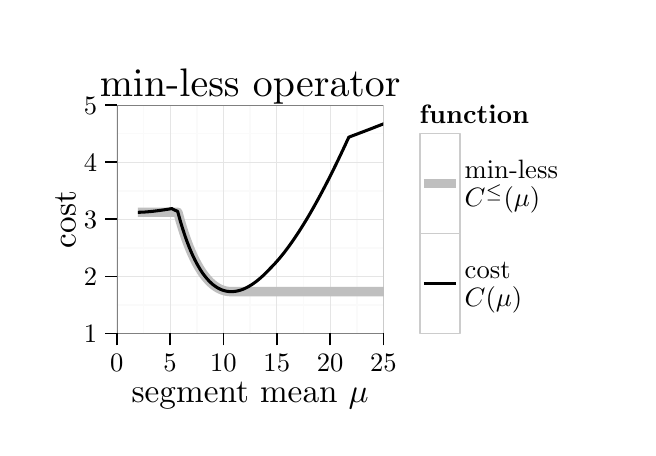
\begin{tikzpicture}[x=1pt,y=1pt]
\definecolor[named]{fillColor}{rgb}{1.00,1.00,1.00}
\path[use as bounding box,fill=fillColor,fill opacity=0.00] (0,0) rectangle (216.81,144.54);
\begin{scope}
\path[clip] (  0.00,  0.00) rectangle (216.81,144.54);
\definecolor[named]{drawColor}{rgb}{1.00,1.00,1.00}
\definecolor[named]{fillColor}{rgb}{1.00,1.00,1.00}

\path[draw=drawColor,line width= 0.6pt,line join=round,line cap=round,fill=fillColor] ( -0.00,  0.00) rectangle (216.81,144.54);
\end{scope}
\begin{scope}
\path[clip] ( 32.22, 34.03) rectangle (128.53,116.55);
\definecolor[named]{fillColor}{rgb}{1.00,1.00,1.00}

\path[fill=fillColor] ( 32.22, 34.03) rectangle (128.53,116.55);
\definecolor[named]{drawColor}{rgb}{0.98,0.98,0.98}

\path[draw=drawColor,line width= 0.6pt,line join=round] ( 32.22, 44.35) --
	(128.53, 44.35);

\path[draw=drawColor,line width= 0.6pt,line join=round] ( 32.22, 64.98) --
	(128.53, 64.98);

\path[draw=drawColor,line width= 0.6pt,line join=round] ( 32.22, 85.61) --
	(128.53, 85.61);

\path[draw=drawColor,line width= 0.6pt,line join=round] ( 32.22,106.24) --
	(128.53,106.24);

\path[draw=drawColor,line width= 0.6pt,line join=round] ( 41.85, 34.03) --
	( 41.85,116.55);

\path[draw=drawColor,line width= 0.6pt,line join=round] ( 61.12, 34.03) --
	( 61.12,116.55);

\path[draw=drawColor,line width= 0.6pt,line join=round] ( 80.38, 34.03) --
	( 80.38,116.55);

\path[draw=drawColor,line width= 0.6pt,line join=round] ( 99.64, 34.03) --
	( 99.64,116.55);

\path[draw=drawColor,line width= 0.6pt,line join=round] (118.90, 34.03) --
	(118.90,116.55);
\definecolor[named]{drawColor}{rgb}{0.90,0.90,0.90}

\path[draw=drawColor,line width= 0.2pt,line join=round] ( 32.22, 34.03) --
	(128.53, 34.03);

\path[draw=drawColor,line width= 0.2pt,line join=round] ( 32.22, 54.66) --
	(128.53, 54.66);

\path[draw=drawColor,line width= 0.2pt,line join=round] ( 32.22, 75.29) --
	(128.53, 75.29);

\path[draw=drawColor,line width= 0.2pt,line join=round] ( 32.22, 95.92) --
	(128.53, 95.92);

\path[draw=drawColor,line width= 0.2pt,line join=round] ( 32.22,116.55) --
	(128.53,116.55);

\path[draw=drawColor,line width= 0.2pt,line join=round] ( 32.22, 34.03) --
	( 32.22,116.55);

\path[draw=drawColor,line width= 0.2pt,line join=round] ( 51.48, 34.03) --
	( 51.48,116.55);

\path[draw=drawColor,line width= 0.2pt,line join=round] ( 70.75, 34.03) --
	( 70.75,116.55);

\path[draw=drawColor,line width= 0.2pt,line join=round] ( 90.01, 34.03) --
	( 90.01,116.55);

\path[draw=drawColor,line width= 0.2pt,line join=round] (109.27, 34.03) --
	(109.27,116.55);

\path[draw=drawColor,line width= 0.2pt,line join=round] (128.53, 34.03) --
	(128.53,116.55);
\definecolor[named]{drawColor}{rgb}{0.75,0.75,0.75}

\path[draw=drawColor,line width= 3.4pt,line join=round] ( 39.81, 77.83) --
	( 39.96, 77.83) --
	( 40.10, 77.83) --
	( 40.25, 77.83) --
	( 40.40, 77.83) --
	( 40.54, 77.83) --
	( 40.69, 77.83) --
	( 40.83, 77.83) --
	( 40.98, 77.83) --
	( 41.13, 77.83) --
	( 41.27, 77.83) --
	( 41.42, 77.83) --
	( 41.56, 77.83) --
	( 41.71, 77.83) --
	( 41.86, 77.83) --
	( 42.00, 77.83) --
	( 42.15, 77.83) --
	( 42.30, 77.83) --
	( 42.44, 77.83) --
	( 42.59, 77.83) --
	( 42.73, 77.83) --
	( 42.88, 77.83) --
	( 43.03, 77.83) --
	( 43.17, 77.83) --
	( 43.32, 77.83) --
	( 43.46, 77.83) --
	( 43.61, 77.83) --
	( 43.76, 77.83) --
	( 43.90, 77.83) --
	( 44.05, 77.83) --
	( 44.20, 77.83) --
	( 44.34, 77.83) --
	( 44.49, 77.83) --
	( 44.63, 77.83) --
	( 44.78, 77.83) --
	( 44.93, 77.83) --
	( 45.07, 77.83) --
	( 45.22, 77.83) --
	( 45.37, 77.83) --
	( 45.51, 77.83) --
	( 45.66, 77.83) --
	( 45.80, 77.83) --
	( 45.95, 77.83) --
	( 46.10, 77.83) --
	( 46.24, 77.83) --
	( 46.39, 77.83) --
	( 46.53, 77.83) --
	( 46.68, 77.83) --
	( 46.83, 77.83) --
	( 46.97, 77.83) --
	( 47.12, 77.83) --
	( 47.27, 77.83) --
	( 47.41, 77.83) --
	( 47.56, 77.83) --
	( 47.70, 77.83) --
	( 47.85, 77.83) --
	( 48.00, 77.83) --
	( 48.14, 77.83) --
	( 48.29, 77.83) --
	( 48.43, 77.83) --
	( 48.58, 77.83) --
	( 48.73, 77.83) --
	( 48.87, 77.83) --
	( 49.02, 77.83) --
	( 49.17, 77.83) --
	( 49.31, 77.83) --
	( 49.46, 77.83) --
	( 49.60, 77.83) --
	( 49.75, 77.83) --
	( 49.90, 77.83) --
	( 50.04, 77.83) --
	( 50.19, 77.83) --
	( 50.33, 77.83) --
	( 50.48, 77.83) --
	( 50.63, 77.83) --
	( 50.77, 77.83) --
	( 50.92, 77.83) --
	( 51.07, 77.83) --
	( 51.21, 77.83) --
	( 51.36, 77.83) --
	( 51.50, 77.83) --
	( 51.65, 77.83) --
	( 51.80, 77.83) --
	( 51.94, 77.83) --
	( 52.09, 77.83) --
	( 52.23, 77.83) --
	( 52.38, 77.83) --
	( 52.53, 77.83) --
	( 52.67, 77.83) --
	( 52.82, 77.83) --
	( 52.97, 77.83) --
	( 53.11, 77.83) --
	( 53.26, 77.83) --
	( 53.40, 77.83) --
	( 53.55, 77.83) --
	( 53.70, 77.83) --
	( 53.84, 77.83) --
	( 53.99, 77.83) --
	( 54.13, 77.83) --
	( 54.28, 77.83) --
	( 54.28, 77.83) --
	( 54.48, 77.11) --
	( 54.67, 76.40) --
	( 54.87, 75.70) --
	( 55.06, 75.02) --
	( 55.25, 74.35) --
	( 55.45, 73.69) --
	( 55.64, 73.05) --
	( 55.84, 72.41) --
	( 56.03, 71.79) --
	( 56.23, 71.18) --
	( 56.42, 70.58) --
	( 56.62, 70.00) --
	( 56.81, 69.42) --
	( 57.01, 68.86) --
	( 57.20, 68.31) --
	( 57.40, 67.77) --
	( 57.59, 67.24) --
	( 57.79, 66.72) --
	( 57.98, 66.20) --
	( 58.18, 65.70) --
	( 58.37, 65.21) --
	( 58.57, 64.73) --
	( 58.76, 64.26) --
	( 58.96, 63.80) --
	( 59.15, 63.35) --
	( 59.35, 62.91) --
	( 59.54, 62.47) --
	( 59.74, 62.05) --
	( 59.93, 61.64) --
	( 60.13, 61.23) --
	( 60.32, 60.83) --
	( 60.52, 60.44) --
	( 60.71, 60.06) --
	( 60.91, 59.69) --
	( 61.10, 59.32) --
	( 61.30, 58.97) --
	( 61.49, 58.62) --
	( 61.69, 58.28) --
	( 61.88, 57.94) --
	( 62.08, 57.62) --
	( 62.27, 57.30) --
	( 62.47, 56.99) --
	( 62.66, 56.69) --
	( 62.86, 56.39) --
	( 63.05, 56.10) --
	( 63.24, 55.82) --
	( 63.44, 55.55) --
	( 63.63, 55.28) --
	( 63.83, 55.02) --
	( 64.02, 54.77) --
	( 64.22, 54.52) --
	( 64.41, 54.28) --
	( 64.61, 54.04) --
	( 64.80, 53.81) --
	( 65.00, 53.59) --
	( 65.19, 53.38) --
	( 65.39, 53.17) --
	( 65.58, 52.97) --
	( 65.78, 52.77) --
	( 65.97, 52.58) --
	( 66.17, 52.39) --
	( 66.36, 52.21) --
	( 66.56, 52.04) --
	( 66.75, 51.87) --
	( 66.95, 51.71) --
	( 67.14, 51.55) --
	( 67.34, 51.40) --
	( 67.53, 51.26) --
	( 67.73, 51.12) --
	( 67.92, 50.98) --
	( 68.12, 50.85) --
	( 68.31, 50.73) --
	( 68.51, 50.61) --
	( 68.70, 50.50) --
	( 68.90, 50.39) --
	( 69.09, 50.28) --
	( 69.29, 50.18) --
	( 69.48, 50.09) --
	( 69.68, 50.00) --
	( 69.87, 49.92) --
	( 70.07, 49.84) --
	( 70.26, 49.76) --
	( 70.46, 49.69) --
	( 70.65, 49.62) --
	( 70.85, 49.56) --
	( 71.04, 49.51) --
	( 71.23, 49.45) --
	( 71.43, 49.41) --
	( 71.62, 49.36) --
	( 71.82, 49.32) --
	( 72.01, 49.29) --
	( 72.21, 49.26) --
	( 72.40, 49.23) --
	( 72.60, 49.21) --
	( 72.79, 49.19) --
	( 72.99, 49.18) --
	( 73.18, 49.17) --
	( 73.38, 49.16) --
	( 73.57, 49.16) --
	( 73.57, 49.16) --
	( 81.49, 49.16) --
	( 89.41, 49.16) --
	( 97.33, 49.16) --
	(105.25, 49.16) --
	(113.17, 49.16) --
	(121.09, 49.16) --
	(129.01, 49.16) --
	(136.93, 49.16) --
	(144.85, 49.16) --
	(152.77, 49.16) --
	(160.69, 49.16) --
	(168.60, 49.16) --
	(176.52, 49.16) --
	(184.44, 49.16) --
	(192.36, 49.16) --
	(200.28, 49.16) --
	(208.20, 49.16) --
	(216.12, 49.16) --
	(216.81, 49.16);
\definecolor[named]{drawColor}{rgb}{0.00,0.00,0.00}

\path[draw=drawColor,line width= 1.1pt,line join=round] ( 39.81, 77.83) --
	( 39.94, 77.83) --
	( 40.06, 77.83) --
	( 40.18, 77.83) --
	( 40.31, 77.84) --
	( 40.43, 77.84) --
	( 40.55, 77.84) --
	( 40.68, 77.84) --
	( 40.80, 77.85) --
	( 40.93, 77.85) --
	( 41.05, 77.86) --
	( 41.17, 77.86) --
	( 41.30, 77.87) --
	( 41.42, 77.87) --
	( 41.55, 77.88) --
	( 41.67, 77.88) --
	( 41.79, 77.89) --
	( 41.92, 77.90) --
	( 42.04, 77.90) --
	( 42.17, 77.91) --
	( 42.29, 77.92) --
	( 42.41, 77.93) --
	( 42.54, 77.94) --
	( 42.66, 77.95) --
	( 42.79, 77.96) --
	( 42.91, 77.96) --
	( 43.03, 77.97) --
	( 43.16, 77.98) --
	( 43.28, 77.99) --
	( 43.41, 78.01) --
	( 43.53, 78.02) --
	( 43.65, 78.03) --
	( 43.78, 78.04) --
	( 43.90, 78.05) --
	( 44.03, 78.06) --
	( 44.15, 78.07) --
	( 44.27, 78.09) --
	( 44.40, 78.10) --
	( 44.52, 78.11) --
	( 44.65, 78.12) --
	( 44.77, 78.14) --
	( 44.89, 78.15) --
	( 45.02, 78.16) --
	( 45.14, 78.18) --
	( 45.26, 78.19) --
	( 45.39, 78.20) --
	( 45.51, 78.22) --
	( 45.64, 78.23) --
	( 45.76, 78.25) --
	( 45.88, 78.26) --
	( 46.01, 78.28) --
	( 46.13, 78.29) --
	( 46.26, 78.31) --
	( 46.38, 78.32) --
	( 46.50, 78.34) --
	( 46.63, 78.35) --
	( 46.75, 78.37) --
	( 46.88, 78.39) --
	( 47.00, 78.40) --
	( 47.12, 78.42) --
	( 47.25, 78.43) --
	( 47.37, 78.45) --
	( 47.50, 78.47) --
	( 47.62, 78.48) --
	( 47.74, 78.50) --
	( 47.87, 78.52) --
	( 47.99, 78.54) --
	( 48.12, 78.55) --
	( 48.24, 78.57) --
	( 48.36, 78.59) --
	( 48.49, 78.60) --
	( 48.61, 78.62) --
	( 48.74, 78.64) --
	( 48.86, 78.66) --
	( 48.98, 78.68) --
	( 49.11, 78.69) --
	( 49.23, 78.71) --
	( 49.36, 78.73) --
	( 49.48, 78.75) --
	( 49.60, 78.77) --
	( 49.73, 78.79) --
	( 49.85, 78.81) --
	( 49.98, 78.83) --
	( 50.10, 78.84) --
	( 50.22, 78.86) --
	( 50.35, 78.88) --
	( 50.47, 78.90) --
	( 50.59, 78.92) --
	( 50.72, 78.94) --
	( 50.84, 78.96) --
	( 50.97, 78.98) --
	( 51.09, 79.00) --
	( 51.21, 79.02) --
	( 51.34, 79.04) --
	( 51.46, 79.06) --
	( 51.59, 79.08) --
	( 51.71, 79.10) --
	( 51.83, 79.12) --
	( 51.96, 79.14) --
	( 52.08, 79.16) --
	( 52.08, 79.16) --
	( 52.10, 79.15) --
	( 52.12, 79.14) --
	( 52.15, 79.13) --
	( 52.17, 79.12) --
	( 52.19, 79.10) --
	( 52.21, 79.09) --
	( 52.23, 79.08) --
	( 52.25, 79.07) --
	( 52.27, 79.06) --
	( 52.30, 79.05) --
	( 52.32, 79.04) --
	( 52.34, 79.02) --
	( 52.36, 79.01) --
	( 52.38, 79.00) --
	( 52.40, 78.99) --
	( 52.42, 78.98) --
	( 52.44, 78.97) --
	( 52.47, 78.96) --
	( 52.49, 78.95) --
	( 52.51, 78.93) --
	( 52.53, 78.92) --
	( 52.55, 78.91) --
	( 52.57, 78.90) --
	( 52.59, 78.89) --
	( 52.61, 78.88) --
	( 52.64, 78.87) --
	( 52.66, 78.86) --
	( 52.68, 78.85) --
	( 52.70, 78.84) --
	( 52.72, 78.83) --
	( 52.74, 78.82) --
	( 52.76, 78.81) --
	( 52.78, 78.80) --
	( 52.81, 78.78) --
	( 52.83, 78.77) --
	( 52.85, 78.76) --
	( 52.87, 78.75) --
	( 52.89, 78.74) --
	( 52.91, 78.73) --
	( 52.93, 78.72) --
	( 52.96, 78.71) --
	( 52.98, 78.70) --
	( 53.00, 78.69) --
	( 53.02, 78.68) --
	( 53.04, 78.67) --
	( 53.06, 78.66) --
	( 53.08, 78.65) --
	( 53.10, 78.64) --
	( 53.13, 78.63) --
	( 53.15, 78.62) --
	( 53.17, 78.61) --
	( 53.19, 78.60) --
	( 53.21, 78.59) --
	( 53.23, 78.58) --
	( 53.25, 78.57) --
	( 53.27, 78.56) --
	( 53.30, 78.55) --
	( 53.32, 78.54) --
	( 53.34, 78.53) --
	( 53.36, 78.52) --
	( 53.38, 78.51) --
	( 53.40, 78.50) --
	( 53.42, 78.49) --
	( 53.44, 78.48) --
	( 53.47, 78.48) --
	( 53.49, 78.47) --
	( 53.51, 78.46) --
	( 53.53, 78.45) --
	( 53.55, 78.44) --
	( 53.57, 78.43) --
	( 53.59, 78.42) --
	( 53.62, 78.41) --
	( 53.64, 78.40) --
	( 53.66, 78.39) --
	( 53.68, 78.38) --
	( 53.70, 78.37) --
	( 53.72, 78.36) --
	( 53.74, 78.36) --
	( 53.76, 78.35) --
	( 53.79, 78.34) --
	( 53.81, 78.33) --
	( 53.83, 78.32) --
	( 53.85, 78.31) --
	( 53.87, 78.30) --
	( 53.89, 78.29) --
	( 53.91, 78.28) --
	( 53.93, 78.27) --
	( 53.96, 78.27) --
	( 53.98, 78.26) --
	( 54.00, 78.25) --
	( 54.02, 78.24) --
	( 54.04, 78.23) --
	( 54.06, 78.22) --
	( 54.08, 78.21) --
	( 54.10, 78.21) --
	( 54.13, 78.20) --
	( 54.15, 78.19) --
	( 54.17, 78.18) --
	( 54.19, 78.17) --
	( 54.19, 78.17) --
	( 54.53, 76.92) --
	( 54.87, 75.70) --
	( 55.20, 74.52) --
	( 55.54, 73.38) --
	( 55.88, 72.28) --
	( 56.22, 71.22) --
	( 56.56, 70.19) --
	( 56.89, 69.19) --
	( 57.23, 68.23) --
	( 57.57, 67.30) --
	( 57.91, 66.40) --
	( 58.24, 65.54) --
	( 58.58, 64.70) --
	( 58.92, 63.89) --
	( 59.26, 63.11) --
	( 59.60, 62.36) --
	( 59.93, 61.63) --
	( 60.27, 60.93) --
	( 60.61, 60.26) --
	( 60.95, 59.61) --
	( 61.29, 58.98) --
	( 61.62, 58.38) --
	( 61.96, 57.81) --
	( 62.30, 57.25) --
	( 62.64, 56.72) --
	( 62.98, 56.21) --
	( 63.31, 55.72) --
	( 63.65, 55.26) --
	( 63.99, 54.81) --
	( 64.33, 54.38) --
	( 64.67, 53.98) --
	( 65.00, 53.59) --
	( 65.34, 53.22) --
	( 65.68, 52.87) --
	( 66.02, 52.54) --
	( 66.35, 52.22) --
	( 66.69, 51.92) --
	( 67.03, 51.64) --
	( 67.37, 51.38) --
	( 67.71, 51.13) --
	( 68.04, 50.90) --
	( 68.38, 50.68) --
	( 68.72, 50.48) --
	( 69.06, 50.30) --
	( 69.40, 50.13) --
	( 69.73, 49.97) --
	( 70.07, 49.83) --
	( 70.41, 49.71) --
	( 70.75, 49.59) --
	( 71.09, 49.49) --
	( 71.42, 49.41) --
	( 71.76, 49.34) --
	( 72.10, 49.28) --
	( 72.44, 49.23) --
	( 72.78, 49.19) --
	( 73.11, 49.17) --
	( 73.45, 49.16) --
	( 73.79, 49.16) --
	( 74.13, 49.18) --
	( 74.46, 49.20) --
	( 74.80, 49.24) --
	( 75.14, 49.28) --
	( 75.48, 49.34) --
	( 75.82, 49.41) --
	( 76.15, 49.49) --
	( 76.49, 49.58) --
	( 76.83, 49.68) --
	( 77.17, 49.79) --
	( 77.51, 49.91) --
	( 77.84, 50.04) --
	( 78.18, 50.18) --
	( 78.52, 50.33) --
	( 78.86, 50.49) --
	( 79.20, 50.66) --
	( 79.53, 50.84) --
	( 79.87, 51.03) --
	( 80.21, 51.22) --
	( 80.55, 51.43) --
	( 80.89, 51.64) --
	( 81.22, 51.86) --
	( 81.56, 52.09) --
	( 81.90, 52.33) --
	( 82.24, 52.58) --
	( 82.57, 52.83) --
	( 82.91, 53.10) --
	( 83.25, 53.37) --
	( 83.59, 53.64) --
	( 83.93, 53.93) --
	( 84.26, 54.22) --
	( 84.60, 54.53) --
	( 84.94, 54.83) --
	( 85.28, 55.15) --
	( 85.62, 55.47) --
	( 85.95, 55.80) --
	( 86.29, 56.14) --
	( 86.63, 56.48) --
	( 86.97, 56.83) --
	( 87.31, 57.19) --
	( 87.64, 57.56) --
	( 87.64, 57.56) --
	( 87.93, 57.84) --
	( 88.22, 58.13) --
	( 88.50, 58.43) --
	( 88.79, 58.73) --
	( 89.08, 59.03) --
	( 89.36, 59.34) --
	( 89.65, 59.66) --
	( 89.94, 59.98) --
	( 90.22, 60.30) --
	( 90.51, 60.63) --
	( 90.80, 60.96) --
	( 91.09, 61.30) --
	( 91.37, 61.65) --
	( 91.66, 62.00) --
	( 91.95, 62.35) --
	( 92.23, 62.71) --
	( 92.52, 63.07) --
	( 92.81, 63.44) --
	( 93.09, 63.81) --
	( 93.38, 64.18) --
	( 93.67, 64.56) --
	( 93.95, 64.95) --
	( 94.24, 65.34) --
	( 94.53, 65.73) --
	( 94.81, 66.13) --
	( 95.10, 66.53) --
	( 95.39, 66.93) --
	( 95.67, 67.34) --
	( 95.96, 67.76) --
	( 96.25, 68.17) --
	( 96.53, 68.59) --
	( 96.82, 69.02) --
	( 97.11, 69.45) --
	( 97.39, 69.88) --
	( 97.68, 70.32) --
	( 97.97, 70.76) --
	( 98.25, 71.20) --
	( 98.54, 71.65) --
	( 98.83, 72.10) --
	( 99.11, 72.56) --
	( 99.40, 73.02) --
	( 99.69, 73.48) --
	( 99.98, 73.95) --
	(100.26, 74.42) --
	(100.55, 74.89) --
	(100.84, 75.37) --
	(101.12, 75.85) --
	(101.41, 76.33) --
	(101.70, 76.82) --
	(101.98, 77.31) --
	(102.27, 77.80) --
	(102.56, 78.30) --
	(102.84, 78.80) --
	(103.13, 79.31) --
	(103.42, 79.81) --
	(103.70, 80.32) --
	(103.99, 80.84) --
	(104.28, 81.35) --
	(104.56, 81.87) --
	(104.85, 82.39) --
	(105.14, 82.92) --
	(105.42, 83.45) --
	(105.71, 83.98) --
	(106.00, 84.52) --
	(106.28, 85.05) --
	(106.57, 85.60) --
	(106.86, 86.14) --
	(107.14, 86.69) --
	(107.43, 87.24) --
	(107.72, 87.79) --
	(108.01, 88.34) --
	(108.29, 88.90) --
	(108.58, 89.46) --
	(108.87, 90.03) --
	(109.15, 90.59) --
	(109.44, 91.16) --
	(109.73, 91.73) --
	(110.01, 92.31) --
	(110.30, 92.89) --
	(110.59, 93.47) --
	(110.87, 94.05) --
	(111.16, 94.64) --
	(111.45, 95.22) --
	(111.73, 95.81) --
	(112.02, 96.41) --
	(112.31, 97.00) --
	(112.59, 97.60) --
	(112.88, 98.20) --
	(113.17, 98.81) --
	(113.45, 99.41) --
	(113.74,100.02) --
	(114.03,100.63) --
	(114.31,101.24) --
	(114.60,101.86) --
	(114.89,102.48) --
	(115.17,103.10) --
	(115.46,103.72) --
	(115.75,104.34) --
	(116.04,104.97) --
	(116.04,104.97) --
	(123.53,107.81) --
	(131.02,110.74) --
	(138.51,113.74) --
	(146.00,116.82) --
	(153.49,119.96) --
	(160.98,123.14) --
	(168.47,126.38) --
	(175.96,129.66) --
	(183.45,132.97) --
	(190.94,136.32) --
	(198.43,139.69) --
	(205.92,143.10) --
	(209.06,144.54);
\definecolor[named]{drawColor}{rgb}{0.50,0.50,0.50}

\path[draw=drawColor,line width= 0.6pt,line join=round,line cap=round] ( 32.22, 34.03) rectangle (128.53,116.55);
\end{scope}
\begin{scope}
\path[clip] (  0.00,  0.00) rectangle (216.81,144.54);
\definecolor[named]{drawColor}{rgb}{0.00,0.00,0.00}

\node[text=drawColor,anchor=base east,inner sep=0pt, outer sep=0pt, scale=  0.96] at ( 25.11, 30.73) {1};

\node[text=drawColor,anchor=base east,inner sep=0pt, outer sep=0pt, scale=  0.96] at ( 25.11, 51.36) {2};

\node[text=drawColor,anchor=base east,inner sep=0pt, outer sep=0pt, scale=  0.96] at ( 25.11, 71.99) {3};

\node[text=drawColor,anchor=base east,inner sep=0pt, outer sep=0pt, scale=  0.96] at ( 25.11, 92.62) {4};

\node[text=drawColor,anchor=base east,inner sep=0pt, outer sep=0pt, scale=  0.96] at ( 25.11,113.25) {5};
\end{scope}
\begin{scope}
\path[clip] (  0.00,  0.00) rectangle (216.81,144.54);
\definecolor[named]{drawColor}{rgb}{0.00,0.00,0.00}

\path[draw=drawColor,line width= 0.6pt,line join=round] ( 27.95, 34.03) --
	( 32.22, 34.03);

\path[draw=drawColor,line width= 0.6pt,line join=round] ( 27.95, 54.66) --
	( 32.22, 54.66);

\path[draw=drawColor,line width= 0.6pt,line join=round] ( 27.95, 75.29) --
	( 32.22, 75.29);

\path[draw=drawColor,line width= 0.6pt,line join=round] ( 27.95, 95.92) --
	( 32.22, 95.92);

\path[draw=drawColor,line width= 0.6pt,line join=round] ( 27.95,116.55) --
	( 32.22,116.55);
\end{scope}
\begin{scope}
\path[clip] (  0.00,  0.00) rectangle (216.81,144.54);
\definecolor[named]{drawColor}{rgb}{0.00,0.00,0.00}

\path[draw=drawColor,line width= 0.6pt,line join=round] ( 32.22, 29.77) --
	( 32.22, 34.03);

\path[draw=drawColor,line width= 0.6pt,line join=round] ( 51.48, 29.77) --
	( 51.48, 34.03);

\path[draw=drawColor,line width= 0.6pt,line join=round] ( 70.75, 29.77) --
	( 70.75, 34.03);

\path[draw=drawColor,line width= 0.6pt,line join=round] ( 90.01, 29.77) --
	( 90.01, 34.03);

\path[draw=drawColor,line width= 0.6pt,line join=round] (109.27, 29.77) --
	(109.27, 34.03);

\path[draw=drawColor,line width= 0.6pt,line join=round] (128.53, 29.77) --
	(128.53, 34.03);
\end{scope}
\begin{scope}
\path[clip] (  0.00,  0.00) rectangle (216.81,144.54);
\definecolor[named]{drawColor}{rgb}{0.00,0.00,0.00}

\node[text=drawColor,anchor=base,inner sep=0pt, outer sep=0pt, scale=  0.96] at ( 32.22, 20.31) {0};

\node[text=drawColor,anchor=base,inner sep=0pt, outer sep=0pt, scale=  0.96] at ( 51.48, 20.31) {5};

\node[text=drawColor,anchor=base,inner sep=0pt, outer sep=0pt, scale=  0.96] at ( 70.75, 20.31) {10};

\node[text=drawColor,anchor=base,inner sep=0pt, outer sep=0pt, scale=  0.96] at ( 90.01, 20.31) {15};

\node[text=drawColor,anchor=base,inner sep=0pt, outer sep=0pt, scale=  0.96] at (109.27, 20.31) {20};

\node[text=drawColor,anchor=base,inner sep=0pt, outer sep=0pt, scale=  0.96] at (128.53, 20.31) {25};
\end{scope}
\begin{scope}
\path[clip] (  0.00,  0.00) rectangle (216.81,144.54);
\definecolor[named]{drawColor}{rgb}{0.00,0.00,0.00}

\node[text=drawColor,anchor=base,inner sep=0pt, outer sep=0pt, scale=  1.20] at ( 80.38,  9.03) {segment mean $\mu$};
\end{scope}
\begin{scope}
\path[clip] (  0.00,  0.00) rectangle (216.81,144.54);
\definecolor[named]{drawColor}{rgb}{0.00,0.00,0.00}

\node[text=drawColor,rotate= 90.00,anchor=base,inner sep=0pt, outer sep=0pt, scale=  1.20] at ( 17.30, 75.29) {cost};
\end{scope}
\begin{scope}
\path[clip] (  0.00,  0.00) rectangle (216.81,144.54);
\definecolor[named]{fillColor}{rgb}{1.00,1.00,1.00}

\path[fill=fillColor] (137.40, 29.77) rectangle (195.90,120.82);
\end{scope}
\begin{scope}
\path[clip] (  0.00,  0.00) rectangle (216.81,144.54);
\definecolor[named]{drawColor}{rgb}{0.00,0.00,0.00}

\node[text=drawColor,anchor=base west,inner sep=0pt, outer sep=0pt, scale=  0.96] at (141.67,109.92) {\bfseries function};
\end{scope}
\begin{scope}
\path[clip] (  0.00,  0.00) rectangle (216.81,144.54);
\definecolor[named]{drawColor}{rgb}{0.80,0.80,0.80}
\definecolor[named]{fillColor}{rgb}{1.00,1.00,1.00}

\path[draw=drawColor,line width= 0.6pt,line join=round,line cap=round,fill=fillColor] (141.67, 70.18) rectangle (156.12,106.31);
\end{scope}
\begin{scope}
\path[clip] (  0.00,  0.00) rectangle (216.81,144.54);
\definecolor[named]{drawColor}{rgb}{0.75,0.75,0.75}

\path[draw=drawColor,line width= 3.4pt,line join=round] (143.12, 88.24) -- (154.68, 88.24);
\end{scope}
\begin{scope}
\path[clip] (  0.00,  0.00) rectangle (216.81,144.54);
\definecolor[named]{drawColor}{rgb}{0.80,0.80,0.80}
\definecolor[named]{fillColor}{rgb}{1.00,1.00,1.00}

\path[draw=drawColor,line width= 0.6pt,line join=round,line cap=round,fill=fillColor] (141.67, 34.04) rectangle (156.12, 70.18);
\end{scope}
\begin{scope}
\path[clip] (  0.00,  0.00) rectangle (216.81,144.54);
\definecolor[named]{drawColor}{rgb}{0.00,0.00,0.00}

\path[draw=drawColor,line width= 1.1pt,line join=round] (143.12, 52.11) -- (154.68, 52.11);
\end{scope}
\begin{scope}
\path[clip] (  0.00,  0.00) rectangle (216.81,144.54);
\definecolor[named]{drawColor}{rgb}{0.00,0.00,0.00}

\node[text=drawColor,anchor=base west,inner sep=0pt, outer sep=0pt, scale=  0.96] at (157.93, 90.12) {min-less};

\node[text=drawColor,anchor=base west,inner sep=0pt, outer sep=0pt, scale=  0.96] at (157.93, 79.75) {$C^{\leq}(\mu)$};
\end{scope}
\begin{scope}
\path[clip] (  0.00,  0.00) rectangle (216.81,144.54);
\definecolor[named]{drawColor}{rgb}{0.00,0.00,0.00}

\node[text=drawColor,anchor=base west,inner sep=0pt, outer sep=0pt, scale=  0.96] at (157.93, 53.99) {cost};

\node[text=drawColor,anchor=base west,inner sep=0pt, outer sep=0pt, scale=  0.96] at (157.93, 43.62) {$C(\mu)$};
\end{scope}
\begin{scope}
\path[clip] (  0.00,  0.00) rectangle (216.81,144.54);
\definecolor[named]{drawColor}{rgb}{0.00,0.00,0.00}

\node[text=drawColor,anchor=base,inner sep=0pt, outer sep=0pt, scale=  1.44] at ( 80.38,119.57) {min-less operator};
\end{scope}
\end{tikzpicture}

    \end{center}
  }
  \caption{\label{fig:min-operators} \textbf{Left:} The min-more
    operator is $C^{\geq}(\mu)=\min_{x\geq \mu}C(x)$. \textbf{Right:}
    The min-less operator is $C^{\leq}(\mu)=\min_{x\leq
      \mu}C(x)$.}
\end{figure}

The next step is to compute the minimum cost in 2 segments up to data
point 3, for which there is a choice of two change-points.
\begin{equation*}
  C_{2,3}(\mu) = \min
  \begin{cases}
    C_{2,2}(\mu)+\gamma_3(\mu), \\
    C_{1,2}^{\leq}(\mu)+\gamma_3(\mu)
  \end{cases}
\end{equation*}
We have already computed an exact representation of the $C_{2,2}$
term, which is the cost a change after the first data point. Now we
need to compare it with the $C_{1,2}^{\leq}$ term, which is the cost
of a change after the second data point. This is a crucial step in
which the \texttt{MinEnvelope} sub-routine computes an exact
representation of the minimum of these two functions.

\begin{figure}[!t]
  \begin{center}
    % Created by tikzDevice version 0.12.3 on 2020-03-23 13:52:29
% !TEX encoding = UTF-8 Unicode
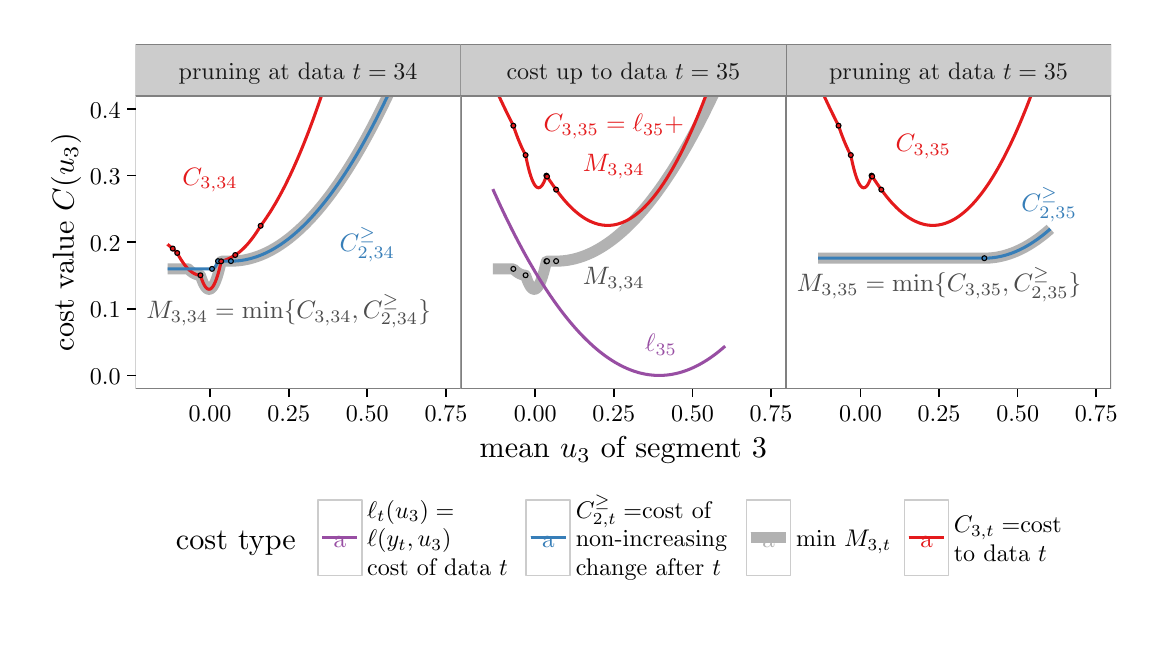
\begin{tikzpicture}[x=1pt,y=1pt]
\definecolor{fillColor}{RGB}{255,255,255}
\path[use as bounding box,fill=fillColor,fill opacity=0.00] (0,0) rectangle (397.48,216.81);
\begin{scope}
\path[clip] (  0.00,  0.00) rectangle (397.48,216.81);
\definecolor{drawColor}{RGB}{255,255,255}
\definecolor{fillColor}{RGB}{255,255,255}

\path[draw=drawColor,line width= 0.6pt,line join=round,line cap=round,fill=fillColor] (  0.00,  0.00) rectangle (397.48,216.81);
\end{scope}
\begin{scope}
\path[clip] ( 38.97,192.23) rectangle (156.48,210.81);
\definecolor{drawColor}{gray}{0.50}
\definecolor{fillColor}{gray}{0.80}

\path[draw=drawColor,line width= 0.2pt,line join=round,line cap=round,fill=fillColor] ( 38.97,192.23) rectangle (156.48,210.81);
\definecolor{drawColor}{gray}{0.10}

\node[text=drawColor,anchor=base,inner sep=0pt, outer sep=0pt, scale=  0.87] at ( 97.72,198.23) {pruning at data $t=34$};
\end{scope}
\begin{scope}
\path[clip] (156.48,192.23) rectangle (273.98,210.81);
\definecolor{drawColor}{gray}{0.50}
\definecolor{fillColor}{gray}{0.80}

\path[draw=drawColor,line width= 0.2pt,line join=round,line cap=round,fill=fillColor] (156.48,192.23) rectangle (273.98,210.81);
\definecolor{drawColor}{gray}{0.10}

\node[text=drawColor,anchor=base,inner sep=0pt, outer sep=0pt, scale=  0.87] at (215.23,198.23) {cost up to data $t=35$};
\end{scope}
\begin{scope}
\path[clip] (273.98,192.23) rectangle (391.48,210.81);
\definecolor{drawColor}{gray}{0.50}
\definecolor{fillColor}{gray}{0.80}

\path[draw=drawColor,line width= 0.2pt,line join=round,line cap=round,fill=fillColor] (273.98,192.23) rectangle (391.48,210.81);
\definecolor{drawColor}{gray}{0.10}

\node[text=drawColor,anchor=base,inner sep=0pt, outer sep=0pt, scale=  0.87] at (332.73,198.23) {pruning at data $t=35$};
\end{scope}
\begin{scope}
\path[clip] ( 38.97, 86.33) rectangle (156.48,192.23);
\definecolor{fillColor}{RGB}{255,255,255}

\path[fill=fillColor] ( 38.97, 86.33) rectangle (156.48,192.23);
\definecolor{drawColor}{gray}{0.70}

\path[draw=drawColor,line width= 4.0pt,line join=round] ( 50.58,129.65) --
	( 50.65,129.65) --
	( 50.73,129.65) --
	( 50.80,129.65) --
	( 50.88,129.65) --
	( 50.95,129.65) --
	( 51.02,129.65) --
	( 51.10,129.65) --
	( 51.17,129.65) --
	( 51.25,129.65) --
	( 51.32,129.65) --
	( 51.40,129.65) --
	( 51.47,129.65) --
	( 51.55,129.65) --
	( 51.62,129.65) --
	( 51.70,129.65) --
	( 51.77,129.65) --
	( 51.85,129.65) --
	( 51.92,129.65) --
	( 52.00,129.65) --
	( 52.07,129.65) --
	( 52.15,129.65) --
	( 52.22,129.65) --
	( 52.30,129.65) --
	( 52.37,129.65) --
	( 52.45,129.65) --
	( 52.52,129.65) --
	( 52.60,129.65) --
	( 52.67,129.65) --
	( 52.75,129.65) --
	( 52.82,129.65) --
	( 52.90,129.65) --
	( 52.97,129.65) --
	( 53.05,129.65) --
	( 53.12,129.65) --
	( 53.20,129.65) --
	( 53.27,129.65) --
	( 53.35,129.65) --
	( 53.42,129.65) --
	( 53.50,129.65) --
	( 53.57,129.65) --
	( 53.65,129.65) --
	( 53.72,129.65) --
	( 53.80,129.65) --
	( 53.87,129.65) --
	( 53.95,129.65) --
	( 54.02,129.65) --
	( 54.10,129.65) --
	( 54.17,129.65) --
	( 54.25,129.65) --
	( 54.32,129.65) --
	( 54.39,129.65) --
	( 54.47,129.65) --
	( 54.54,129.65) --
	( 54.62,129.65) --
	( 54.69,129.65) --
	( 54.77,129.65) --
	( 54.84,129.65) --
	( 54.92,129.65) --
	( 54.99,129.65) --
	( 55.07,129.65) --
	( 55.14,129.65) --
	( 55.22,129.65) --
	( 55.29,129.65) --
	( 55.37,129.65) --
	( 55.44,129.65) --
	( 55.52,129.65) --
	( 55.59,129.65) --
	( 55.67,129.65) --
	( 55.74,129.65) --
	( 55.82,129.65) --
	( 55.89,129.65) --
	( 55.97,129.65) --
	( 56.04,129.65) --
	( 56.12,129.65) --
	( 56.19,129.65) --
	( 56.27,129.65) --
	( 56.34,129.65) --
	( 56.42,129.65) --
	( 56.49,129.65) --
	( 56.57,129.65) --
	( 56.64,129.65) --
	( 56.72,129.65) --
	( 56.79,129.65) --
	( 56.87,129.65) --
	( 56.94,129.65) --
	( 57.02,129.65) --
	( 57.09,129.65) --
	( 57.17,129.65) --
	( 57.24,129.65) --
	( 57.32,129.65) --
	( 57.39,129.65) --
	( 57.47,129.65) --
	( 57.54,129.65) --
	( 57.61,129.65) --
	( 57.69,129.65) --
	( 57.76,129.65) --
	( 57.84,129.65) --
	( 57.91,129.65) --
	( 57.99,129.65) --
	( 57.99,129.65) --
	( 58.03,129.60) --
	( 58.08,129.56) --
	( 58.12,129.51) --
	( 58.17,129.47) --
	( 58.21,129.43) --
	( 58.26,129.38) --
	( 58.30,129.34) --
	( 58.35,129.30) --
	( 58.39,129.26) --
	( 58.44,129.21) --
	( 58.48,129.17) --
	( 58.53,129.13) --
	( 58.57,129.09) --
	( 58.62,129.05) --
	( 58.66,129.02) --
	( 58.71,128.98) --
	( 58.75,128.94) --
	( 58.79,128.90) --
	( 58.84,128.86) --
	( 58.88,128.83) --
	( 58.93,128.79) --
	( 58.97,128.76) --
	( 59.02,128.72) --
	( 59.06,128.69) --
	( 59.11,128.65) --
	( 59.15,128.62) --
	( 59.20,128.58) --
	( 59.24,128.55) --
	( 59.29,128.52) --
	( 59.33,128.49) --
	( 59.38,128.45) --
	( 59.42,128.42) --
	( 59.47,128.39) --
	( 59.51,128.36) --
	( 59.55,128.33) --
	( 59.60,128.30) --
	( 59.64,128.27) --
	( 59.69,128.24) --
	( 59.73,128.22) --
	( 59.78,128.19) --
	( 59.82,128.16) --
	( 59.87,128.13) --
	( 59.91,128.11) --
	( 59.96,128.08) --
	( 60.00,128.06) --
	( 60.05,128.03) --
	( 60.09,128.01) --
	( 60.14,127.98) --
	( 60.18,127.96) --
	( 60.23,127.94) --
	( 60.27,127.91) --
	( 60.32,127.89) --
	( 60.36,127.87) --
	( 60.40,127.85) --
	( 60.45,127.83) --
	( 60.49,127.81) --
	( 60.54,127.79) --
	( 60.58,127.77) --
	( 60.63,127.75) --
	( 60.67,127.73) --
	( 60.72,127.71) --
	( 60.76,127.69) --
	( 60.81,127.67) --
	( 60.85,127.66) --
	( 60.90,127.64) --
	( 60.94,127.62) --
	( 60.99,127.61) --
	( 61.03,127.59) --
	( 61.08,127.58) --
	( 61.12,127.57) --
	( 61.17,127.55) --
	( 61.21,127.54) --
	( 61.25,127.52) --
	( 61.30,127.51) --
	( 61.34,127.50) --
	( 61.39,127.49) --
	( 61.43,127.48) --
	( 61.48,127.47) --
	( 61.52,127.46) --
	( 61.57,127.45) --
	( 61.61,127.44) --
	( 61.66,127.43) --
	( 61.70,127.42) --
	( 61.75,127.41) --
	( 61.79,127.40) --
	( 61.84,127.40) --
	( 61.88,127.39) --
	( 61.93,127.38) --
	( 61.97,127.38) --
	( 62.02,127.37) --
	( 62.06,127.37) --
	( 62.10,127.36) --
	( 62.15,127.36) --
	( 62.19,127.36) --
	( 62.24,127.35) --
	( 62.28,127.35) --
	( 62.33,127.35) --
	( 62.37,127.35) --
	( 62.42,127.35) --
	( 62.42,127.35) --
	( 62.49,127.10) --
	( 62.57,126.86) --
	( 62.65,126.63) --
	( 62.72,126.41) --
	( 62.80,126.19) --
	( 62.87,125.97) --
	( 62.95,125.77) --
	( 63.03,125.56) --
	( 63.10,125.37) --
	( 63.18,125.18) --
	( 63.25,125.00) --
	( 63.33,124.82) --
	( 63.40,124.65) --
	( 63.48,124.48) --
	( 63.56,124.32) --
	( 63.63,124.17) --
	( 63.71,124.02) --
	( 63.78,123.88) --
	( 63.86,123.74) --
	( 63.94,123.61) --
	( 64.01,123.49) --
	( 64.09,123.37) --
	( 64.16,123.26) --
	( 64.24,123.16) --
	( 64.32,123.06) --
	( 64.39,122.96) --
	( 64.47,122.88) --
	( 64.54,122.80) --
	( 64.62,122.72) --
	( 64.69,122.65) --
	( 64.77,122.59) --
	( 64.85,122.53) --
	( 64.92,122.48) --
	( 65.00,122.43) --
	( 65.07,122.39) --
	( 65.15,122.36) --
	( 65.23,122.33) --
	( 65.30,122.31) --
	( 65.38,122.30) --
	( 65.45,122.29) --
	( 65.53,122.28) --
	( 65.61,122.29) --
	( 65.68,122.30) --
	( 65.76,122.31) --
	( 65.83,122.33) --
	( 65.91,122.36) --
	( 65.98,122.39) --
	( 66.06,122.43) --
	( 66.14,122.48) --
	( 66.21,122.53) --
	( 66.29,122.58) --
	( 66.36,122.65) --
	( 66.44,122.71) --
	( 66.52,122.79) --
	( 66.59,122.87) --
	( 66.67,122.96) --
	( 66.74,123.05) --
	( 66.82,123.15) --
	( 66.90,123.25) --
	( 66.97,123.37) --
	( 67.05,123.48) --
	( 67.12,123.61) --
	( 67.20,123.73) --
	( 67.28,123.87) --
	( 67.35,124.01) --
	( 67.43,124.16) --
	( 67.50,124.31) --
	( 67.58,124.47) --
	( 67.65,124.64) --
	( 67.73,124.81) --
	( 67.81,124.98) --
	( 67.88,125.17) --
	( 67.96,125.36) --
	( 68.03,125.55) --
	( 68.11,125.75) --
	( 68.19,125.96) --
	( 68.26,126.17) --
	( 68.34,126.39) --
	( 68.41,126.62) --
	( 68.49,126.85) --
	( 68.57,127.09) --
	( 68.64,127.33) --
	( 68.72,127.58) --
	( 68.79,127.83) --
	( 68.87,128.09) --
	( 68.94,128.36) --
	( 69.02,128.63) --
	( 69.10,128.91) --
	( 69.17,129.20) --
	( 69.25,129.49) --
	( 69.32,129.79) --
	( 69.40,130.09) --
	( 69.48,130.40) --
	( 69.55,130.72) --
	( 69.63,131.04) --
	( 69.70,131.36) --
	( 69.78,131.70) --
	( 69.86,132.04) --
	( 69.93,132.38) --
	( 69.93,132.38) --
	( 69.93,132.38) --
	( 69.94,132.38) --
	( 69.94,132.38) --
	( 69.94,132.39) --
	( 69.94,132.39) --
	( 69.95,132.39) --
	( 69.95,132.39) --
	( 69.95,132.39) --
	( 69.95,132.39) --
	( 69.96,132.39) --
	( 69.96,132.39) --
	( 69.96,132.39) --
	( 69.96,132.39) --
	( 69.96,132.39) --
	( 69.97,132.39) --
	( 69.97,132.39) --
	( 69.97,132.39) --
	( 69.97,132.39) --
	( 69.98,132.39) --
	( 69.98,132.40) --
	( 69.98,132.40) --
	( 69.98,132.40) --
	( 69.99,132.40) --
	( 69.99,132.40) --
	( 69.99,132.40) --
	( 69.99,132.40) --
	( 70.00,132.40) --
	( 70.00,132.40) --
	( 70.00,132.40) --
	( 70.00,132.40) --
	( 70.01,132.40) --
	( 70.01,132.40) --
	( 70.01,132.40) --
	( 70.01,132.40) --
	( 70.02,132.40) --
	( 70.02,132.41) --
	( 70.02,132.41) --
	( 70.02,132.41) --
	( 70.02,132.41) --
	( 70.03,132.41) --
	( 70.03,132.41) --
	( 70.03,132.41) --
	( 70.03,132.41) --
	( 70.04,132.41) --
	( 70.04,132.41) --
	( 70.04,132.41) --
	( 70.04,132.41) --
	( 70.05,132.41) --
	( 70.05,132.41) --
	( 70.05,132.41) --
	( 70.05,132.42) --
	( 70.06,132.42) --
	( 70.06,132.42) --
	( 70.06,132.42) --
	( 70.06,132.42) --
	( 70.07,132.42) --
	( 70.07,132.42) --
	( 70.07,132.42) --
	( 70.07,132.42) --
	( 70.08,132.42) --
	( 70.08,132.42) --
	( 70.08,132.42) --
	( 70.08,132.42) --
	( 70.08,132.42) --
	( 70.09,132.42) --
	( 70.09,132.42) --
	( 70.09,132.43) --
	( 70.09,132.43) --
	( 70.10,132.43) --
	( 70.10,132.43) --
	( 70.10,132.43) --
	( 70.10,132.43) --
	( 70.11,132.43) --
	( 70.11,132.43) --
	( 70.11,132.43) --
	( 70.11,132.43) --
	( 70.12,132.43) --
	( 70.12,132.43) --
	( 70.12,132.43) --
	( 70.12,132.43) --
	( 70.13,132.43) --
	( 70.13,132.44) --
	( 70.13,132.44) --
	( 70.13,132.44) --
	( 70.14,132.44) --
	( 70.14,132.44) --
	( 70.14,132.44) --
	( 70.14,132.44) --
	( 70.14,132.44) --
	( 70.15,132.44) --
	( 70.15,132.44) --
	( 70.15,132.44) --
	( 70.15,132.44) --
	( 70.16,132.44) --
	( 70.16,132.44) --
	( 70.16,132.44) --
	( 70.16,132.45) --
	( 70.17,132.45) --
	( 70.17,132.45) --
	( 70.17,132.45) --
	( 70.20,132.45) --
	( 70.24,132.45) --
	( 70.27,132.45) --
	( 70.30,132.45) --
	( 70.33,132.45) --
	( 70.37,132.45) --
	( 70.40,132.45) --
	( 70.43,132.45) --
	( 70.47,132.45) --
	( 70.50,132.45) --
	( 70.53,132.45) --
	( 70.57,132.45) --
	( 70.60,132.45) --
	( 70.63,132.45) --
	( 70.67,132.45) --
	( 70.70,132.45) --
	( 70.73,132.45) --
	( 70.77,132.45) --
	( 70.80,132.45) --
	( 70.83,132.45) --
	( 70.87,132.45) --
	( 70.90,132.45) --
	( 70.93,132.45) --
	( 70.96,132.45) --
	( 71.00,132.45) --
	( 71.03,132.45) --
	( 71.06,132.45) --
	( 71.10,132.45) --
	( 71.13,132.45) --
	( 71.16,132.45) --
	( 71.20,132.45) --
	( 71.23,132.45) --
	( 71.26,132.45) --
	( 71.30,132.45) --
	( 71.33,132.45) --
	( 71.36,132.45) --
	( 71.40,132.45) --
	( 71.43,132.45) --
	( 71.46,132.45) --
	( 71.50,132.45) --
	( 71.53,132.45) --
	( 71.56,132.45) --
	( 71.59,132.45) --
	( 71.63,132.45) --
	( 71.66,132.45) --
	( 71.69,132.45) --
	( 71.73,132.45) --
	( 71.76,132.45) --
	( 71.79,132.45) --
	( 71.83,132.45) --
	( 71.86,132.45) --
	( 71.89,132.45) --
	( 71.93,132.45) --
	( 71.96,132.45) --
	( 71.99,132.45) --
	( 72.03,132.45) --
	( 72.06,132.45) --
	( 72.09,132.45) --
	( 72.13,132.45) --
	( 72.16,132.45) --
	( 72.19,132.45) --
	( 72.23,132.45) --
	( 72.26,132.45) --
	( 72.29,132.45) --
	( 72.32,132.45) --
	( 72.36,132.45) --
	( 72.39,132.45) --
	( 72.42,132.45) --
	( 72.46,132.45) --
	( 72.49,132.45) --
	( 72.52,132.45) --
	( 72.56,132.45) --
	( 72.59,132.45) --
	( 72.62,132.45) --
	( 72.66,132.45) --
	( 72.69,132.45) --
	( 72.72,132.45) --
	( 72.76,132.45) --
	( 72.79,132.45) --
	( 72.82,132.45) --
	( 72.86,132.45) --
	( 72.89,132.45) --
	( 72.92,132.45) --
	( 72.95,132.45) --
	( 72.99,132.45) --
	( 73.02,132.45) --
	( 73.05,132.45) --
	( 73.09,132.45) --
	( 73.12,132.45) --
	( 73.15,132.45) --
	( 73.19,132.45) --
	( 73.22,132.45) --
	( 73.25,132.45) --
	( 73.29,132.45) --
	( 73.32,132.45) --
	( 73.35,132.45) --
	( 73.39,132.45) --
	( 73.42,132.45) --
	( 73.45,132.45) --
	( 73.45,132.45) --
	( 74.07,132.45) --
	( 74.69,132.47) --
	( 75.30,132.51) --
	( 75.92,132.56) --
	( 76.54,132.62) --
	( 77.15,132.70) --
	( 77.77,132.79) --
	( 78.39,132.90) --
	( 79.00,133.02) --
	( 79.62,133.16) --
	( 80.24,133.30) --
	( 80.85,133.47) --
	( 81.47,133.65) --
	( 82.09,133.84) --
	( 82.71,134.04) --
	( 83.32,134.26) --
	( 83.94,134.50) --
	( 84.56,134.74) --
	( 85.17,135.01) --
	( 85.79,135.28) --
	( 86.41,135.57) --
	( 87.02,135.88) --
	( 87.64,136.20) --
	( 88.26,136.53) --
	( 88.87,136.88) --
	( 89.49,137.24) --
	( 90.11,137.62) --
	( 90.73,138.01) --
	( 91.34,138.41) --
	( 91.96,138.83) --
	( 92.58,139.26) --
	( 93.19,139.71) --
	( 93.81,140.17) --
	( 94.43,140.64) --
	( 95.04,141.13) --
	( 95.66,141.64) --
	( 96.28,142.16) --
	( 96.89,142.69) --
	( 97.51,143.23) --
	( 98.13,143.79) --
	( 98.74,144.37) --
	( 99.36,144.96) --
	( 99.98,145.56) --
	(100.60,146.18) --
	(101.21,146.81) --
	(101.83,147.45) --
	(102.45,148.11) --
	(103.06,148.79) --
	(103.68,149.47) --
	(104.30,150.18) --
	(104.91,150.89) --
	(105.53,151.62) --
	(106.15,152.37) --
	(106.76,153.13) --
	(107.38,153.90) --
	(108.00,154.69) --
	(108.62,155.49) --
	(109.23,156.30) --
	(109.85,157.13) --
	(110.47,157.98) --
	(111.08,158.84) --
	(111.70,159.71) --
	(112.32,160.59) --
	(112.93,161.50) --
	(113.55,162.41) --
	(114.17,163.34) --
	(114.78,164.28) --
	(115.40,165.24) --
	(116.02,166.21) --
	(116.63,167.20) --
	(117.25,168.20) --
	(117.87,169.21) --
	(118.49,170.24) --
	(119.10,171.28) --
	(119.72,172.34) --
	(120.34,173.41) --
	(120.95,174.49) --
	(121.57,175.59) --
	(122.19,176.71) --
	(122.80,177.84) --
	(123.42,178.98) --
	(124.04,180.13) --
	(124.65,181.30) --
	(125.27,182.49) --
	(125.89,183.69) --
	(126.50,184.90) --
	(127.12,186.13) --
	(127.74,187.37) --
	(128.36,188.62) --
	(128.97,189.89) --
	(129.59,191.18) --
	(130.21,192.47) --
	(130.82,193.79) --
	(131.44,195.11) --
	(132.06,196.45) --
	(132.67,197.81) --
	(133.29,199.17) --
	(133.91,200.56) --
	(134.52,201.95);
\definecolor{drawColor}{RGB}{228,26,28}

\path[draw=drawColor,line width= 1.1pt,line join=round] ( 50.58,138.50) --
	( 50.59,138.48) --
	( 50.61,138.47) --
	( 50.63,138.45) --
	( 50.65,138.44) --
	( 50.67,138.42) --
	( 50.69,138.41) --
	( 50.71,138.39) --
	( 50.73,138.37) --
	( 50.74,138.36) --
	( 50.76,138.34) --
	( 50.78,138.33) --
	( 50.80,138.31) --
	( 50.82,138.29) --
	( 50.84,138.28) --
	( 50.86,138.26) --
	( 50.88,138.25) --
	( 50.89,138.23) --
	( 50.91,138.21) --
	( 50.93,138.20) --
	( 50.95,138.18) --
	( 50.97,138.17) --
	( 50.99,138.15) --
	( 51.01,138.14) --
	( 51.03,138.12) --
	( 51.04,138.10) --
	( 51.06,138.09) --
	( 51.08,138.07) --
	( 51.10,138.06) --
	( 51.12,138.04) --
	( 51.14,138.03) --
	( 51.16,138.01) --
	( 51.18,138.00) --
	( 51.20,137.98) --
	( 51.21,137.96) --
	( 51.23,137.95) --
	( 51.25,137.93) --
	( 51.27,137.92) --
	( 51.29,137.90) --
	( 51.31,137.89) --
	( 51.33,137.87) --
	( 51.35,137.86) --
	( 51.36,137.84) --
	( 51.38,137.82) --
	( 51.40,137.81) --
	( 51.42,137.79) --
	( 51.44,137.78) --
	( 51.46,137.76) --
	( 51.48,137.75) --
	( 51.50,137.73) --
	( 51.51,137.72) --
	( 51.53,137.70) --
	( 51.55,137.69) --
	( 51.57,137.67) --
	( 51.59,137.66) --
	( 51.61,137.64) --
	( 51.63,137.63) --
	( 51.65,137.61) --
	( 51.66,137.59) --
	( 51.68,137.58) --
	( 51.70,137.56) --
	( 51.72,137.55) --
	( 51.74,137.53) --
	( 51.76,137.52) --
	( 51.78,137.50) --
	( 51.80,137.49) --
	( 51.81,137.47) --
	( 51.83,137.46) --
	( 51.85,137.44) --
	( 51.87,137.43) --
	( 51.89,137.41) --
	( 51.91,137.40) --
	( 51.93,137.38) --
	( 51.95,137.37) --
	( 51.96,137.35) --
	( 51.98,137.34) --
	( 52.00,137.32) --
	( 52.02,137.31) --
	( 52.04,137.29) --
	( 52.06,137.28) --
	( 52.08,137.26) --
	( 52.10,137.25) --
	( 52.12,137.23) --
	( 52.13,137.22) --
	( 52.15,137.20) --
	( 52.17,137.19) --
	( 52.19,137.17) --
	( 52.21,137.16) --
	( 52.23,137.14) --
	( 52.25,137.13) --
	( 52.27,137.11) --
	( 52.28,137.10) --
	( 52.30,137.08) --
	( 52.32,137.07) --
	( 52.34,137.05) --
	( 52.36,137.04) --
	( 52.38,137.02) --
	( 52.40,137.01) --
	( 52.42,137.00) --
	( 52.43,136.98) --
	( 52.43,136.98) --
	( 52.45,136.96) --
	( 52.47,136.95) --
	( 52.48,136.93) --
	( 52.50,136.91) --
	( 52.52,136.90) --
	( 52.53,136.88) --
	( 52.55,136.86) --
	( 52.56,136.85) --
	( 52.58,136.83) --
	( 52.60,136.81) --
	( 52.61,136.80) --
	( 52.63,136.78) --
	( 52.65,136.76) --
	( 52.66,136.74) --
	( 52.68,136.73) --
	( 52.69,136.71) --
	( 52.71,136.69) --
	( 52.73,136.68) --
	( 52.74,136.66) --
	( 52.76,136.65) --
	( 52.78,136.63) --
	( 52.79,136.61) --
	( 52.81,136.60) --
	( 52.82,136.58) --
	( 52.84,136.56) --
	( 52.86,136.55) --
	( 52.87,136.53) --
	( 52.89,136.51) --
	( 52.90,136.50) --
	( 52.92,136.48) --
	( 52.94,136.46) --
	( 52.95,136.45) --
	( 52.97,136.43) --
	( 52.99,136.41) --
	( 53.00,136.40) --
	( 53.02,136.38) --
	( 53.03,136.37) --
	( 53.05,136.35) --
	( 53.07,136.33) --
	( 53.08,136.32) --
	( 53.10,136.30) --
	( 53.12,136.28) --
	( 53.13,136.27) --
	( 53.15,136.25) --
	( 53.16,136.24) --
	( 53.18,136.22) --
	( 53.20,136.20) --
	( 53.21,136.19) --
	( 53.23,136.17) --
	( 53.25,136.16) --
	( 53.26,136.14) --
	( 53.28,136.12) --
	( 53.29,136.11) --
	( 53.31,136.09) --
	( 53.33,136.08) --
	( 53.34,136.06) --
	( 53.36,136.04) --
	( 53.38,136.03) --
	( 53.39,136.01) --
	( 53.41,136.00) --
	( 53.42,135.98) --
	( 53.44,135.97) --
	( 53.46,135.95) --
	( 53.47,135.93) --
	( 53.49,135.92) --
	( 53.51,135.90) --
	( 53.52,135.89) --
	( 53.54,135.87) --
	( 53.55,135.86) --
	( 53.57,135.84) --
	( 53.59,135.82) --
	( 53.60,135.81) --
	( 53.62,135.79) --
	( 53.64,135.78) --
	( 53.65,135.76) --
	( 53.67,135.75) --
	( 53.68,135.73) --
	( 53.70,135.72) --
	( 53.72,135.70) --
	( 53.73,135.69) --
	( 53.75,135.67) --
	( 53.77,135.65) --
	( 53.78,135.64) --
	( 53.80,135.62) --
	( 53.81,135.61) --
	( 53.83,135.59) --
	( 53.85,135.58) --
	( 53.86,135.56) --
	( 53.88,135.55) --
	( 53.90,135.53) --
	( 53.91,135.52) --
	( 53.93,135.50) --
	( 53.94,135.49) --
	( 53.96,135.47) --
	( 53.98,135.46) --
	( 53.99,135.44) --
	( 54.01,135.43) --
	( 54.02,135.41) --
	( 54.04,135.40) --
	( 54.04,135.40) --
	( 54.13,135.24) --
	( 54.21,135.08) --
	( 54.30,134.92) --
	( 54.38,134.77) --
	( 54.46,134.61) --
	( 54.55,134.46) --
	( 54.63,134.31) --
	( 54.72,134.16) --
	( 54.80,134.02) --
	( 54.89,133.87) --
	( 54.97,133.73) --
	( 55.06,133.58) --
	( 55.14,133.44) --
	( 55.23,133.31) --
	( 55.31,133.17) --
	( 55.39,133.03) --
	( 55.48,132.90) --
	( 55.56,132.77) --
	( 55.65,132.63) --
	( 55.73,132.50) --
	( 55.82,132.38) --
	( 55.90,132.25) --
	( 55.99,132.13) --
	( 56.07,132.00) --
	( 56.16,131.88) --
	( 56.24,131.76) --
	( 56.33,131.64) --
	( 56.41,131.53) --
	( 56.49,131.41) --
	( 56.58,131.30) --
	( 56.66,131.19) --
	( 56.75,131.08) --
	( 56.83,130.97) --
	( 56.92,130.86) --
	( 57.00,130.76) --
	( 57.09,130.65) --
	( 57.17,130.55) --
	( 57.26,130.45) --
	( 57.34,130.35) --
	( 57.43,130.25) --
	( 57.51,130.16) --
	( 57.59,130.06) --
	( 57.68,129.97) --
	( 57.76,129.88) --
	( 57.85,129.79) --
	( 57.93,129.70) --
	( 58.02,129.62) --
	( 58.10,129.53) --
	( 58.19,129.45) --
	( 58.27,129.37) --
	( 58.36,129.29) --
	( 58.44,129.21) --
	( 58.53,129.13) --
	( 58.61,129.06) --
	( 58.69,128.99) --
	( 58.78,128.91) --
	( 58.86,128.84) --
	( 58.95,128.78) --
	( 59.03,128.71) --
	( 59.12,128.64) --
	( 59.20,128.58) --
	( 59.29,128.52) --
	( 59.37,128.46) --
	( 59.46,128.40) --
	( 59.54,128.34) --
	( 59.63,128.29) --
	( 59.71,128.23) --
	( 59.79,128.18) --
	( 59.88,128.13) --
	( 59.96,128.08) --
	( 60.05,128.03) --
	( 60.13,127.98) --
	( 60.22,127.94) --
	( 60.30,127.90) --
	( 60.39,127.86) --
	( 60.47,127.82) --
	( 60.56,127.78) --
	( 60.64,127.74) --
	( 60.73,127.71) --
	( 60.81,127.67) --
	( 60.89,127.64) --
	( 60.98,127.61) --
	( 61.06,127.58) --
	( 61.15,127.56) --
	( 61.23,127.53) --
	( 61.32,127.51) --
	( 61.40,127.49) --
	( 61.49,127.46) --
	( 61.57,127.45) --
	( 61.66,127.43) --
	( 61.74,127.41) --
	( 61.83,127.40) --
	( 61.91,127.39) --
	( 61.99,127.38) --
	( 62.08,127.37) --
	( 62.16,127.36) --
	( 62.25,127.35) --
	( 62.33,127.35) --
	( 62.42,127.35) --
	( 62.42,127.35) --
	( 62.49,127.10) --
	( 62.57,126.86) --
	( 62.65,126.63) --
	( 62.72,126.41) --
	( 62.80,126.19) --
	( 62.87,125.97) --
	( 62.95,125.77) --
	( 63.03,125.56) --
	( 63.10,125.37) --
	( 63.18,125.18) --
	( 63.25,125.00) --
	( 63.33,124.82) --
	( 63.40,124.65) --
	( 63.48,124.48) --
	( 63.56,124.32) --
	( 63.63,124.17) --
	( 63.71,124.02) --
	( 63.78,123.88) --
	( 63.86,123.74) --
	( 63.94,123.61) --
	( 64.01,123.49) --
	( 64.09,123.37) --
	( 64.16,123.26) --
	( 64.24,123.16) --
	( 64.32,123.06) --
	( 64.39,122.96) --
	( 64.47,122.88) --
	( 64.54,122.80) --
	( 64.62,122.72) --
	( 64.69,122.65) --
	( 64.77,122.59) --
	( 64.85,122.53) --
	( 64.92,122.48) --
	( 65.00,122.43) --
	( 65.07,122.39) --
	( 65.15,122.36) --
	( 65.23,122.33) --
	( 65.30,122.31) --
	( 65.38,122.30) --
	( 65.45,122.29) --
	( 65.53,122.28) --
	( 65.61,122.29) --
	( 65.68,122.30) --
	( 65.76,122.31) --
	( 65.83,122.33) --
	( 65.91,122.36) --
	( 65.98,122.39) --
	( 66.06,122.43) --
	( 66.14,122.48) --
	( 66.21,122.53) --
	( 66.29,122.58) --
	( 66.36,122.65) --
	( 66.44,122.71) --
	( 66.52,122.79) --
	( 66.59,122.87) --
	( 66.67,122.96) --
	( 66.74,123.05) --
	( 66.82,123.15) --
	( 66.90,123.25) --
	( 66.97,123.37) --
	( 67.05,123.48) --
	( 67.12,123.61) --
	( 67.20,123.73) --
	( 67.28,123.87) --
	( 67.35,124.01) --
	( 67.43,124.16) --
	( 67.50,124.31) --
	( 67.58,124.47) --
	( 67.65,124.64) --
	( 67.73,124.81) --
	( 67.81,124.98) --
	( 67.88,125.17) --
	( 67.96,125.36) --
	( 68.03,125.55) --
	( 68.11,125.75) --
	( 68.19,125.96) --
	( 68.26,126.17) --
	( 68.34,126.39) --
	( 68.41,126.62) --
	( 68.49,126.85) --
	( 68.57,127.09) --
	( 68.64,127.33) --
	( 68.72,127.58) --
	( 68.79,127.83) --
	( 68.87,128.09) --
	( 68.94,128.36) --
	( 69.02,128.63) --
	( 69.10,128.91) --
	( 69.17,129.20) --
	( 69.25,129.49) --
	( 69.32,129.79) --
	( 69.40,130.09) --
	( 69.48,130.40) --
	( 69.55,130.72) --
	( 69.63,131.04) --
	( 69.70,131.36) --
	( 69.78,131.70) --
	( 69.86,132.04) --
	( 69.93,132.38) --
	( 69.93,132.38) --
	( 69.98,132.40) --
	( 70.03,132.41) --
	( 70.09,132.42) --
	( 70.14,132.44) --
	( 70.19,132.45) --
	( 70.24,132.47) --
	( 70.29,132.48) --
	( 70.34,132.50) --
	( 70.39,132.51) --
	( 70.44,132.53) --
	( 70.49,132.54) --
	( 70.55,132.56) --
	( 70.60,132.57) --
	( 70.65,132.59) --
	( 70.70,132.60) --
	( 70.75,132.62) --
	( 70.80,132.64) --
	( 70.85,132.65) --
	( 70.90,132.67) --
	( 70.96,132.69) --
	( 71.01,132.70) --
	( 71.06,132.72) --
	( 71.11,132.74) --
	( 71.16,132.76) --
	( 71.21,132.78) --
	( 71.26,132.79) --
	( 71.31,132.81) --
	( 71.37,132.83) --
	( 71.42,132.85) --
	( 71.47,132.87) --
	( 71.52,132.89) --
	( 71.57,132.91) --
	( 71.62,132.93) --
	( 71.67,132.95) --
	( 71.72,132.97) --
	( 71.78,132.99) --
	( 71.83,133.01) --
	( 71.88,133.03) --
	( 71.93,133.05) --
	( 71.98,133.07) --
	( 72.03,133.09) --
	( 72.08,133.11) --
	( 72.13,133.13) --
	( 72.19,133.16) --
	( 72.24,133.18) --
	( 72.29,133.20) --
	( 72.34,133.22) --
	( 72.39,133.24) --
	( 72.44,133.27) --
	( 72.49,133.29) --
	( 72.54,133.31) --
	( 72.60,133.34) --
	( 72.65,133.36) --
	( 72.70,133.38) --
	( 72.75,133.41) --
	( 72.80,133.43) --
	( 72.85,133.46) --
	( 72.90,133.48) --
	( 72.95,133.51) --
	( 73.01,133.53) --
	( 73.06,133.56) --
	( 73.11,133.58) --
	( 73.16,133.61) --
	( 73.21,133.63) --
	( 73.26,133.66) --
	( 73.31,133.68) --
	( 73.36,133.71) --
	( 73.42,133.74) --
	( 73.47,133.76) --
	( 73.52,133.79) --
	( 73.57,133.82) --
	( 73.62,133.84) --
	( 73.67,133.87) --
	( 73.72,133.90) --
	( 73.77,133.93) --
	( 73.83,133.96) --
	( 73.88,133.98) --
	( 73.93,134.01) --
	( 73.98,134.04) --
	( 74.03,134.07) --
	( 74.08,134.10) --
	( 74.13,134.13) --
	( 74.18,134.16) --
	( 74.24,134.19) --
	( 74.29,134.22) --
	( 74.34,134.25) --
	( 74.39,134.28) --
	( 74.44,134.31) --
	( 74.49,134.34) --
	( 74.54,134.37) --
	( 74.59,134.40) --
	( 74.65,134.43) --
	( 74.70,134.46) --
	( 74.75,134.49) --
	( 74.80,134.53) --
	( 74.85,134.56) --
	( 74.90,134.59) --
	( 74.95,134.62) --
	( 75.00,134.65) --
	( 75.00,134.65) --
	( 75.10,134.71) --
	( 75.19,134.77) --
	( 75.28,134.84) --
	( 75.38,134.90) --
	( 75.47,134.96) --
	( 75.56,135.03) --
	( 75.65,135.09) --
	( 75.75,135.16) --
	( 75.84,135.22) --
	( 75.93,135.29) --
	( 76.02,135.36) --
	( 76.12,135.43) --
	( 76.21,135.50) --
	( 76.30,135.57) --
	( 76.40,135.65) --
	( 76.49,135.72) --
	( 76.58,135.80) --
	( 76.67,135.87) --
	( 76.77,135.95) --
	( 76.86,136.03) --
	( 76.95,136.11) --
	( 77.04,136.19) --
	( 77.14,136.27) --
	( 77.23,136.35) --
	( 77.32,136.43) --
	( 77.41,136.51) --
	( 77.51,136.60) --
	( 77.60,136.68) --
	( 77.69,136.77) --
	( 77.79,136.86) --
	( 77.88,136.95) --
	( 77.97,137.04) --
	( 78.06,137.13) --
	( 78.16,137.22) --
	( 78.25,137.31) --
	( 78.34,137.40) --
	( 78.43,137.50) --
	( 78.53,137.59) --
	( 78.62,137.69) --
	( 78.71,137.78) --
	( 78.81,137.88) --
	( 78.90,137.98) --
	( 78.99,138.08) --
	( 79.08,138.18) --
	( 79.18,138.28) --
	( 79.27,138.39) --
	( 79.36,138.49) --
	( 79.45,138.59) --
	( 79.55,138.70) --
	( 79.64,138.81) --
	( 79.73,138.91) --
	( 79.83,139.02) --
	( 79.92,139.13) --
	( 80.01,139.24) --
	( 80.10,139.35) --
	( 80.20,139.47) --
	( 80.29,139.58) --
	( 80.38,139.69) --
	( 80.47,139.81) --
	( 80.57,139.93) --
	( 80.66,140.04) --
	( 80.75,140.16) --
	( 80.84,140.28) --
	( 80.94,140.40) --
	( 81.03,140.52) --
	( 81.12,140.64) --
	( 81.22,140.77) --
	( 81.31,140.89) --
	( 81.40,141.01) --
	( 81.49,141.14) --
	( 81.59,141.27) --
	( 81.68,141.39) --
	( 81.77,141.52) --
	( 81.86,141.65) --
	( 81.96,141.78) --
	( 82.05,141.92) --
	( 82.14,142.05) --
	( 82.24,142.18) --
	( 82.33,142.32) --
	( 82.42,142.45) --
	( 82.51,142.59) --
	( 82.61,142.72) --
	( 82.70,142.86) --
	( 82.79,143.00) --
	( 82.88,143.14) --
	( 82.98,143.28) --
	( 83.07,143.43) --
	( 83.16,143.57) --
	( 83.26,143.71) --
	( 83.35,143.86) --
	( 83.44,144.00) --
	( 83.53,144.15) --
	( 83.63,144.30) --
	( 83.72,144.45) --
	( 83.81,144.60) --
	( 83.90,144.75) --
	( 84.00,144.90) --
	( 84.09,145.05) --
	( 84.18,145.21) --
	( 84.18,145.21) --
	( 84.69,145.89) --
	( 85.20,146.59) --
	( 85.71,147.31) --
	( 86.22,148.05) --
	( 86.72,148.81) --
	( 87.23,149.58) --
	( 87.74,150.38) --
	( 88.25,151.20) --
	( 88.76,152.03) --
	( 89.27,152.89) --
	( 89.78,153.76) --
	( 90.28,154.65) --
	( 90.79,155.57) --
	( 91.30,156.50) --
	( 91.81,157.45) --
	( 92.32,158.42) --
	( 92.83,159.41) --
	( 93.34,160.42) --
	( 93.84,161.45) --
	( 94.35,162.50) --
	( 94.86,163.56) --
	( 95.37,164.65) --
	( 95.88,165.75) --
	( 96.39,166.88) --
	( 96.89,168.02) --
	( 97.40,169.19) --
	( 97.91,170.37) --
	( 98.42,171.57) --
	( 98.93,172.79) --
	( 99.44,174.03) --
	( 99.95,175.29) --
	(100.45,176.57) --
	(100.96,177.87) --
	(101.47,179.18) --
	(101.98,180.52) --
	(102.49,181.88) --
	(103.00,183.25) --
	(103.51,184.65) --
	(104.01,186.06) --
	(104.52,187.49) --
	(105.03,188.95) --
	(105.54,190.42) --
	(106.05,191.91) --
	(106.56,193.42) --
	(107.07,194.95) --
	(107.57,196.50) --
	(108.08,198.07) --
	(108.59,199.65) --
	(109.10,201.26) --
	(109.61,202.88) --
	(110.12,204.53) --
	(110.62,206.19) --
	(111.13,207.88) --
	(111.64,209.58) --
	(112.15,211.30) --
	(112.66,213.04) --
	(113.17,214.81) --
	(113.68,216.59) --
	(113.74,216.81);
\definecolor{drawColor}{RGB}{55,126,184}

\path[draw=drawColor,line width= 1.1pt,line join=round] ( 50.58,129.65) --
	( 50.74,129.65) --
	( 50.90,129.65) --
	( 51.06,129.65) --
	( 51.22,129.65) --
	( 51.39,129.65) --
	( 51.55,129.65) --
	( 51.71,129.65) --
	( 51.87,129.65) --
	( 52.03,129.65) --
	( 52.20,129.65) --
	( 52.36,129.65) --
	( 52.52,129.65) --
	( 52.68,129.65) --
	( 52.84,129.65) --
	( 53.01,129.65) --
	( 53.17,129.65) --
	( 53.33,129.65) --
	( 53.49,129.65) --
	( 53.65,129.65) --
	( 53.82,129.65) --
	( 53.98,129.65) --
	( 54.14,129.65) --
	( 54.30,129.65) --
	( 54.46,129.65) --
	( 54.63,129.65) --
	( 54.79,129.65) --
	( 54.95,129.65) --
	( 55.11,129.65) --
	( 55.27,129.65) --
	( 55.44,129.65) --
	( 55.60,129.65) --
	( 55.76,129.65) --
	( 55.92,129.65) --
	( 56.09,129.65) --
	( 56.25,129.65) --
	( 56.41,129.65) --
	( 56.57,129.65) --
	( 56.73,129.65) --
	( 56.90,129.65) --
	( 57.06,129.65) --
	( 57.22,129.65) --
	( 57.38,129.65) --
	( 57.54,129.65) --
	( 57.71,129.65) --
	( 57.87,129.65) --
	( 58.03,129.65) --
	( 58.19,129.65) --
	( 58.35,129.65) --
	( 58.52,129.65) --
	( 58.68,129.65) --
	( 58.84,129.65) --
	( 59.00,129.65) --
	( 59.16,129.65) --
	( 59.33,129.65) --
	( 59.49,129.65) --
	( 59.65,129.65) --
	( 59.81,129.65) --
	( 59.97,129.65) --
	( 60.14,129.65) --
	( 60.30,129.65) --
	( 60.46,129.65) --
	( 60.62,129.65) --
	( 60.78,129.65) --
	( 60.95,129.65) --
	( 61.11,129.65) --
	( 61.27,129.65) --
	( 61.43,129.65) --
	( 61.59,129.65) --
	( 61.76,129.65) --
	( 61.92,129.65) --
	( 62.08,129.65) --
	( 62.24,129.65) --
	( 62.40,129.65) --
	( 62.57,129.65) --
	( 62.73,129.65) --
	( 62.89,129.65) --
	( 63.05,129.65) --
	( 63.22,129.65) --
	( 63.38,129.65) --
	( 63.54,129.65) --
	( 63.70,129.65) --
	( 63.86,129.65) --
	( 64.03,129.65) --
	( 64.19,129.65) --
	( 64.35,129.65) --
	( 64.51,129.65) --
	( 64.67,129.65) --
	( 64.84,129.65) --
	( 65.00,129.65) --
	( 65.16,129.65) --
	( 65.32,129.65) --
	( 65.48,129.65) --
	( 65.65,129.65) --
	( 65.81,129.65) --
	( 65.97,129.65) --
	( 66.13,129.65) --
	( 66.29,129.65) --
	( 66.46,129.65) --
	( 66.62,129.65) --
	( 66.62,129.65) --
	( 66.64,129.65) --
	( 66.66,129.65) --
	( 66.68,129.65) --
	( 66.71,129.65) --
	( 66.73,129.65) --
	( 66.75,129.66) --
	( 66.77,129.66) --
	( 66.79,129.66) --
	( 66.82,129.67) --
	( 66.84,129.68) --
	( 66.86,129.68) --
	( 66.88,129.69) --
	( 66.90,129.69) --
	( 66.92,129.70) --
	( 66.95,129.71) --
	( 66.97,129.72) --
	( 66.99,129.73) --
	( 67.01,129.74) --
	( 67.03,129.75) --
	( 67.06,129.76) --
	( 67.08,129.77) --
	( 67.10,129.78) --
	( 67.12,129.80) --
	( 67.14,129.81) --
	( 67.17,129.83) --
	( 67.19,129.84) --
	( 67.21,129.85) --
	( 67.23,129.87) --
	( 67.25,129.89) --
	( 67.27,129.90) --
	( 67.30,129.92) --
	( 67.32,129.94) --
	( 67.34,129.96) --
	( 67.36,129.98) --
	( 67.38,130.00) --
	( 67.41,130.02) --
	( 67.43,130.04) --
	( 67.45,130.06) --
	( 67.47,130.08) --
	( 67.49,130.10) --
	( 67.52,130.13) --
	( 67.54,130.15) --
	( 67.56,130.17) --
	( 67.58,130.20) --
	( 67.60,130.23) --
	( 67.62,130.25) --
	( 67.65,130.28) --
	( 67.67,130.30) --
	( 67.69,130.33) --
	( 67.71,130.36) --
	( 67.73,130.39) --
	( 67.76,130.42) --
	( 67.78,130.45) --
	( 67.80,130.48) --
	( 67.82,130.51) --
	( 67.84,130.54) --
	( 67.87,130.57) --
	( 67.89,130.61) --
	( 67.91,130.64) --
	( 67.93,130.67) --
	( 67.95,130.71) --
	( 67.98,130.74) --
	( 68.00,130.78) --
	( 68.02,130.82) --
	( 68.04,130.85) --
	( 68.06,130.89) --
	( 68.08,130.93) --
	( 68.11,130.97) --
	( 68.13,131.01) --
	( 68.15,131.05) --
	( 68.17,131.09) --
	( 68.19,131.13) --
	( 68.22,131.17) --
	( 68.24,131.21) --
	( 68.26,131.25) --
	( 68.28,131.30) --
	( 68.30,131.34) --
	( 68.33,131.38) --
	( 68.35,131.43) --
	( 68.37,131.47) --
	( 68.39,131.52) --
	( 68.41,131.57) --
	( 68.43,131.61) --
	( 68.46,131.66) --
	( 68.48,131.71) --
	( 68.50,131.76) --
	( 68.52,131.81) --
	( 68.54,131.86) --
	( 68.57,131.91) --
	( 68.59,131.96) --
	( 68.61,132.01) --
	( 68.63,132.06) --
	( 68.65,132.12) --
	( 68.68,132.17) --
	( 68.70,132.22) --
	( 68.72,132.28) --
	( 68.74,132.33) --
	( 68.76,132.39) --
	( 68.78,132.45) --
	( 68.78,132.45) --
	( 68.83,132.45) --
	( 68.88,132.45) --
	( 68.93,132.45) --
	( 68.97,132.45) --
	( 69.02,132.45) --
	( 69.07,132.45) --
	( 69.11,132.45) --
	( 69.16,132.45) --
	( 69.21,132.45) --
	( 69.26,132.45) --
	( 69.30,132.45) --
	( 69.35,132.45) --
	( 69.40,132.45) --
	( 69.44,132.45) --
	( 69.49,132.45) --
	( 69.54,132.45) --
	( 69.59,132.45) --
	( 69.63,132.45) --
	( 69.68,132.45) --
	( 69.73,132.45) --
	( 69.77,132.45) --
	( 69.82,132.45) --
	( 69.87,132.45) --
	( 69.92,132.45) --
	( 69.96,132.45) --
	( 70.01,132.45) --
	( 70.06,132.45) --
	( 70.10,132.45) --
	( 70.15,132.45) --
	( 70.20,132.45) --
	( 70.25,132.45) --
	( 70.29,132.45) --
	( 70.34,132.45) --
	( 70.39,132.45) --
	( 70.43,132.45) --
	( 70.48,132.45) --
	( 70.53,132.45) --
	( 70.58,132.45) --
	( 70.62,132.45) --
	( 70.67,132.45) --
	( 70.72,132.45) --
	( 70.76,132.45) --
	( 70.81,132.45) --
	( 70.86,132.45) --
	( 70.91,132.45) --
	( 70.95,132.45) --
	( 71.00,132.45) --
	( 71.05,132.45) --
	( 71.10,132.45) --
	( 71.14,132.45) --
	( 71.19,132.45) --
	( 71.24,132.45) --
	( 71.28,132.45) --
	( 71.33,132.45) --
	( 71.38,132.45) --
	( 71.43,132.45) --
	( 71.47,132.45) --
	( 71.52,132.45) --
	( 71.57,132.45) --
	( 71.61,132.45) --
	( 71.66,132.45) --
	( 71.71,132.45) --
	( 71.76,132.45) --
	( 71.80,132.45) --
	( 71.85,132.45) --
	( 71.90,132.45) --
	( 71.94,132.45) --
	( 71.99,132.45) --
	( 72.04,132.45) --
	( 72.09,132.45) --
	( 72.13,132.45) --
	( 72.18,132.45) --
	( 72.23,132.45) --
	( 72.27,132.45) --
	( 72.32,132.45) --
	( 72.37,132.45) --
	( 72.42,132.45) --
	( 72.46,132.45) --
	( 72.51,132.45) --
	( 72.56,132.45) --
	( 72.60,132.45) --
	( 72.65,132.45) --
	( 72.70,132.45) --
	( 72.75,132.45) --
	( 72.79,132.45) --
	( 72.84,132.45) --
	( 72.89,132.45) --
	( 72.93,132.45) --
	( 72.98,132.45) --
	( 73.03,132.45) --
	( 73.08,132.45) --
	( 73.12,132.45) --
	( 73.17,132.45) --
	( 73.22,132.45) --
	( 73.26,132.45) --
	( 73.31,132.45) --
	( 73.36,132.45) --
	( 73.41,132.45) --
	( 73.45,132.45) --
	( 73.45,132.45) --
	( 74.07,132.45) --
	( 74.69,132.47) --
	( 75.30,132.51) --
	( 75.92,132.56) --
	( 76.54,132.62) --
	( 77.15,132.70) --
	( 77.77,132.79) --
	( 78.39,132.90) --
	( 79.00,133.02) --
	( 79.62,133.16) --
	( 80.24,133.30) --
	( 80.85,133.47) --
	( 81.47,133.65) --
	( 82.09,133.84) --
	( 82.71,134.04) --
	( 83.32,134.26) --
	( 83.94,134.50) --
	( 84.56,134.74) --
	( 85.17,135.01) --
	( 85.79,135.28) --
	( 86.41,135.57) --
	( 87.02,135.88) --
	( 87.64,136.20) --
	( 88.26,136.53) --
	( 88.87,136.88) --
	( 89.49,137.24) --
	( 90.11,137.62) --
	( 90.73,138.01) --
	( 91.34,138.41) --
	( 91.96,138.83) --
	( 92.58,139.26) --
	( 93.19,139.71) --
	( 93.81,140.17) --
	( 94.43,140.64) --
	( 95.04,141.13) --
	( 95.66,141.64) --
	( 96.28,142.16) --
	( 96.89,142.69) --
	( 97.51,143.23) --
	( 98.13,143.79) --
	( 98.74,144.37) --
	( 99.36,144.96) --
	( 99.98,145.56) --
	(100.60,146.18) --
	(101.21,146.81) --
	(101.83,147.45) --
	(102.45,148.11) --
	(103.06,148.79) --
	(103.68,149.47) --
	(104.30,150.18) --
	(104.91,150.89) --
	(105.53,151.62) --
	(106.15,152.37) --
	(106.76,153.13) --
	(107.38,153.90) --
	(108.00,154.69) --
	(108.62,155.49) --
	(109.23,156.30) --
	(109.85,157.13) --
	(110.47,157.98) --
	(111.08,158.84) --
	(111.70,159.71) --
	(112.32,160.59) --
	(112.93,161.50) --
	(113.55,162.41) --
	(114.17,163.34) --
	(114.78,164.28) --
	(115.40,165.24) --
	(116.02,166.21) --
	(116.63,167.20) --
	(117.25,168.20) --
	(117.87,169.21) --
	(118.49,170.24) --
	(119.10,171.28) --
	(119.72,172.34) --
	(120.34,173.41) --
	(120.95,174.49) --
	(121.57,175.59) --
	(122.19,176.71) --
	(122.80,177.84) --
	(123.42,178.98) --
	(124.04,180.13) --
	(124.65,181.30) --
	(125.27,182.49) --
	(125.89,183.69) --
	(126.50,184.90) --
	(127.12,186.13) --
	(127.74,187.37) --
	(128.36,188.62) --
	(128.97,189.89) --
	(129.59,191.18) --
	(130.21,192.47) --
	(130.82,193.79) --
	(131.44,195.11) --
	(132.06,196.45) --
	(132.67,197.81) --
	(133.29,199.17) --
	(133.91,200.56) --
	(134.52,201.95);
\definecolor{drawColor}{RGB}{0,0,0}
\definecolor{fillColor}{RGB}{55,126,184}

\path[draw=drawColor,line width= 0.4pt,line join=round,line cap=round,fill=fillColor] ( 66.62,129.65) circle (  0.89);

\path[draw=drawColor,line width= 0.4pt,line join=round,line cap=round,fill=fillColor] ( 68.78,132.45) circle (  0.89);

\path[draw=drawColor,line width= 0.4pt,line join=round,line cap=round,fill=fillColor] ( 73.45,132.45) circle (  0.89);
\definecolor{fillColor}{RGB}{228,26,28}

\path[draw=drawColor,line width= 0.4pt,line join=round,line cap=round,fill=fillColor] ( 52.43,136.98) circle (  0.89);

\path[draw=drawColor,line width= 0.4pt,line join=round,line cap=round,fill=fillColor] ( 54.04,135.40) circle (  0.89);

\path[draw=drawColor,line width= 0.4pt,line join=round,line cap=round,fill=fillColor] ( 62.42,127.35) circle (  0.89);

\path[draw=drawColor,line width= 0.4pt,line join=round,line cap=round,fill=fillColor] ( 69.93,132.38) circle (  0.89);

\path[draw=drawColor,line width= 0.4pt,line join=round,line cap=round,fill=fillColor] ( 75.00,134.65) circle (  0.89);

\path[draw=drawColor,line width= 0.4pt,line join=round,line cap=round,fill=fillColor] ( 84.18,145.21) circle (  0.89);
\definecolor{drawColor}{RGB}{55,126,184}

\node[text=drawColor,anchor=base,inner sep=0pt, outer sep=0pt, scale=  0.91] at (122.72,135.87) {$C^{\geq}_{2,34}$};
\definecolor{drawColor}{RGB}{228,26,28}

\node[text=drawColor,anchor=base,inner sep=0pt, outer sep=0pt, scale=  0.91] at ( 65.90,159.93) {$C_{3,34}$};
\definecolor{drawColor}{gray}{0.30}

\node[text=drawColor,anchor=base,inner sep=0pt, outer sep=0pt, scale=  0.91] at ( 94.31,111.80) {$M_{3,34}=\min\{C_{3,34},C^{\geq}_{2,34}\}$};
\definecolor{drawColor}{gray}{0.50}

\path[draw=drawColor,line width= 0.6pt,line join=round,line cap=round] ( 38.97, 86.33) rectangle (156.48,192.23);
\end{scope}
\begin{scope}
\path[clip] (156.48, 86.33) rectangle (273.98,192.23);
\definecolor{fillColor}{RGB}{255,255,255}

\path[fill=fillColor] (156.48, 86.33) rectangle (273.98,192.23);
\definecolor{drawColor}{gray}{0.70}

\path[draw=drawColor,line width= 4.0pt,line join=round] (168.08,129.65) --
	(168.16,129.65) --
	(168.23,129.65) --
	(168.31,129.65) --
	(168.38,129.65) --
	(168.45,129.65) --
	(168.53,129.65) --
	(168.60,129.65) --
	(168.68,129.65) --
	(168.75,129.65) --
	(168.83,129.65) --
	(168.90,129.65) --
	(168.98,129.65) --
	(169.05,129.65) --
	(169.13,129.65) --
	(169.20,129.65) --
	(169.28,129.65) --
	(169.35,129.65) --
	(169.43,129.65) --
	(169.50,129.65) --
	(169.58,129.65) --
	(169.65,129.65) --
	(169.73,129.65) --
	(169.80,129.65) --
	(169.88,129.65) --
	(169.95,129.65) --
	(170.03,129.65) --
	(170.10,129.65) --
	(170.18,129.65) --
	(170.25,129.65) --
	(170.33,129.65) --
	(170.40,129.65) --
	(170.48,129.65) --
	(170.55,129.65) --
	(170.63,129.65) --
	(170.70,129.65) --
	(170.78,129.65) --
	(170.85,129.65) --
	(170.93,129.65) --
	(171.00,129.65) --
	(171.08,129.65) --
	(171.15,129.65) --
	(171.23,129.65) --
	(171.30,129.65) --
	(171.38,129.65) --
	(171.45,129.65) --
	(171.53,129.65) --
	(171.60,129.65) --
	(171.68,129.65) --
	(171.75,129.65) --
	(171.82,129.65) --
	(171.90,129.65) --
	(171.97,129.65) --
	(172.05,129.65) --
	(172.12,129.65) --
	(172.20,129.65) --
	(172.27,129.65) --
	(172.35,129.65) --
	(172.42,129.65) --
	(172.50,129.65) --
	(172.57,129.65) --
	(172.65,129.65) --
	(172.72,129.65) --
	(172.80,129.65) --
	(172.87,129.65) --
	(172.95,129.65) --
	(173.02,129.65) --
	(173.10,129.65) --
	(173.17,129.65) --
	(173.25,129.65) --
	(173.32,129.65) --
	(173.40,129.65) --
	(173.47,129.65) --
	(173.55,129.65) --
	(173.62,129.65) --
	(173.70,129.65) --
	(173.77,129.65) --
	(173.85,129.65) --
	(173.92,129.65) --
	(174.00,129.65) --
	(174.07,129.65) --
	(174.15,129.65) --
	(174.22,129.65) --
	(174.30,129.65) --
	(174.37,129.65) --
	(174.45,129.65) --
	(174.52,129.65) --
	(174.60,129.65) --
	(174.67,129.65) --
	(174.75,129.65) --
	(174.82,129.65) --
	(174.90,129.65) --
	(174.97,129.65) --
	(175.04,129.65) --
	(175.12,129.65) --
	(175.19,129.65) --
	(175.27,129.65) --
	(175.34,129.65) --
	(175.42,129.65) --
	(175.49,129.65) --
	(175.49,129.65) --
	(175.54,129.60) --
	(175.58,129.56) --
	(175.63,129.51) --
	(175.67,129.47) --
	(175.72,129.43) --
	(175.76,129.38) --
	(175.81,129.34) --
	(175.85,129.30) --
	(175.90,129.26) --
	(175.94,129.21) --
	(175.99,129.17) --
	(176.03,129.13) --
	(176.08,129.09) --
	(176.12,129.05) --
	(176.17,129.02) --
	(176.21,128.98) --
	(176.25,128.94) --
	(176.30,128.90) --
	(176.34,128.86) --
	(176.39,128.83) --
	(176.43,128.79) --
	(176.48,128.76) --
	(176.52,128.72) --
	(176.57,128.69) --
	(176.61,128.65) --
	(176.66,128.62) --
	(176.70,128.58) --
	(176.75,128.55) --
	(176.79,128.52) --
	(176.84,128.49) --
	(176.88,128.45) --
	(176.93,128.42) --
	(176.97,128.39) --
	(177.02,128.36) --
	(177.06,128.33) --
	(177.10,128.30) --
	(177.15,128.27) --
	(177.19,128.24) --
	(177.24,128.22) --
	(177.28,128.19) --
	(177.33,128.16) --
	(177.37,128.13) --
	(177.42,128.11) --
	(177.46,128.08) --
	(177.51,128.06) --
	(177.55,128.03) --
	(177.60,128.01) --
	(177.64,127.98) --
	(177.69,127.96) --
	(177.73,127.94) --
	(177.78,127.91) --
	(177.82,127.89) --
	(177.87,127.87) --
	(177.91,127.85) --
	(177.95,127.83) --
	(178.00,127.81) --
	(178.04,127.79) --
	(178.09,127.77) --
	(178.13,127.75) --
	(178.18,127.73) --
	(178.22,127.71) --
	(178.27,127.69) --
	(178.31,127.67) --
	(178.36,127.66) --
	(178.40,127.64) --
	(178.45,127.62) --
	(178.49,127.61) --
	(178.54,127.59) --
	(178.58,127.58) --
	(178.63,127.57) --
	(178.67,127.55) --
	(178.71,127.54) --
	(178.76,127.52) --
	(178.80,127.51) --
	(178.85,127.50) --
	(178.89,127.49) --
	(178.94,127.48) --
	(178.98,127.47) --
	(179.03,127.46) --
	(179.07,127.45) --
	(179.12,127.44) --
	(179.16,127.43) --
	(179.21,127.42) --
	(179.25,127.41) --
	(179.30,127.40) --
	(179.34,127.40) --
	(179.39,127.39) --
	(179.43,127.38) --
	(179.48,127.38) --
	(179.52,127.37) --
	(179.56,127.37) --
	(179.61,127.36) --
	(179.65,127.36) --
	(179.70,127.36) --
	(179.74,127.35) --
	(179.79,127.35) --
	(179.83,127.35) --
	(179.88,127.35) --
	(179.92,127.35) --
	(179.92,127.35) --
	(180.00,127.10) --
	(180.07,126.86) --
	(180.15,126.63) --
	(180.23,126.41) --
	(180.30,126.19) --
	(180.38,125.97) --
	(180.45,125.77) --
	(180.53,125.56) --
	(180.61,125.37) --
	(180.68,125.18) --
	(180.76,125.00) --
	(180.83,124.82) --
	(180.91,124.65) --
	(180.99,124.48) --
	(181.06,124.32) --
	(181.14,124.17) --
	(181.21,124.02) --
	(181.29,123.88) --
	(181.36,123.74) --
	(181.44,123.61) --
	(181.52,123.49) --
	(181.59,123.37) --
	(181.67,123.26) --
	(181.74,123.16) --
	(181.82,123.06) --
	(181.90,122.96) --
	(181.97,122.88) --
	(182.05,122.80) --
	(182.12,122.72) --
	(182.20,122.65) --
	(182.28,122.59) --
	(182.35,122.53) --
	(182.43,122.48) --
	(182.50,122.43) --
	(182.58,122.39) --
	(182.65,122.36) --
	(182.73,122.33) --
	(182.81,122.31) --
	(182.88,122.30) --
	(182.96,122.29) --
	(183.03,122.28) --
	(183.11,122.29) --
	(183.19,122.30) --
	(183.26,122.31) --
	(183.34,122.33) --
	(183.41,122.36) --
	(183.49,122.39) --
	(183.57,122.43) --
	(183.64,122.48) --
	(183.72,122.53) --
	(183.79,122.58) --
	(183.87,122.65) --
	(183.95,122.71) --
	(184.02,122.79) --
	(184.10,122.87) --
	(184.17,122.96) --
	(184.25,123.05) --
	(184.32,123.15) --
	(184.40,123.25) --
	(184.48,123.37) --
	(184.55,123.48) --
	(184.63,123.61) --
	(184.70,123.73) --
	(184.78,123.87) --
	(184.86,124.01) --
	(184.93,124.16) --
	(185.01,124.31) --
	(185.08,124.47) --
	(185.16,124.64) --
	(185.24,124.81) --
	(185.31,124.98) --
	(185.39,125.17) --
	(185.46,125.36) --
	(185.54,125.55) --
	(185.61,125.75) --
	(185.69,125.96) --
	(185.77,126.17) --
	(185.84,126.39) --
	(185.92,126.62) --
	(185.99,126.85) --
	(186.07,127.09) --
	(186.15,127.33) --
	(186.22,127.58) --
	(186.30,127.83) --
	(186.37,128.09) --
	(186.45,128.36) --
	(186.53,128.63) --
	(186.60,128.91) --
	(186.68,129.20) --
	(186.75,129.49) --
	(186.83,129.79) --
	(186.90,130.09) --
	(186.98,130.40) --
	(187.06,130.72) --
	(187.13,131.04) --
	(187.21,131.36) --
	(187.28,131.70) --
	(187.36,132.04) --
	(187.44,132.38) --
	(187.44,132.38) --
	(187.44,132.38) --
	(187.44,132.38) --
	(187.44,132.38) --
	(187.45,132.39) --
	(187.45,132.39) --
	(187.45,132.39) --
	(187.45,132.39) --
	(187.46,132.39) --
	(187.46,132.39) --
	(187.46,132.39) --
	(187.46,132.39) --
	(187.46,132.39) --
	(187.47,132.39) --
	(187.47,132.39) --
	(187.47,132.39) --
	(187.47,132.39) --
	(187.48,132.39) --
	(187.48,132.39) --
	(187.48,132.39) --
	(187.48,132.40) --
	(187.49,132.40) --
	(187.49,132.40) --
	(187.49,132.40) --
	(187.49,132.40) --
	(187.50,132.40) --
	(187.50,132.40) --
	(187.50,132.40) --
	(187.50,132.40) --
	(187.51,132.40) --
	(187.51,132.40) --
	(187.51,132.40) --
	(187.51,132.40) --
	(187.52,132.40) --
	(187.52,132.40) --
	(187.52,132.40) --
	(187.52,132.41) --
	(187.52,132.41) --
	(187.53,132.41) --
	(187.53,132.41) --
	(187.53,132.41) --
	(187.53,132.41) --
	(187.54,132.41) --
	(187.54,132.41) --
	(187.54,132.41) --
	(187.54,132.41) --
	(187.55,132.41) --
	(187.55,132.41) --
	(187.55,132.41) --
	(187.55,132.41) --
	(187.56,132.41) --
	(187.56,132.42) --
	(187.56,132.42) --
	(187.56,132.42) --
	(187.57,132.42) --
	(187.57,132.42) --
	(187.57,132.42) --
	(187.57,132.42) --
	(187.58,132.42) --
	(187.58,132.42) --
	(187.58,132.42) --
	(187.58,132.42) --
	(187.58,132.42) --
	(187.59,132.42) --
	(187.59,132.42) --
	(187.59,132.42) --
	(187.59,132.42) --
	(187.60,132.43) --
	(187.60,132.43) --
	(187.60,132.43) --
	(187.60,132.43) --
	(187.61,132.43) --
	(187.61,132.43) --
	(187.61,132.43) --
	(187.61,132.43) --
	(187.62,132.43) --
	(187.62,132.43) --
	(187.62,132.43) --
	(187.62,132.43) --
	(187.63,132.43) --
	(187.63,132.43) --
	(187.63,132.43) --
	(187.63,132.44) --
	(187.64,132.44) --
	(187.64,132.44) --
	(187.64,132.44) --
	(187.64,132.44) --
	(187.64,132.44) --
	(187.65,132.44) --
	(187.65,132.44) --
	(187.65,132.44) --
	(187.65,132.44) --
	(187.66,132.44) --
	(187.66,132.44) --
	(187.66,132.44) --
	(187.66,132.44) --
	(187.67,132.44) --
	(187.67,132.45) --
	(187.67,132.45) --
	(187.67,132.45) --
	(187.67,132.45) --
	(187.71,132.45) --
	(187.74,132.45) --
	(187.77,132.45) --
	(187.81,132.45) --
	(187.84,132.45) --
	(187.87,132.45) --
	(187.91,132.45) --
	(187.94,132.45) --
	(187.97,132.45) --
	(188.01,132.45) --
	(188.04,132.45) --
	(188.07,132.45) --
	(188.10,132.45) --
	(188.14,132.45) --
	(188.17,132.45) --
	(188.20,132.45) --
	(188.24,132.45) --
	(188.27,132.45) --
	(188.30,132.45) --
	(188.34,132.45) --
	(188.37,132.45) --
	(188.40,132.45) --
	(188.44,132.45) --
	(188.47,132.45) --
	(188.50,132.45) --
	(188.54,132.45) --
	(188.57,132.45) --
	(188.60,132.45) --
	(188.64,132.45) --
	(188.67,132.45) --
	(188.70,132.45) --
	(188.73,132.45) --
	(188.77,132.45) --
	(188.80,132.45) --
	(188.83,132.45) --
	(188.87,132.45) --
	(188.90,132.45) --
	(188.93,132.45) --
	(188.97,132.45) --
	(189.00,132.45) --
	(189.03,132.45) --
	(189.07,132.45) --
	(189.10,132.45) --
	(189.13,132.45) --
	(189.17,132.45) --
	(189.20,132.45) --
	(189.23,132.45) --
	(189.27,132.45) --
	(189.30,132.45) --
	(189.33,132.45) --
	(189.37,132.45) --
	(189.40,132.45) --
	(189.43,132.45) --
	(189.46,132.45) --
	(189.50,132.45) --
	(189.53,132.45) --
	(189.56,132.45) --
	(189.60,132.45) --
	(189.63,132.45) --
	(189.66,132.45) --
	(189.70,132.45) --
	(189.73,132.45) --
	(189.76,132.45) --
	(189.80,132.45) --
	(189.83,132.45) --
	(189.86,132.45) --
	(189.90,132.45) --
	(189.93,132.45) --
	(189.96,132.45) --
	(190.00,132.45) --
	(190.03,132.45) --
	(190.06,132.45) --
	(190.09,132.45) --
	(190.13,132.45) --
	(190.16,132.45) --
	(190.19,132.45) --
	(190.23,132.45) --
	(190.26,132.45) --
	(190.29,132.45) --
	(190.33,132.45) --
	(190.36,132.45) --
	(190.39,132.45) --
	(190.43,132.45) --
	(190.46,132.45) --
	(190.49,132.45) --
	(190.53,132.45) --
	(190.56,132.45) --
	(190.59,132.45) --
	(190.63,132.45) --
	(190.66,132.45) --
	(190.69,132.45) --
	(190.72,132.45) --
	(190.76,132.45) --
	(190.79,132.45) --
	(190.82,132.45) --
	(190.86,132.45) --
	(190.89,132.45) --
	(190.92,132.45) --
	(190.96,132.45) --
	(190.96,132.45) --
	(191.57,132.45) --
	(192.19,132.47) --
	(192.81,132.51) --
	(193.42,132.56) --
	(194.04,132.62) --
	(194.66,132.70) --
	(195.28,132.79) --
	(195.89,132.90) --
	(196.51,133.02) --
	(197.13,133.16) --
	(197.74,133.30) --
	(198.36,133.47) --
	(198.98,133.65) --
	(199.59,133.84) --
	(200.21,134.04) --
	(200.83,134.26) --
	(201.44,134.50) --
	(202.06,134.74) --
	(202.68,135.01) --
	(203.29,135.28) --
	(203.91,135.57) --
	(204.53,135.88) --
	(205.15,136.20) --
	(205.76,136.53) --
	(206.38,136.88) --
	(207.00,137.24) --
	(207.61,137.62) --
	(208.23,138.01) --
	(208.85,138.41) --
	(209.46,138.83) --
	(210.08,139.26) --
	(210.70,139.71) --
	(211.31,140.17) --
	(211.93,140.64) --
	(212.55,141.13) --
	(213.17,141.64) --
	(213.78,142.16) --
	(214.40,142.69) --
	(215.02,143.23) --
	(215.63,143.79) --
	(216.25,144.37) --
	(216.87,144.96) --
	(217.48,145.56) --
	(218.10,146.18) --
	(218.72,146.81) --
	(219.33,147.45) --
	(219.95,148.11) --
	(220.57,148.79) --
	(221.18,149.47) --
	(221.80,150.18) --
	(222.42,150.89) --
	(223.04,151.62) --
	(223.65,152.37) --
	(224.27,153.13) --
	(224.89,153.90) --
	(225.50,154.69) --
	(226.12,155.49) --
	(226.74,156.30) --
	(227.35,157.13) --
	(227.97,157.98) --
	(228.59,158.84) --
	(229.20,159.71) --
	(229.82,160.59) --
	(230.44,161.50) --
	(231.05,162.41) --
	(231.67,163.34) --
	(232.29,164.28) --
	(232.91,165.24) --
	(233.52,166.21) --
	(234.14,167.20) --
	(234.76,168.20) --
	(235.37,169.21) --
	(235.99,170.24) --
	(236.61,171.28) --
	(237.22,172.34) --
	(237.84,173.41) --
	(238.46,174.49) --
	(239.07,175.59) --
	(239.69,176.71) --
	(240.31,177.84) --
	(240.93,178.98) --
	(241.54,180.13) --
	(242.16,181.30) --
	(242.78,182.49) --
	(243.39,183.69) --
	(244.01,184.90) --
	(244.63,186.13) --
	(245.24,187.37) --
	(245.86,188.62) --
	(246.48,189.89) --
	(247.09,191.18) --
	(247.71,192.47) --
	(248.33,193.79) --
	(248.94,195.11) --
	(249.56,196.45) --
	(250.18,197.81) --
	(250.80,199.17) --
	(251.41,200.56) --
	(252.03,201.95);
\definecolor{drawColor}{RGB}{152,78,163}

\path[draw=drawColor,line width= 1.1pt,line join=round] (168.08,158.47) --
	(168.93,156.59) --
	(169.78,154.73) --
	(170.62,152.90) --
	(171.47,151.09) --
	(172.32,149.31) --
	(173.17,147.56) --
	(174.02,145.83) --
	(174.86,144.13) --
	(175.71,142.46) --
	(176.56,140.82) --
	(177.41,139.20) --
	(178.26,137.61) --
	(179.10,136.04) --
	(179.95,134.50) --
	(180.80,132.99) --
	(181.65,131.51) --
	(182.50,130.05) --
	(183.34,128.62) --
	(184.19,127.22) --
	(185.04,125.84) --
	(185.89,124.49) --
	(186.74,123.17) --
	(187.58,121.87) --
	(188.43,120.60) --
	(189.28,119.36) --
	(190.13,118.14) --
	(190.98,116.95) --
	(191.82,115.79) --
	(192.67,114.65) --
	(193.52,113.54) --
	(194.37,112.46) --
	(195.22,111.41) --
	(196.06,110.38) --
	(196.91,109.38) --
	(197.76,108.40) --
	(198.61,107.45) --
	(199.46,106.53) --
	(200.30,105.64) --
	(201.15,104.77) --
	(202.00,103.93) --
	(202.85,103.11) --
	(203.70,102.33) --
	(204.54,101.56) --
	(205.39,100.83) --
	(206.24,100.12) --
	(207.09, 99.44) --
	(207.93, 98.79) --
	(208.78, 98.16) --
	(209.63, 97.56) --
	(210.48, 96.99) --
	(211.33, 96.44) --
	(212.17, 95.93) --
	(213.02, 95.43) --
	(213.87, 94.97) --
	(214.72, 94.53) --
	(215.57, 94.12) --
	(216.41, 93.73) --
	(217.26, 93.37) --
	(218.11, 93.04) --
	(218.96, 92.73) --
	(219.81, 92.46) --
	(220.65, 92.20) --
	(221.50, 91.98) --
	(222.35, 91.78) --
	(223.20, 91.61) --
	(224.05, 91.47) --
	(224.89, 91.35) --
	(225.74, 91.26) --
	(226.59, 91.19) --
	(227.44, 91.16) --
	(228.29, 91.15) --
	(229.13, 91.16) --
	(229.98, 91.21) --
	(230.83, 91.28) --
	(231.68, 91.37) --
	(232.53, 91.50) --
	(233.37, 91.65) --
	(234.22, 91.83) --
	(235.07, 92.03) --
	(235.92, 92.26) --
	(236.77, 92.52) --
	(237.61, 92.80) --
	(238.46, 93.12) --
	(239.31, 93.45) --
	(240.16, 93.82) --
	(241.01, 94.21) --
	(241.85, 94.63) --
	(242.70, 95.07) --
	(243.55, 95.55) --
	(244.40, 96.05) --
	(245.25, 96.57) --
	(246.09, 97.12) --
	(246.94, 97.70) --
	(247.79, 98.31) --
	(248.64, 98.94) --
	(249.49, 99.60) --
	(250.33,100.29) --
	(251.18,101.00) --
	(252.03,101.74);
\definecolor{drawColor}{RGB}{228,26,28}

\path[draw=drawColor,line width= 1.1pt,line join=round] (168.08,196.97) --
	(168.16,196.81) --
	(168.23,196.64) --
	(168.31,196.47) --
	(168.38,196.30) --
	(168.45,196.14) --
	(168.53,195.97) --
	(168.60,195.80) --
	(168.68,195.64) --
	(168.75,195.47) --
	(168.83,195.31) --
	(168.90,195.14) --
	(168.98,194.97) --
	(169.05,194.81) --
	(169.13,194.64) --
	(169.20,194.48) --
	(169.28,194.32) --
	(169.35,194.15) --
	(169.43,193.99) --
	(169.50,193.82) --
	(169.58,193.66) --
	(169.65,193.50) --
	(169.73,193.33) --
	(169.80,193.17) --
	(169.88,193.01) --
	(169.95,192.84) --
	(170.03,192.68) --
	(170.10,192.52) --
	(170.18,192.36) --
	(170.25,192.20) --
	(170.33,192.03) --
	(170.40,191.87) --
	(170.48,191.71) --
	(170.55,191.55) --
	(170.63,191.39) --
	(170.70,191.23) --
	(170.78,191.07) --
	(170.85,190.91) --
	(170.93,190.75) --
	(171.00,190.59) --
	(171.08,190.43) --
	(171.15,190.27) --
	(171.23,190.11) --
	(171.30,189.95) --
	(171.38,189.79) --
	(171.45,189.63) --
	(171.53,189.48) --
	(171.60,189.32) --
	(171.68,189.16) --
	(171.75,189.00) --
	(171.82,188.85) --
	(171.90,188.69) --
	(171.97,188.53) --
	(172.05,188.37) --
	(172.12,188.22) --
	(172.20,188.06) --
	(172.27,187.91) --
	(172.35,187.75) --
	(172.42,187.59) --
	(172.50,187.44) --
	(172.57,187.28) --
	(172.65,187.13) --
	(172.72,186.97) --
	(172.80,186.82) --
	(172.87,186.66) --
	(172.95,186.51) --
	(173.02,186.36) --
	(173.10,186.20) --
	(173.17,186.05) --
	(173.25,185.89) --
	(173.32,185.74) --
	(173.40,185.59) --
	(173.47,185.44) --
	(173.55,185.28) --
	(173.62,185.13) --
	(173.70,184.98) --
	(173.77,184.83) --
	(173.85,184.67) --
	(173.92,184.52) --
	(174.00,184.37) --
	(174.07,184.22) --
	(174.15,184.07) --
	(174.22,183.92) --
	(174.30,183.77) --
	(174.37,183.62) --
	(174.45,183.47) --
	(174.52,183.32) --
	(174.60,183.17) --
	(174.67,183.02) --
	(174.75,182.87) --
	(174.82,182.72) --
	(174.90,182.57) --
	(174.97,182.42) --
	(175.04,182.27) --
	(175.12,182.13) --
	(175.19,181.98) --
	(175.27,181.83) --
	(175.34,181.68) --
	(175.42,181.54) --
	(175.49,181.39) --
	(175.49,181.39) --
	(175.54,181.26) --
	(175.58,181.12) --
	(175.63,180.99) --
	(175.67,180.86) --
	(175.72,180.73) --
	(175.76,180.60) --
	(175.81,180.47) --
	(175.85,180.34) --
	(175.90,180.21) --
	(175.94,180.08) --
	(175.99,179.95) --
	(176.03,179.83) --
	(176.08,179.70) --
	(176.12,179.57) --
	(176.17,179.45) --
	(176.21,179.32) --
	(176.25,179.20) --
	(176.30,179.07) --
	(176.34,178.95) --
	(176.39,178.83) --
	(176.43,178.71) --
	(176.48,178.58) --
	(176.52,178.46) --
	(176.57,178.34) --
	(176.61,178.22) --
	(176.66,178.10) --
	(176.70,177.98) --
	(176.75,177.86) --
	(176.79,177.74) --
	(176.84,177.63) --
	(176.88,177.51) --
	(176.93,177.39) --
	(176.97,177.28) --
	(177.02,177.16) --
	(177.06,177.04) --
	(177.10,176.93) --
	(177.15,176.82) --
	(177.19,176.70) --
	(177.24,176.59) --
	(177.28,176.48) --
	(177.33,176.36) --
	(177.37,176.25) --
	(177.42,176.14) --
	(177.46,176.03) --
	(177.51,175.92) --
	(177.55,175.81) --
	(177.60,175.70) --
	(177.64,175.59) --
	(177.69,175.49) --
	(177.73,175.38) --
	(177.78,175.27) --
	(177.82,175.17) --
	(177.87,175.06) --
	(177.91,174.95) --
	(177.95,174.85) --
	(178.00,174.75) --
	(178.04,174.64) --
	(178.09,174.54) --
	(178.13,174.44) --
	(178.18,174.33) --
	(178.22,174.23) --
	(178.27,174.13) --
	(178.31,174.03) --
	(178.36,173.93) --
	(178.40,173.83) --
	(178.45,173.73) --
	(178.49,173.63) --
	(178.54,173.53) --
	(178.58,173.44) --
	(178.63,173.34) --
	(178.67,173.24) --
	(178.71,173.15) --
	(178.76,173.05) --
	(178.80,172.96) --
	(178.85,172.86) --
	(178.89,172.77) --
	(178.94,172.68) --
	(178.98,172.58) --
	(179.03,172.49) --
	(179.07,172.40) --
	(179.12,172.31) --
	(179.16,172.22) --
	(179.21,172.13) --
	(179.25,172.04) --
	(179.30,171.95) --
	(179.34,171.86) --
	(179.39,171.77) --
	(179.43,171.68) --
	(179.48,171.60) --
	(179.52,171.51) --
	(179.56,171.42) --
	(179.61,171.34) --
	(179.65,171.25) --
	(179.70,171.17) --
	(179.74,171.09) --
	(179.79,171.00) --
	(179.83,170.92) --
	(179.88,170.84) --
	(179.92,170.76) --
	(179.92,170.76) --
	(180.00,170.38) --
	(180.07,170.00) --
	(180.15,169.63) --
	(180.23,169.27) --
	(180.30,168.92) --
	(180.38,168.57) --
	(180.45,168.23) --
	(180.53,167.89) --
	(180.61,167.56) --
	(180.68,167.23) --
	(180.76,166.92) --
	(180.83,166.61) --
	(180.91,166.30) --
	(180.99,166.00) --
	(181.06,165.71) --
	(181.14,165.42) --
	(181.21,165.14) --
	(181.29,164.87) --
	(181.36,164.60) --
	(181.44,164.34) --
	(181.52,164.08) --
	(181.59,163.83) --
	(181.67,163.59) --
	(181.74,163.35) --
	(181.82,163.12) --
	(181.90,162.90) --
	(181.97,162.68) --
	(182.05,162.47) --
	(182.12,162.26) --
	(182.20,162.06) --
	(182.28,161.87) --
	(182.35,161.68) --
	(182.43,161.50) --
	(182.50,161.33) --
	(182.58,161.16) --
	(182.65,161.00) --
	(182.73,160.84) --
	(182.81,160.69) --
	(182.88,160.55) --
	(182.96,160.41) --
	(183.03,160.28) --
	(183.11,160.15) --
	(183.19,160.03) --
	(183.26,159.92) --
	(183.34,159.82) --
	(183.41,159.72) --
	(183.49,159.62) --
	(183.57,159.53) --
	(183.64,159.45) --
	(183.72,159.38) --
	(183.79,159.31) --
	(183.87,159.25) --
	(183.95,159.19) --
	(184.02,159.14) --
	(184.10,159.10) --
	(184.17,159.06) --
	(184.25,159.03) --
	(184.32,159.00) --
	(184.40,158.98) --
	(184.48,158.97) --
	(184.55,158.96) --
	(184.63,158.96) --
	(184.70,158.97) --
	(184.78,158.98) --
	(184.86,159.00) --
	(184.93,159.03) --
	(185.01,159.06) --
	(185.08,159.09) --
	(185.16,159.14) --
	(185.24,159.19) --
	(185.31,159.24) --
	(185.39,159.30) --
	(185.46,159.37) --
	(185.54,159.45) --
	(185.61,159.53) --
	(185.69,159.61) --
	(185.77,159.71) --
	(185.84,159.81) --
	(185.92,159.91) --
	(185.99,160.02) --
	(186.07,160.14) --
	(186.15,160.27) --
	(186.22,160.40) --
	(186.30,160.53) --
	(186.37,160.68) --
	(186.45,160.82) --
	(186.53,160.98) --
	(186.60,161.14) --
	(186.68,161.31) --
	(186.75,161.48) --
	(186.83,161.66) --
	(186.90,161.85) --
	(186.98,162.04) --
	(187.06,162.24) --
	(187.13,162.45) --
	(187.21,162.66) --
	(187.28,162.88) --
	(187.36,163.10) --
	(187.44,163.33) --
	(187.44,163.33) --
	(187.44,163.33) --
	(187.44,163.32) --
	(187.44,163.32) --
	(187.45,163.32) --
	(187.45,163.31) --
	(187.45,163.31) --
	(187.45,163.31) --
	(187.46,163.31) --
	(187.46,163.30) --
	(187.46,163.30) --
	(187.46,163.30) --
	(187.46,163.29) --
	(187.47,163.29) --
	(187.47,163.29) --
	(187.47,163.28) --
	(187.47,163.28) --
	(187.48,163.28) --
	(187.48,163.28) --
	(187.48,163.27) --
	(187.48,163.27) --
	(187.49,163.27) --
	(187.49,163.26) --
	(187.49,163.26) --
	(187.49,163.26) --
	(187.50,163.25) --
	(187.50,163.25) --
	(187.50,163.25) --
	(187.50,163.25) --
	(187.51,163.24) --
	(187.51,163.24) --
	(187.51,163.24) --
	(187.51,163.23) --
	(187.52,163.23) --
	(187.52,163.23) --
	(187.52,163.22) --
	(187.52,163.22) --
	(187.52,163.22) --
	(187.53,163.22) --
	(187.53,163.21) --
	(187.53,163.21) --
	(187.53,163.21) --
	(187.54,163.20) --
	(187.54,163.20) --
	(187.54,163.20) --
	(187.54,163.19) --
	(187.55,163.19) --
	(187.55,163.19) --
	(187.55,163.19) --
	(187.55,163.18) --
	(187.56,163.18) --
	(187.56,163.18) --
	(187.56,163.17) --
	(187.56,163.17) --
	(187.57,163.17) --
	(187.57,163.16) --
	(187.57,163.16) --
	(187.57,163.16) --
	(187.58,163.16) --
	(187.58,163.15) --
	(187.58,163.15) --
	(187.58,163.15) --
	(187.58,163.14) --
	(187.59,163.14) --
	(187.59,163.14) --
	(187.59,163.13) --
	(187.59,163.13) --
	(187.60,163.13) --
	(187.60,163.13) --
	(187.60,163.12) --
	(187.60,163.12) --
	(187.61,163.12) --
	(187.61,163.11) --
	(187.61,163.11) --
	(187.61,163.11) --
	(187.62,163.10) --
	(187.62,163.10) --
	(187.62,163.10) --
	(187.62,163.10) --
	(187.63,163.09) --
	(187.63,163.09) --
	(187.63,163.09) --
	(187.63,163.08) --
	(187.64,163.08) --
	(187.64,163.08) --
	(187.64,163.07) --
	(187.64,163.07) --
	(187.64,163.07) --
	(187.65,163.07) --
	(187.65,163.06) --
	(187.65,163.06) --
	(187.65,163.06) --
	(187.66,163.05) --
	(187.66,163.05) --
	(187.66,163.05) --
	(187.66,163.05) --
	(187.67,163.04) --
	(187.67,163.04) --
	(187.67,163.04) --
	(187.67,163.03) --
	(187.67,163.03) --
	(187.71,162.98) --
	(187.74,162.93) --
	(187.77,162.88) --
	(187.81,162.83) --
	(187.84,162.78) --
	(187.87,162.73) --
	(187.91,162.68) --
	(187.94,162.63) --
	(187.97,162.58) --
	(188.01,162.53) --
	(188.04,162.48) --
	(188.07,162.44) --
	(188.10,162.39) --
	(188.14,162.34) --
	(188.17,162.29) --
	(188.20,162.24) --
	(188.24,162.19) --
	(188.27,162.14) --
	(188.30,162.09) --
	(188.34,162.04) --
	(188.37,161.99) --
	(188.40,161.94) --
	(188.44,161.89) --
	(188.47,161.84) --
	(188.50,161.79) --
	(188.54,161.75) --
	(188.57,161.70) --
	(188.60,161.65) --
	(188.64,161.60) --
	(188.67,161.55) --
	(188.70,161.50) --
	(188.73,161.45) --
	(188.77,161.40) --
	(188.80,161.35) --
	(188.83,161.31) --
	(188.87,161.26) --
	(188.90,161.21) --
	(188.93,161.16) --
	(188.97,161.11) --
	(189.00,161.06) --
	(189.03,161.01) --
	(189.07,160.97) --
	(189.10,160.92) --
	(189.13,160.87) --
	(189.17,160.82) --
	(189.20,160.77) --
	(189.23,160.72) --
	(189.27,160.68) --
	(189.30,160.63) --
	(189.33,160.58) --
	(189.37,160.53) --
	(189.40,160.48) --
	(189.43,160.44) --
	(189.46,160.39) --
	(189.50,160.34) --
	(189.53,160.29) --
	(189.56,160.25) --
	(189.60,160.20) --
	(189.63,160.15) --
	(189.66,160.10) --
	(189.70,160.05) --
	(189.73,160.01) --
	(189.76,159.96) --
	(189.80,159.91) --
	(189.83,159.86) --
	(189.86,159.82) --
	(189.90,159.77) --
	(189.93,159.72) --
	(189.96,159.68) --
	(190.00,159.63) --
	(190.03,159.58) --
	(190.06,159.53) --
	(190.09,159.49) --
	(190.13,159.44) --
	(190.16,159.39) --
	(190.19,159.35) --
	(190.23,159.30) --
	(190.26,159.25) --
	(190.29,159.20) --
	(190.33,159.16) --
	(190.36,159.11) --
	(190.39,159.06) --
	(190.43,159.02) --
	(190.46,158.97) --
	(190.49,158.92) --
	(190.53,158.88) --
	(190.56,158.83) --
	(190.59,158.78) --
	(190.63,158.74) --
	(190.66,158.69) --
	(190.69,158.65) --
	(190.72,158.60) --
	(190.76,158.55) --
	(190.79,158.51) --
	(190.82,158.46) --
	(190.86,158.41) --
	(190.89,158.37) --
	(190.92,158.32) --
	(190.96,158.28) --
	(190.96,158.28) --
	(191.57,157.43) --
	(192.19,156.62) --
	(192.81,155.84) --
	(193.42,155.08) --
	(194.04,154.35) --
	(194.66,153.65) --
	(195.28,152.98) --
	(195.89,152.34) --
	(196.51,151.72) --
	(197.13,151.13) --
	(197.74,150.58) --
	(198.36,150.05) --
	(198.98,149.55) --
	(199.59,149.07) --
	(200.21,148.63) --
	(200.83,148.21) --
	(201.44,147.82) --
	(202.06,147.46) --
	(202.68,147.13) --
	(203.29,146.83) --
	(203.91,146.56) --
	(204.53,146.31) --
	(205.15,146.09) --
	(205.76,145.90) --
	(206.38,145.74) --
	(207.00,145.61) --
	(207.61,145.50) --
	(208.23,145.43) --
	(208.85,145.38) --
	(209.46,145.36) --
	(210.08,145.37) --
	(210.70,145.41) --
	(211.31,145.47) --
	(211.93,145.57) --
	(212.55,145.69) --
	(213.17,145.84) --
	(213.78,146.02) --
	(214.40,146.23) --
	(215.02,146.47) --
	(215.63,146.73) --
	(216.25,147.02) --
	(216.87,147.34) --
	(217.48,147.69) --
	(218.10,148.07) --
	(218.72,148.48) --
	(219.33,148.91) --
	(219.95,149.38) --
	(220.57,149.87) --
	(221.18,150.39) --
	(221.80,150.94) --
	(222.42,151.51) --
	(223.04,152.12) --
	(223.65,152.75) --
	(224.27,153.41) --
	(224.89,154.10) --
	(225.50,154.82) --
	(226.12,155.57) --
	(226.74,156.34) --
	(227.35,157.15) --
	(227.97,157.98) --
	(228.59,158.84) --
	(229.20,159.73) --
	(229.82,160.64) --
	(230.44,161.59) --
	(231.05,162.56) --
	(231.67,163.57) --
	(232.29,164.60) --
	(232.91,165.65) --
	(233.52,166.74) --
	(234.14,167.86) --
	(234.76,169.00) --
	(235.37,170.17) --
	(235.99,171.37) --
	(236.61,172.60) --
	(237.22,173.86) --
	(237.84,175.15) --
	(238.46,176.46) --
	(239.07,177.80) --
	(239.69,179.17) --
	(240.31,180.57) --
	(240.93,182.00) --
	(241.54,183.46) --
	(242.16,184.94) --
	(242.78,186.45) --
	(243.39,188.00) --
	(244.01,189.56) --
	(244.63,191.16) --
	(245.24,192.79) --
	(245.86,194.44) --
	(246.48,196.13) --
	(247.09,197.84) --
	(247.71,199.58) --
	(248.33,201.35) --
	(248.94,203.14) --
	(249.56,204.97) --
	(250.18,206.82) --
	(250.80,208.70) --
	(251.41,210.61) --
	(252.03,212.55);
\definecolor{drawColor}{RGB}{0,0,0}
\definecolor{fillColor}{RGB}{228,26,28}

\path[draw=drawColor,line width= 0.4pt,line join=round,line cap=round,fill=fillColor] (175.49,181.39) circle (  0.89);

\path[draw=drawColor,line width= 0.4pt,line join=round,line cap=round,fill=fillColor] (179.92,170.76) circle (  0.89);

\path[draw=drawColor,line width= 0.4pt,line join=round,line cap=round,fill=fillColor] (187.44,163.33) circle (  0.89);

\path[draw=drawColor,line width= 0.4pt,line join=round,line cap=round,fill=fillColor] (187.67,163.03) circle (  0.89);

\path[draw=drawColor,line width= 0.4pt,line join=round,line cap=round,fill=fillColor] (190.96,158.28) circle (  0.89);
\definecolor{fillColor}{gray}{0.70}

\path[draw=drawColor,line width= 0.4pt,line join=round,line cap=round,fill=fillColor] (175.49,129.65) circle (  0.89);

\path[draw=drawColor,line width= 0.4pt,line join=round,line cap=round,fill=fillColor] (179.92,127.35) circle (  0.89);

\path[draw=drawColor,line width= 0.4pt,line join=round,line cap=round,fill=fillColor] (187.44,132.38) circle (  0.89);

\path[draw=drawColor,line width= 0.4pt,line join=round,line cap=round,fill=fillColor] (187.67,132.45) circle (  0.89);

\path[draw=drawColor,line width= 0.4pt,line join=round,line cap=round,fill=fillColor] (190.96,132.45) circle (  0.89);
\definecolor{drawColor}{RGB}{228,26,28}

\node[text=drawColor,anchor=base,inner sep=0pt, outer sep=0pt, scale=  0.91] at (211.82,179.14) {$C_{3,35}=\ell_{35}+$};

\node[text=drawColor,anchor=base,inner sep=0pt, outer sep=0pt, scale=  0.91] at (211.82,164.80) {$M_{3,34}$};
\definecolor{drawColor}{RGB}{152,78,163}

\node[text=drawColor,anchor=base,inner sep=0pt, outer sep=0pt, scale=  0.91] at (228.86, 99.77) {$\ell_{35}$};
\definecolor{drawColor}{gray}{0.30}

\node[text=drawColor,anchor=base,inner sep=0pt, outer sep=0pt, scale=  0.91] at (211.82,123.83) {$M_{3,34}$};
\definecolor{drawColor}{gray}{0.50}

\path[draw=drawColor,line width= 0.6pt,line join=round,line cap=round] (156.48, 86.33) rectangle (273.98,192.23);
\end{scope}
\begin{scope}
\path[clip] (273.98, 86.33) rectangle (391.48,192.23);
\definecolor{fillColor}{RGB}{255,255,255}

\path[fill=fillColor] (273.98, 86.33) rectangle (391.48,192.23);
\definecolor{drawColor}{gray}{0.70}

\path[draw=drawColor,line width= 4.0pt,line join=round] (285.59,133.51) --
	(286.19,133.51) --
	(286.80,133.51) --
	(287.41,133.51) --
	(288.01,133.51) --
	(288.62,133.51) --
	(289.23,133.51) --
	(289.84,133.51) --
	(290.44,133.51) --
	(291.05,133.51) --
	(291.66,133.51) --
	(292.26,133.51) --
	(292.87,133.51) --
	(293.48,133.51) --
	(294.09,133.51) --
	(294.69,133.51) --
	(295.30,133.51) --
	(295.91,133.51) --
	(296.51,133.51) --
	(297.12,133.51) --
	(297.73,133.51) --
	(298.34,133.51) --
	(298.94,133.51) --
	(299.55,133.51) --
	(300.16,133.51) --
	(300.76,133.51) --
	(301.37,133.51) --
	(301.98,133.51) --
	(302.59,133.51) --
	(303.19,133.51) --
	(303.80,133.51) --
	(304.41,133.51) --
	(305.01,133.51) --
	(305.62,133.51) --
	(306.23,133.51) --
	(306.83,133.51) --
	(307.44,133.51) --
	(308.05,133.51) --
	(308.66,133.51) --
	(309.26,133.51) --
	(309.87,133.51) --
	(310.48,133.51) --
	(311.08,133.51) --
	(311.69,133.51) --
	(312.30,133.51) --
	(312.91,133.51) --
	(313.51,133.51) --
	(314.12,133.51) --
	(314.73,133.51) --
	(315.33,133.51) --
	(315.94,133.51) --
	(316.55,133.51) --
	(317.16,133.51) --
	(317.76,133.51) --
	(318.37,133.51) --
	(318.98,133.51) --
	(319.58,133.51) --
	(320.19,133.51) --
	(320.80,133.51) --
	(321.41,133.51) --
	(322.01,133.51) --
	(322.62,133.51) --
	(323.23,133.51) --
	(323.83,133.51) --
	(324.44,133.51) --
	(325.05,133.51) --
	(325.66,133.51) --
	(326.26,133.51) --
	(326.87,133.51) --
	(327.48,133.51) --
	(328.08,133.51) --
	(328.69,133.51) --
	(329.30,133.51) --
	(329.91,133.51) --
	(330.51,133.51) --
	(331.12,133.51) --
	(331.73,133.51) --
	(332.33,133.51) --
	(332.94,133.51) --
	(333.55,133.51) --
	(334.16,133.51) --
	(334.76,133.51) --
	(335.37,133.51) --
	(335.98,133.51) --
	(336.58,133.51) --
	(337.19,133.51) --
	(337.80,133.51) --
	(338.41,133.51) --
	(339.01,133.51) --
	(339.62,133.51) --
	(340.23,133.51) --
	(340.83,133.51) --
	(341.44,133.51) --
	(342.05,133.51) --
	(342.66,133.51) --
	(343.26,133.51) --
	(343.87,133.51) --
	(344.48,133.51) --
	(345.08,133.51) --
	(345.69,133.51) --
	(345.69,133.51) --
	(345.93,133.51) --
	(346.17,133.52) --
	(346.41,133.52) --
	(346.65,133.53) --
	(346.90,133.54) --
	(347.14,133.55) --
	(347.38,133.57) --
	(347.62,133.58) --
	(347.86,133.60) --
	(348.10,133.62) --
	(348.34,133.64) --
	(348.58,133.67) --
	(348.82,133.70) --
	(349.06,133.72) --
	(349.30,133.76) --
	(349.54,133.79) --
	(349.79,133.83) --
	(350.03,133.86) --
	(350.27,133.90) --
	(350.51,133.95) --
	(350.75,133.99) --
	(350.99,134.04) --
	(351.23,134.08) --
	(351.47,134.14) --
	(351.71,134.19) --
	(351.95,134.24) --
	(352.19,134.30) --
	(352.43,134.36) --
	(352.68,134.42) --
	(352.92,134.49) --
	(353.16,134.55) --
	(353.40,134.62) --
	(353.64,134.69) --
	(353.88,134.76) --
	(354.12,134.84) --
	(354.36,134.91) --
	(354.60,134.99) --
	(354.84,135.07) --
	(355.08,135.16) --
	(355.32,135.24) --
	(355.57,135.33) --
	(355.81,135.42) --
	(356.05,135.51) --
	(356.29,135.61) --
	(356.53,135.70) --
	(356.77,135.80) --
	(357.01,135.90) --
	(357.25,136.00) --
	(357.49,136.11) --
	(357.73,136.22) --
	(357.97,136.32) --
	(358.21,136.44) --
	(358.46,136.55) --
	(358.70,136.66) --
	(358.94,136.78) --
	(359.18,136.90) --
	(359.42,137.02) --
	(359.66,137.15) --
	(359.90,137.28) --
	(360.14,137.40) --
	(360.38,137.53) --
	(360.62,137.67) --
	(360.86,137.80) --
	(361.10,137.94) --
	(361.35,138.08) --
	(361.59,138.22) --
	(361.83,138.37) --
	(362.07,138.51) --
	(362.31,138.66) --
	(362.55,138.81) --
	(362.79,138.96) --
	(363.03,139.12) --
	(363.27,139.27) --
	(363.51,139.43) --
	(363.75,139.59) --
	(363.99,139.76) --
	(364.24,139.92) --
	(364.48,140.09) --
	(364.72,140.26) --
	(364.96,140.43) --
	(365.20,140.60) --
	(365.44,140.78) --
	(365.68,140.96) --
	(365.92,141.14) --
	(366.16,141.32) --
	(366.40,141.51) --
	(366.64,141.69) --
	(366.88,141.88) --
	(367.13,142.07) --
	(367.37,142.27) --
	(367.61,142.46) --
	(367.85,142.66) --
	(368.09,142.86) --
	(368.33,143.06) --
	(368.57,143.27) --
	(368.81,143.47) --
	(369.05,143.68) --
	(369.29,143.89) --
	(369.53,144.11);
\definecolor{drawColor}{RGB}{228,26,28}

\path[draw=drawColor,line width= 1.1pt,line join=round] (285.59,196.97) --
	(285.66,196.81) --
	(285.74,196.64) --
	(285.81,196.47) --
	(285.88,196.30) --
	(285.96,196.14) --
	(286.03,195.97) --
	(286.11,195.80) --
	(286.18,195.64) --
	(286.26,195.47) --
	(286.33,195.31) --
	(286.41,195.14) --
	(286.48,194.97) --
	(286.56,194.81) --
	(286.63,194.64) --
	(286.71,194.48) --
	(286.78,194.32) --
	(286.86,194.15) --
	(286.93,193.99) --
	(287.01,193.82) --
	(287.08,193.66) --
	(287.16,193.50) --
	(287.23,193.33) --
	(287.31,193.17) --
	(287.38,193.01) --
	(287.46,192.84) --
	(287.53,192.68) --
	(287.61,192.52) --
	(287.68,192.36) --
	(287.76,192.20) --
	(287.83,192.03) --
	(287.91,191.87) --
	(287.98,191.71) --
	(288.06,191.55) --
	(288.13,191.39) --
	(288.21,191.23) --
	(288.28,191.07) --
	(288.36,190.91) --
	(288.43,190.75) --
	(288.51,190.59) --
	(288.58,190.43) --
	(288.66,190.27) --
	(288.73,190.11) --
	(288.81,189.95) --
	(288.88,189.79) --
	(288.96,189.63) --
	(289.03,189.48) --
	(289.11,189.32) --
	(289.18,189.16) --
	(289.25,189.00) --
	(289.33,188.85) --
	(289.40,188.69) --
	(289.48,188.53) --
	(289.55,188.37) --
	(289.63,188.22) --
	(289.70,188.06) --
	(289.78,187.91) --
	(289.85,187.75) --
	(289.93,187.59) --
	(290.00,187.44) --
	(290.08,187.28) --
	(290.15,187.13) --
	(290.23,186.97) --
	(290.30,186.82) --
	(290.38,186.66) --
	(290.45,186.51) --
	(290.53,186.36) --
	(290.60,186.20) --
	(290.68,186.05) --
	(290.75,185.89) --
	(290.83,185.74) --
	(290.90,185.59) --
	(290.98,185.44) --
	(291.05,185.28) --
	(291.13,185.13) --
	(291.20,184.98) --
	(291.28,184.83) --
	(291.35,184.67) --
	(291.43,184.52) --
	(291.50,184.37) --
	(291.58,184.22) --
	(291.65,184.07) --
	(291.73,183.92) --
	(291.80,183.77) --
	(291.88,183.62) --
	(291.95,183.47) --
	(292.03,183.32) --
	(292.10,183.17) --
	(292.18,183.02) --
	(292.25,182.87) --
	(292.33,182.72) --
	(292.40,182.57) --
	(292.47,182.42) --
	(292.55,182.27) --
	(292.62,182.13) --
	(292.70,181.98) --
	(292.77,181.83) --
	(292.85,181.68) --
	(292.92,181.54) --
	(293.00,181.39) --
	(293.00,181.39) --
	(293.04,181.26) --
	(293.09,181.12) --
	(293.13,180.99) --
	(293.18,180.86) --
	(293.22,180.73) --
	(293.27,180.60) --
	(293.31,180.47) --
	(293.36,180.34) --
	(293.40,180.21) --
	(293.45,180.08) --
	(293.49,179.95) --
	(293.54,179.83) --
	(293.58,179.70) --
	(293.63,179.57) --
	(293.67,179.45) --
	(293.71,179.32) --
	(293.76,179.20) --
	(293.80,179.07) --
	(293.85,178.95) --
	(293.89,178.83) --
	(293.94,178.71) --
	(293.98,178.58) --
	(294.03,178.46) --
	(294.07,178.34) --
	(294.12,178.22) --
	(294.16,178.10) --
	(294.21,177.98) --
	(294.25,177.86) --
	(294.30,177.74) --
	(294.34,177.63) --
	(294.39,177.51) --
	(294.43,177.39) --
	(294.48,177.28) --
	(294.52,177.16) --
	(294.56,177.04) --
	(294.61,176.93) --
	(294.65,176.82) --
	(294.70,176.70) --
	(294.74,176.59) --
	(294.79,176.48) --
	(294.83,176.36) --
	(294.88,176.25) --
	(294.92,176.14) --
	(294.97,176.03) --
	(295.01,175.92) --
	(295.06,175.81) --
	(295.10,175.70) --
	(295.15,175.59) --
	(295.19,175.49) --
	(295.24,175.38) --
	(295.28,175.27) --
	(295.33,175.17) --
	(295.37,175.06) --
	(295.41,174.95) --
	(295.46,174.85) --
	(295.50,174.75) --
	(295.55,174.64) --
	(295.59,174.54) --
	(295.64,174.44) --
	(295.68,174.33) --
	(295.73,174.23) --
	(295.77,174.13) --
	(295.82,174.03) --
	(295.86,173.93) --
	(295.91,173.83) --
	(295.95,173.73) --
	(296.00,173.63) --
	(296.04,173.53) --
	(296.09,173.44) --
	(296.13,173.34) --
	(296.18,173.24) --
	(296.22,173.15) --
	(296.26,173.05) --
	(296.31,172.96) --
	(296.35,172.86) --
	(296.40,172.77) --
	(296.44,172.68) --
	(296.49,172.58) --
	(296.53,172.49) --
	(296.58,172.40) --
	(296.62,172.31) --
	(296.67,172.22) --
	(296.71,172.13) --
	(296.76,172.04) --
	(296.80,171.95) --
	(296.85,171.86) --
	(296.89,171.77) --
	(296.94,171.68) --
	(296.98,171.60) --
	(297.02,171.51) --
	(297.07,171.42) --
	(297.11,171.34) --
	(297.16,171.25) --
	(297.20,171.17) --
	(297.25,171.09) --
	(297.29,171.00) --
	(297.34,170.92) --
	(297.38,170.84) --
	(297.43,170.76) --
	(297.43,170.76) --
	(297.50,170.38) --
	(297.58,170.00) --
	(297.66,169.63) --
	(297.73,169.27) --
	(297.81,168.92) --
	(297.88,168.57) --
	(297.96,168.23) --
	(298.03,167.89) --
	(298.11,167.56) --
	(298.19,167.23) --
	(298.26,166.92) --
	(298.34,166.61) --
	(298.41,166.30) --
	(298.49,166.00) --
	(298.57,165.71) --
	(298.64,165.42) --
	(298.72,165.14) --
	(298.79,164.87) --
	(298.87,164.60) --
	(298.95,164.34) --
	(299.02,164.08) --
	(299.10,163.83) --
	(299.17,163.59) --
	(299.25,163.35) --
	(299.32,163.12) --
	(299.40,162.90) --
	(299.48,162.68) --
	(299.55,162.47) --
	(299.63,162.26) --
	(299.70,162.06) --
	(299.78,161.87) --
	(299.86,161.68) --
	(299.93,161.50) --
	(300.01,161.33) --
	(300.08,161.16) --
	(300.16,161.00) --
	(300.24,160.84) --
	(300.31,160.69) --
	(300.39,160.55) --
	(300.46,160.41) --
	(300.54,160.28) --
	(300.62,160.15) --
	(300.69,160.03) --
	(300.77,159.92) --
	(300.84,159.82) --
	(300.92,159.72) --
	(300.99,159.62) --
	(301.07,159.53) --
	(301.15,159.45) --
	(301.22,159.38) --
	(301.30,159.31) --
	(301.37,159.25) --
	(301.45,159.19) --
	(301.53,159.14) --
	(301.60,159.10) --
	(301.68,159.06) --
	(301.75,159.03) --
	(301.83,159.00) --
	(301.91,158.98) --
	(301.98,158.97) --
	(302.06,158.96) --
	(302.13,158.96) --
	(302.21,158.97) --
	(302.28,158.98) --
	(302.36,159.00) --
	(302.44,159.03) --
	(302.51,159.06) --
	(302.59,159.09) --
	(302.66,159.14) --
	(302.74,159.19) --
	(302.82,159.24) --
	(302.89,159.30) --
	(302.97,159.37) --
	(303.04,159.45) --
	(303.12,159.53) --
	(303.20,159.61) --
	(303.27,159.71) --
	(303.35,159.81) --
	(303.42,159.91) --
	(303.50,160.02) --
	(303.57,160.14) --
	(303.65,160.27) --
	(303.73,160.40) --
	(303.80,160.53) --
	(303.88,160.68) --
	(303.95,160.82) --
	(304.03,160.98) --
	(304.11,161.14) --
	(304.18,161.31) --
	(304.26,161.48) --
	(304.33,161.66) --
	(304.41,161.85) --
	(304.49,162.04) --
	(304.56,162.24) --
	(304.64,162.45) --
	(304.71,162.66) --
	(304.79,162.88) --
	(304.87,163.10) --
	(304.94,163.33) --
	(304.94,163.33) --
	(304.94,163.33) --
	(304.95,163.32) --
	(304.95,163.32) --
	(304.95,163.32) --
	(304.95,163.31) --
	(304.96,163.31) --
	(304.96,163.31) --
	(304.96,163.31) --
	(304.96,163.30) --
	(304.96,163.30) --
	(304.97,163.30) --
	(304.97,163.29) --
	(304.97,163.29) --
	(304.97,163.29) --
	(304.98,163.28) --
	(304.98,163.28) --
	(304.98,163.28) --
	(304.98,163.28) --
	(304.99,163.27) --
	(304.99,163.27) --
	(304.99,163.27) --
	(304.99,163.26) --
	(305.00,163.26) --
	(305.00,163.26) --
	(305.00,163.25) --
	(305.00,163.25) --
	(305.01,163.25) --
	(305.01,163.25) --
	(305.01,163.24) --
	(305.01,163.24) --
	(305.02,163.24) --
	(305.02,163.23) --
	(305.02,163.23) --
	(305.02,163.23) --
	(305.02,163.22) --
	(305.03,163.22) --
	(305.03,163.22) --
	(305.03,163.22) --
	(305.03,163.21) --
	(305.04,163.21) --
	(305.04,163.21) --
	(305.04,163.20) --
	(305.04,163.20) --
	(305.05,163.20) --
	(305.05,163.19) --
	(305.05,163.19) --
	(305.05,163.19) --
	(305.06,163.19) --
	(305.06,163.18) --
	(305.06,163.18) --
	(305.06,163.18) --
	(305.07,163.17) --
	(305.07,163.17) --
	(305.07,163.17) --
	(305.07,163.16) --
	(305.08,163.16) --
	(305.08,163.16) --
	(305.08,163.16) --
	(305.08,163.15) --
	(305.08,163.15) --
	(305.09,163.15) --
	(305.09,163.14) --
	(305.09,163.14) --
	(305.09,163.14) --
	(305.10,163.13) --
	(305.10,163.13) --
	(305.10,163.13) --
	(305.10,163.13) --
	(305.11,163.12) --
	(305.11,163.12) --
	(305.11,163.12) --
	(305.11,163.11) --
	(305.12,163.11) --
	(305.12,163.11) --
	(305.12,163.10) --
	(305.12,163.10) --
	(305.13,163.10) --
	(305.13,163.10) --
	(305.13,163.09) --
	(305.13,163.09) --
	(305.14,163.09) --
	(305.14,163.08) --
	(305.14,163.08) --
	(305.14,163.08) --
	(305.14,163.07) --
	(305.15,163.07) --
	(305.15,163.07) --
	(305.15,163.07) --
	(305.15,163.06) --
	(305.16,163.06) --
	(305.16,163.06) --
	(305.16,163.05) --
	(305.16,163.05) --
	(305.17,163.05) --
	(305.17,163.05) --
	(305.17,163.04) --
	(305.17,163.04) --
	(305.18,163.04) --
	(305.18,163.03) --
	(305.18,163.03) --
	(305.21,162.98) --
	(305.24,162.93) --
	(305.28,162.88) --
	(305.31,162.83) --
	(305.34,162.78) --
	(305.38,162.73) --
	(305.41,162.68) --
	(305.44,162.63) --
	(305.48,162.58) --
	(305.51,162.53) --
	(305.54,162.48) --
	(305.58,162.44) --
	(305.61,162.39) --
	(305.64,162.34) --
	(305.68,162.29) --
	(305.71,162.24) --
	(305.74,162.19) --
	(305.78,162.14) --
	(305.81,162.09) --
	(305.84,162.04) --
	(305.87,161.99) --
	(305.91,161.94) --
	(305.94,161.89) --
	(305.97,161.84) --
	(306.01,161.79) --
	(306.04,161.75) --
	(306.07,161.70) --
	(306.11,161.65) --
	(306.14,161.60) --
	(306.17,161.55) --
	(306.21,161.50) --
	(306.24,161.45) --
	(306.27,161.40) --
	(306.31,161.35) --
	(306.34,161.31) --
	(306.37,161.26) --
	(306.41,161.21) --
	(306.44,161.16) --
	(306.47,161.11) --
	(306.51,161.06) --
	(306.54,161.01) --
	(306.57,160.97) --
	(306.60,160.92) --
	(306.64,160.87) --
	(306.67,160.82) --
	(306.70,160.77) --
	(306.74,160.72) --
	(306.77,160.68) --
	(306.80,160.63) --
	(306.84,160.58) --
	(306.87,160.53) --
	(306.90,160.48) --
	(306.94,160.44) --
	(306.97,160.39) --
	(307.00,160.34) --
	(307.04,160.29) --
	(307.07,160.25) --
	(307.10,160.20) --
	(307.14,160.15) --
	(307.17,160.10) --
	(307.20,160.05) --
	(307.23,160.01) --
	(307.27,159.96) --
	(307.30,159.91) --
	(307.33,159.86) --
	(307.37,159.82) --
	(307.40,159.77) --
	(307.43,159.72) --
	(307.47,159.68) --
	(307.50,159.63) --
	(307.53,159.58) --
	(307.57,159.53) --
	(307.60,159.49) --
	(307.63,159.44) --
	(307.67,159.39) --
	(307.70,159.35) --
	(307.73,159.30) --
	(307.77,159.25) --
	(307.80,159.20) --
	(307.83,159.16) --
	(307.86,159.11) --
	(307.90,159.06) --
	(307.93,159.02) --
	(307.96,158.97) --
	(308.00,158.92) --
	(308.03,158.88) --
	(308.06,158.83) --
	(308.10,158.78) --
	(308.13,158.74) --
	(308.16,158.69) --
	(308.20,158.65) --
	(308.23,158.60) --
	(308.26,158.55) --
	(308.30,158.51) --
	(308.33,158.46) --
	(308.36,158.41) --
	(308.40,158.37) --
	(308.43,158.32) --
	(308.46,158.28) --
	(308.46,158.28) --
	(309.08,157.43) --
	(309.70,156.62) --
	(310.31,155.84) --
	(310.93,155.08) --
	(311.55,154.35) --
	(312.16,153.65) --
	(312.78,152.98) --
	(313.40,152.34) --
	(314.01,151.72) --
	(314.63,151.13) --
	(315.25,150.58) --
	(315.86,150.05) --
	(316.48,149.55) --
	(317.10,149.07) --
	(317.72,148.63) --
	(318.33,148.21) --
	(318.95,147.82) --
	(319.57,147.46) --
	(320.18,147.13) --
	(320.80,146.83) --
	(321.42,146.56) --
	(322.03,146.31) --
	(322.65,146.09) --
	(323.27,145.90) --
	(323.88,145.74) --
	(324.50,145.61) --
	(325.12,145.50) --
	(325.73,145.43) --
	(326.35,145.38) --
	(326.97,145.36) --
	(327.59,145.37) --
	(328.20,145.41) --
	(328.82,145.47) --
	(329.44,145.57) --
	(330.05,145.69) --
	(330.67,145.84) --
	(331.29,146.02) --
	(331.90,146.23) --
	(332.52,146.47) --
	(333.14,146.73) --
	(333.75,147.02) --
	(334.37,147.34) --
	(334.99,147.69) --
	(335.61,148.07) --
	(336.22,148.48) --
	(336.84,148.91) --
	(337.46,149.38) --
	(338.07,149.87) --
	(338.69,150.39) --
	(339.31,150.94) --
	(339.92,151.51) --
	(340.54,152.12) --
	(341.16,152.75) --
	(341.77,153.41) --
	(342.39,154.10) --
	(343.01,154.82) --
	(343.62,155.57) --
	(344.24,156.34) --
	(344.86,157.15) --
	(345.48,157.98) --
	(346.09,158.84) --
	(346.71,159.73) --
	(347.33,160.64) --
	(347.94,161.59) --
	(348.56,162.56) --
	(349.18,163.57) --
	(349.79,164.60) --
	(350.41,165.65) --
	(351.03,166.74) --
	(351.64,167.86) --
	(352.26,169.00) --
	(352.88,170.17) --
	(353.49,171.37) --
	(354.11,172.60) --
	(354.73,173.86) --
	(355.35,175.15) --
	(355.96,176.46) --
	(356.58,177.80) --
	(357.20,179.17) --
	(357.81,180.57) --
	(358.43,182.00) --
	(359.05,183.46) --
	(359.66,184.94) --
	(360.28,186.45) --
	(360.90,188.00) --
	(361.51,189.56) --
	(362.13,191.16) --
	(362.75,192.79) --
	(363.37,194.44) --
	(363.98,196.13) --
	(364.60,197.84) --
	(365.22,199.58) --
	(365.83,201.35) --
	(366.45,203.14) --
	(367.07,204.97) --
	(367.68,206.82) --
	(368.30,208.70) --
	(368.92,210.61) --
	(369.53,212.55);
\definecolor{drawColor}{RGB}{55,126,184}

\path[draw=drawColor,line width= 1.1pt,line join=round] (285.59,133.51) --
	(286.19,133.51) --
	(286.80,133.51) --
	(287.41,133.51) --
	(288.01,133.51) --
	(288.62,133.51) --
	(289.23,133.51) --
	(289.84,133.51) --
	(290.44,133.51) --
	(291.05,133.51) --
	(291.66,133.51) --
	(292.26,133.51) --
	(292.87,133.51) --
	(293.48,133.51) --
	(294.09,133.51) --
	(294.69,133.51) --
	(295.30,133.51) --
	(295.91,133.51) --
	(296.51,133.51) --
	(297.12,133.51) --
	(297.73,133.51) --
	(298.34,133.51) --
	(298.94,133.51) --
	(299.55,133.51) --
	(300.16,133.51) --
	(300.76,133.51) --
	(301.37,133.51) --
	(301.98,133.51) --
	(302.59,133.51) --
	(303.19,133.51) --
	(303.80,133.51) --
	(304.41,133.51) --
	(305.01,133.51) --
	(305.62,133.51) --
	(306.23,133.51) --
	(306.83,133.51) --
	(307.44,133.51) --
	(308.05,133.51) --
	(308.66,133.51) --
	(309.26,133.51) --
	(309.87,133.51) --
	(310.48,133.51) --
	(311.08,133.51) --
	(311.69,133.51) --
	(312.30,133.51) --
	(312.91,133.51) --
	(313.51,133.51) --
	(314.12,133.51) --
	(314.73,133.51) --
	(315.33,133.51) --
	(315.94,133.51) --
	(316.55,133.51) --
	(317.16,133.51) --
	(317.76,133.51) --
	(318.37,133.51) --
	(318.98,133.51) --
	(319.58,133.51) --
	(320.19,133.51) --
	(320.80,133.51) --
	(321.41,133.51) --
	(322.01,133.51) --
	(322.62,133.51) --
	(323.23,133.51) --
	(323.83,133.51) --
	(324.44,133.51) --
	(325.05,133.51) --
	(325.66,133.51) --
	(326.26,133.51) --
	(326.87,133.51) --
	(327.48,133.51) --
	(328.08,133.51) --
	(328.69,133.51) --
	(329.30,133.51) --
	(329.91,133.51) --
	(330.51,133.51) --
	(331.12,133.51) --
	(331.73,133.51) --
	(332.33,133.51) --
	(332.94,133.51) --
	(333.55,133.51) --
	(334.16,133.51) --
	(334.76,133.51) --
	(335.37,133.51) --
	(335.98,133.51) --
	(336.58,133.51) --
	(337.19,133.51) --
	(337.80,133.51) --
	(338.41,133.51) --
	(339.01,133.51) --
	(339.62,133.51) --
	(340.23,133.51) --
	(340.83,133.51) --
	(341.44,133.51) --
	(342.05,133.51) --
	(342.66,133.51) --
	(343.26,133.51) --
	(343.87,133.51) --
	(344.48,133.51) --
	(345.08,133.51) --
	(345.69,133.51) --
	(345.69,133.51) --
	(345.93,133.51) --
	(346.17,133.52) --
	(346.41,133.52) --
	(346.65,133.53) --
	(346.90,133.54) --
	(347.14,133.55) --
	(347.38,133.57) --
	(347.62,133.58) --
	(347.86,133.60) --
	(348.10,133.62) --
	(348.34,133.64) --
	(348.58,133.67) --
	(348.82,133.70) --
	(349.06,133.72) --
	(349.30,133.76) --
	(349.54,133.79) --
	(349.79,133.83) --
	(350.03,133.86) --
	(350.27,133.90) --
	(350.51,133.95) --
	(350.75,133.99) --
	(350.99,134.04) --
	(351.23,134.08) --
	(351.47,134.14) --
	(351.71,134.19) --
	(351.95,134.24) --
	(352.19,134.30) --
	(352.43,134.36) --
	(352.68,134.42) --
	(352.92,134.49) --
	(353.16,134.55) --
	(353.40,134.62) --
	(353.64,134.69) --
	(353.88,134.76) --
	(354.12,134.84) --
	(354.36,134.91) --
	(354.60,134.99) --
	(354.84,135.07) --
	(355.08,135.16) --
	(355.32,135.24) --
	(355.57,135.33) --
	(355.81,135.42) --
	(356.05,135.51) --
	(356.29,135.61) --
	(356.53,135.70) --
	(356.77,135.80) --
	(357.01,135.90) --
	(357.25,136.00) --
	(357.49,136.11) --
	(357.73,136.22) --
	(357.97,136.32) --
	(358.21,136.44) --
	(358.46,136.55) --
	(358.70,136.66) --
	(358.94,136.78) --
	(359.18,136.90) --
	(359.42,137.02) --
	(359.66,137.15) --
	(359.90,137.28) --
	(360.14,137.40) --
	(360.38,137.53) --
	(360.62,137.67) --
	(360.86,137.80) --
	(361.10,137.94) --
	(361.35,138.08) --
	(361.59,138.22) --
	(361.83,138.37) --
	(362.07,138.51) --
	(362.31,138.66) --
	(362.55,138.81) --
	(362.79,138.96) --
	(363.03,139.12) --
	(363.27,139.27) --
	(363.51,139.43) --
	(363.75,139.59) --
	(363.99,139.76) --
	(364.24,139.92) --
	(364.48,140.09) --
	(364.72,140.26) --
	(364.96,140.43) --
	(365.20,140.60) --
	(365.44,140.78) --
	(365.68,140.96) --
	(365.92,141.14) --
	(366.16,141.32) --
	(366.40,141.51) --
	(366.64,141.69) --
	(366.88,141.88) --
	(367.13,142.07) --
	(367.37,142.27) --
	(367.61,142.46) --
	(367.85,142.66) --
	(368.09,142.86) --
	(368.33,143.06) --
	(368.57,143.27) --
	(368.81,143.47) --
	(369.05,143.68) --
	(369.29,143.89) --
	(369.53,144.11);
\definecolor{drawColor}{RGB}{0,0,0}
\definecolor{fillColor}{RGB}{55,126,184}

\path[draw=drawColor,line width= 0.4pt,line join=round,line cap=round,fill=fillColor] (345.69,133.51) circle (  0.89);
\definecolor{fillColor}{RGB}{228,26,28}

\path[draw=drawColor,line width= 0.4pt,line join=round,line cap=round,fill=fillColor] (293.00,181.39) circle (  0.89);

\path[draw=drawColor,line width= 0.4pt,line join=round,line cap=round,fill=fillColor] (297.43,170.76) circle (  0.89);

\path[draw=drawColor,line width= 0.4pt,line join=round,line cap=round,fill=fillColor] (304.94,163.33) circle (  0.89);

\path[draw=drawColor,line width= 0.4pt,line join=round,line cap=round,fill=fillColor] (305.18,163.03) circle (  0.89);

\path[draw=drawColor,line width= 0.4pt,line join=round,line cap=round,fill=fillColor] (308.46,158.28) circle (  0.89);
\definecolor{drawColor}{RGB}{228,26,28}

\node[text=drawColor,anchor=base,inner sep=0pt, outer sep=0pt, scale=  0.91] at (323.64,171.97) {$C_{3,35}$};
\definecolor{drawColor}{RGB}{55,126,184}

\node[text=drawColor,anchor=base,inner sep=0pt, outer sep=0pt, scale=  0.91] at (369.10,150.31) {$C^{\geq}_{2,35}$};
\definecolor{drawColor}{gray}{0.30}

\node[text=drawColor,anchor=base,inner sep=0pt, outer sep=0pt, scale=  0.91] at (329.32,121.43) {$M_{3,35}=\min\{C_{3,35},C^{\geq}_{2,35}\}$};
\definecolor{drawColor}{gray}{0.50}

\path[draw=drawColor,line width= 0.6pt,line join=round,line cap=round] (273.98, 86.33) rectangle (391.48,192.23);
\end{scope}
\begin{scope}
\path[clip] (  0.00,  0.00) rectangle (397.48,216.81);
\definecolor{drawColor}{RGB}{0,0,0}

\node[text=drawColor,anchor=base east,inner sep=0pt, outer sep=0pt, scale=  0.87] at ( 33.57, 87.86) {0.0};

\node[text=drawColor,anchor=base east,inner sep=0pt, outer sep=0pt, scale=  0.87] at ( 33.57,111.92) {0.1};

\node[text=drawColor,anchor=base east,inner sep=0pt, outer sep=0pt, scale=  0.87] at ( 33.57,135.99) {0.2};

\node[text=drawColor,anchor=base east,inner sep=0pt, outer sep=0pt, scale=  0.87] at ( 33.57,160.06) {0.3};

\node[text=drawColor,anchor=base east,inner sep=0pt, outer sep=0pt, scale=  0.87] at ( 33.57,184.12) {0.4};
\end{scope}
\begin{scope}
\path[clip] (  0.00,  0.00) rectangle (397.48,216.81);
\definecolor{drawColor}{RGB}{0,0,0}

\path[draw=drawColor,line width= 0.6pt,line join=round] ( 35.97, 91.15) --
	( 38.97, 91.15);

\path[draw=drawColor,line width= 0.6pt,line join=round] ( 35.97,115.21) --
	( 38.97,115.21);

\path[draw=drawColor,line width= 0.6pt,line join=round] ( 35.97,139.28) --
	( 38.97,139.28);

\path[draw=drawColor,line width= 0.6pt,line join=round] ( 35.97,163.35) --
	( 38.97,163.35);

\path[draw=drawColor,line width= 0.6pt,line join=round] ( 35.97,187.42) --
	( 38.97,187.42);
\end{scope}
\begin{scope}
\path[clip] (  0.00,  0.00) rectangle (397.48,216.81);
\definecolor{drawColor}{RGB}{0,0,0}

\path[draw=drawColor,line width= 0.6pt,line join=round] ( 65.90, 83.33) --
	( 65.90, 86.33);

\path[draw=drawColor,line width= 0.6pt,line join=round] ( 94.31, 83.33) --
	( 94.31, 86.33);

\path[draw=drawColor,line width= 0.6pt,line join=round] (122.72, 83.33) --
	(122.72, 86.33);

\path[draw=drawColor,line width= 0.6pt,line join=round] (151.13, 83.33) --
	(151.13, 86.33);
\end{scope}
\begin{scope}
\path[clip] (  0.00,  0.00) rectangle (397.48,216.81);
\definecolor{drawColor}{RGB}{0,0,0}

\node[text=drawColor,anchor=base,inner sep=0pt, outer sep=0pt, scale=  0.87] at ( 65.90, 74.35) {0.00};

\node[text=drawColor,anchor=base,inner sep=0pt, outer sep=0pt, scale=  0.87] at ( 94.31, 74.35) {0.25};

\node[text=drawColor,anchor=base,inner sep=0pt, outer sep=0pt, scale=  0.87] at (122.72, 74.35) {0.50};

\node[text=drawColor,anchor=base,inner sep=0pt, outer sep=0pt, scale=  0.87] at (151.13, 74.35) {0.75};
\end{scope}
\begin{scope}
\path[clip] (  0.00,  0.00) rectangle (397.48,216.81);
\definecolor{drawColor}{RGB}{0,0,0}

\path[draw=drawColor,line width= 0.6pt,line join=round] (183.41, 83.33) --
	(183.41, 86.33);

\path[draw=drawColor,line width= 0.6pt,line join=round] (211.82, 83.33) --
	(211.82, 86.33);

\path[draw=drawColor,line width= 0.6pt,line join=round] (240.23, 83.33) --
	(240.23, 86.33);

\path[draw=drawColor,line width= 0.6pt,line join=round] (268.64, 83.33) --
	(268.64, 86.33);
\end{scope}
\begin{scope}
\path[clip] (  0.00,  0.00) rectangle (397.48,216.81);
\definecolor{drawColor}{RGB}{0,0,0}

\node[text=drawColor,anchor=base,inner sep=0pt, outer sep=0pt, scale=  0.87] at (183.41, 74.35) {0.00};

\node[text=drawColor,anchor=base,inner sep=0pt, outer sep=0pt, scale=  0.87] at (211.82, 74.35) {0.25};

\node[text=drawColor,anchor=base,inner sep=0pt, outer sep=0pt, scale=  0.87] at (240.23, 74.35) {0.50};

\node[text=drawColor,anchor=base,inner sep=0pt, outer sep=0pt, scale=  0.87] at (268.64, 74.35) {0.75};
\end{scope}
\begin{scope}
\path[clip] (  0.00,  0.00) rectangle (397.48,216.81);
\definecolor{drawColor}{RGB}{0,0,0}

\path[draw=drawColor,line width= 0.6pt,line join=round] (300.91, 83.33) --
	(300.91, 86.33);

\path[draw=drawColor,line width= 0.6pt,line join=round] (329.32, 83.33) --
	(329.32, 86.33);

\path[draw=drawColor,line width= 0.6pt,line join=round] (357.73, 83.33) --
	(357.73, 86.33);

\path[draw=drawColor,line width= 0.6pt,line join=round] (386.14, 83.33) --
	(386.14, 86.33);
\end{scope}
\begin{scope}
\path[clip] (  0.00,  0.00) rectangle (397.48,216.81);
\definecolor{drawColor}{RGB}{0,0,0}

\node[text=drawColor,anchor=base,inner sep=0pt, outer sep=0pt, scale=  0.87] at (300.91, 74.35) {0.00};

\node[text=drawColor,anchor=base,inner sep=0pt, outer sep=0pt, scale=  0.87] at (329.32, 74.35) {0.25};

\node[text=drawColor,anchor=base,inner sep=0pt, outer sep=0pt, scale=  0.87] at (357.73, 74.35) {0.50};

\node[text=drawColor,anchor=base,inner sep=0pt, outer sep=0pt, scale=  0.87] at (386.14, 74.35) {0.75};
\end{scope}
\begin{scope}
\path[clip] (  0.00,  0.00) rectangle (397.48,216.81);
\definecolor{drawColor}{RGB}{0,0,0}

\node[text=drawColor,anchor=base,inner sep=0pt, outer sep=0pt, scale=  1.09] at (215.23, 61.32) {mean $u_3$ of segment 3};
\end{scope}
\begin{scope}
\path[clip] (  0.00,  0.00) rectangle (397.48,216.81);
\definecolor{drawColor}{RGB}{0,0,0}

\node[text=drawColor,rotate= 90.00,anchor=base,inner sep=0pt, outer sep=0pt, scale=  1.09] at ( 16.63,139.28) {cost value $C(u_3)$};
\end{scope}
\begin{scope}
\path[clip] (  0.00,  0.00) rectangle (397.48,216.81);
\definecolor{fillColor}{RGB}{255,255,255}

\path[fill=fillColor] ( 49.29, 14.54) rectangle (381.16, 50.39);
\end{scope}
\begin{scope}
\path[clip] (  0.00,  0.00) rectangle (397.48,216.81);
\definecolor{drawColor}{RGB}{0,0,0}

\node[text=drawColor,anchor=base west,inner sep=0pt, outer sep=0pt, scale=  1.09] at ( 53.56, 28.35) {cost type};
\end{scope}
\begin{scope}
\path[clip] (  0.00,  0.00) rectangle (397.48,216.81);
\definecolor{drawColor}{gray}{0.80}
\definecolor{fillColor}{RGB}{255,255,255}

\path[draw=drawColor,line width= 0.6pt,line join=round,line cap=round,fill=fillColor] (104.79, 18.80) rectangle (120.69, 46.12);
\end{scope}
\begin{scope}
\path[clip] (  0.00,  0.00) rectangle (397.48,216.81);
\definecolor{drawColor}{RGB}{152,78,163}

\path[draw=drawColor,line width= 1.1pt,line join=round] (106.38, 32.46) -- (119.10, 32.46);
\end{scope}
\begin{scope}
\path[clip] (  0.00,  0.00) rectangle (397.48,216.81);
\definecolor{drawColor}{RGB}{152,78,163}

\path[draw=drawColor,line width= 1.1pt,line join=round] (106.38, 32.46) -- (119.10, 32.46);
\end{scope}
\begin{scope}
\path[clip] (  0.00,  0.00) rectangle (397.48,216.81);
\definecolor{drawColor}{RGB}{152,78,163}

\path[draw=drawColor,line width= 1.1pt,line join=round] (106.38, 32.46) -- (119.10, 32.46);
\end{scope}
\begin{scope}
\path[clip] (  0.00,  0.00) rectangle (397.48,216.81);
\definecolor{drawColor}{RGB}{152,78,163}

\path[draw=drawColor,line width= 1.1pt,line join=round] (106.38, 32.46) -- (119.10, 32.46);
\end{scope}
\begin{scope}
\path[clip] (  0.00,  0.00) rectangle (397.48,216.81);
\definecolor{drawColor}{RGB}{152,78,163}

\path[draw=drawColor,line width= 1.1pt,line join=round] (106.38, 32.46) -- (119.10, 32.46);
\end{scope}
\begin{scope}
\path[clip] (  0.00,  0.00) rectangle (397.48,216.81);
\definecolor{drawColor}{RGB}{152,78,163}

\node[text=drawColor,anchor=base,inner sep=0pt, outer sep=0pt, scale=  0.91] at (112.74, 29.05) {a};
\end{scope}
\begin{scope}
\path[clip] (  0.00,  0.00) rectangle (397.48,216.81);
\definecolor{drawColor}{gray}{0.80}
\definecolor{fillColor}{RGB}{255,255,255}

\path[draw=drawColor,line width= 0.6pt,line join=round,line cap=round,fill=fillColor] (180.17, 18.80) rectangle (196.07, 46.12);
\end{scope}
\begin{scope}
\path[clip] (  0.00,  0.00) rectangle (397.48,216.81);
\definecolor{drawColor}{RGB}{55,126,184}

\path[draw=drawColor,line width= 1.1pt,line join=round] (181.76, 32.46) -- (194.48, 32.46);
\end{scope}
\begin{scope}
\path[clip] (  0.00,  0.00) rectangle (397.48,216.81);
\definecolor{drawColor}{RGB}{55,126,184}

\path[draw=drawColor,line width= 1.1pt,line join=round] (181.76, 32.46) -- (194.48, 32.46);
\end{scope}
\begin{scope}
\path[clip] (  0.00,  0.00) rectangle (397.48,216.81);
\definecolor{drawColor}{RGB}{55,126,184}

\path[draw=drawColor,line width= 1.1pt,line join=round] (181.76, 32.46) -- (194.48, 32.46);
\end{scope}
\begin{scope}
\path[clip] (  0.00,  0.00) rectangle (397.48,216.81);
\definecolor{drawColor}{RGB}{55,126,184}

\path[draw=drawColor,line width= 1.1pt,line join=round] (181.76, 32.46) -- (194.48, 32.46);
\end{scope}
\begin{scope}
\path[clip] (  0.00,  0.00) rectangle (397.48,216.81);
\definecolor{drawColor}{RGB}{55,126,184}

\path[draw=drawColor,line width= 1.1pt,line join=round] (181.76, 32.46) -- (194.48, 32.46);
\end{scope}
\begin{scope}
\path[clip] (  0.00,  0.00) rectangle (397.48,216.81);
\definecolor{drawColor}{RGB}{55,126,184}

\node[text=drawColor,anchor=base,inner sep=0pt, outer sep=0pt, scale=  0.91] at (188.12, 29.05) {a};
\end{scope}
\begin{scope}
\path[clip] (  0.00,  0.00) rectangle (397.48,216.81);
\definecolor{drawColor}{gray}{0.80}
\definecolor{fillColor}{RGB}{255,255,255}

\path[draw=drawColor,line width= 0.6pt,line join=round,line cap=round,fill=fillColor] (259.75, 18.80) rectangle (275.65, 46.12);
\end{scope}
\begin{scope}
\path[clip] (  0.00,  0.00) rectangle (397.48,216.81);
\definecolor{drawColor}{gray}{0.70}

\path[draw=drawColor,line width= 4.0pt,line join=round] (261.34, 32.46) -- (274.06, 32.46);
\end{scope}
\begin{scope}
\path[clip] (  0.00,  0.00) rectangle (397.48,216.81);
\definecolor{drawColor}{gray}{0.70}

\path[draw=drawColor,line width= 4.0pt,line join=round] (261.34, 32.46) -- (274.06, 32.46);
\end{scope}
\begin{scope}
\path[clip] (  0.00,  0.00) rectangle (397.48,216.81);
\definecolor{drawColor}{gray}{0.70}

\path[draw=drawColor,line width= 4.0pt,line join=round] (261.34, 32.46) -- (274.06, 32.46);
\end{scope}
\begin{scope}
\path[clip] (  0.00,  0.00) rectangle (397.48,216.81);
\definecolor{drawColor}{gray}{0.70}

\path[draw=drawColor,line width= 4.0pt,line join=round] (261.34, 32.46) -- (274.06, 32.46);
\end{scope}
\begin{scope}
\path[clip] (  0.00,  0.00) rectangle (397.48,216.81);
\definecolor{drawColor}{gray}{0.70}

\path[draw=drawColor,line width= 4.0pt,line join=round] (261.34, 32.46) -- (274.06, 32.46);
\end{scope}
\begin{scope}
\path[clip] (  0.00,  0.00) rectangle (397.48,216.81);
\definecolor{drawColor}{gray}{0.70}

\node[text=drawColor,anchor=base,inner sep=0pt, outer sep=0pt, scale=  0.91] at (267.70, 29.05) {a};
\end{scope}
\begin{scope}
\path[clip] (  0.00,  0.00) rectangle (397.48,216.81);
\definecolor{drawColor}{gray}{0.80}
\definecolor{fillColor}{RGB}{255,255,255}

\path[draw=drawColor,line width= 0.6pt,line join=round,line cap=round,fill=fillColor] (316.79, 18.80) rectangle (332.69, 46.12);
\end{scope}
\begin{scope}
\path[clip] (  0.00,  0.00) rectangle (397.48,216.81);
\definecolor{drawColor}{RGB}{228,26,28}

\path[draw=drawColor,line width= 1.1pt,line join=round] (318.38, 32.46) -- (331.10, 32.46);
\end{scope}
\begin{scope}
\path[clip] (  0.00,  0.00) rectangle (397.48,216.81);
\definecolor{drawColor}{RGB}{228,26,28}

\path[draw=drawColor,line width= 1.1pt,line join=round] (318.38, 32.46) -- (331.10, 32.46);
\end{scope}
\begin{scope}
\path[clip] (  0.00,  0.00) rectangle (397.48,216.81);
\definecolor{drawColor}{RGB}{228,26,28}

\path[draw=drawColor,line width= 1.1pt,line join=round] (318.38, 32.46) -- (331.10, 32.46);
\end{scope}
\begin{scope}
\path[clip] (  0.00,  0.00) rectangle (397.48,216.81);
\definecolor{drawColor}{RGB}{228,26,28}

\path[draw=drawColor,line width= 1.1pt,line join=round] (318.38, 32.46) -- (331.10, 32.46);
\end{scope}
\begin{scope}
\path[clip] (  0.00,  0.00) rectangle (397.48,216.81);
\definecolor{drawColor}{RGB}{228,26,28}

\path[draw=drawColor,line width= 1.1pt,line join=round] (318.38, 32.46) -- (331.10, 32.46);
\end{scope}
\begin{scope}
\path[clip] (  0.00,  0.00) rectangle (397.48,216.81);
\definecolor{drawColor}{RGB}{228,26,28}

\node[text=drawColor,anchor=base,inner sep=0pt, outer sep=0pt, scale=  0.91] at (324.74, 29.05) {a};
\end{scope}
\begin{scope}
\path[clip] (  0.00,  0.00) rectangle (397.48,216.81);
\definecolor{drawColor}{RGB}{0,0,0}

\node[text=drawColor,anchor=base west,inner sep=0pt, outer sep=0pt, scale=  0.87] at (122.68, 39.54) {$\ell_t(u_3)=$};

\node[text=drawColor,anchor=base west,inner sep=0pt, outer sep=0pt, scale=  0.87] at (122.68, 29.17) {$\ell(y_t,u_3)$};

\node[text=drawColor,anchor=base west,inner sep=0pt, outer sep=0pt, scale=  0.87] at (122.68, 18.80) {cost of data $t$};
\end{scope}
\begin{scope}
\path[clip] (  0.00,  0.00) rectangle (397.48,216.81);
\definecolor{drawColor}{RGB}{0,0,0}

\node[text=drawColor,anchor=base west,inner sep=0pt, outer sep=0pt, scale=  0.87] at (198.06, 39.54) {$C^{\geq}_{2,t}=$cost of};

\node[text=drawColor,anchor=base west,inner sep=0pt, outer sep=0pt, scale=  0.87] at (198.06, 29.17) {non-increasing};

\node[text=drawColor,anchor=base west,inner sep=0pt, outer sep=0pt, scale=  0.87] at (198.06, 18.80) {change after $t$};
\end{scope}
\begin{scope}
\path[clip] (  0.00,  0.00) rectangle (397.48,216.81);
\definecolor{drawColor}{RGB}{0,0,0}

\node[text=drawColor,anchor=base west,inner sep=0pt, outer sep=0pt, scale=  0.87] at (277.64, 29.17) {min $M_{3,t}$};
\end{scope}
\begin{scope}
\path[clip] (  0.00,  0.00) rectangle (397.48,216.81);
\definecolor{drawColor}{RGB}{0,0,0}

\node[text=drawColor,anchor=base west,inner sep=0pt, outer sep=0pt, scale=  0.87] at (334.67, 34.36) {$C_{3,t}=$cost};

\node[text=drawColor,anchor=base west,inner sep=0pt, outer sep=0pt, scale=  0.87] at (334.67, 23.99) {to data $t$};
\end{scope}
\end{tikzpicture}

  \end{center}
  \caption{\label{fig:min-envelope} The cost $C_{s,t}$ in $s$ segments
    up to $t$ data points is computed using the min envelope
    $M_{s,t-1}$. \textbf{Left:} the min envelope for $s=3$ segments up
    to data point $t=34$ is the minimum of two functions:
    $C^{\geq}_{2,34}$ is the cost if the second segment ends at data
    point $t=34$, and $C_{3,34}$ is the cost if the second segment
    ends before that. \textbf{Middle:} the optimal cost for $s=3$
    segments up to data point $t=35$ is the sum of the min envelope
    $M_{3,34}$ and the cost of the next data point
    $\gamma_{35}$. \textbf{Right:} in the next step, the
    algorithm prunes all previously considered change-points (cost
    $C_{3,35}$), and only considers the model with a the second segment
    ending at data point $t=35$ (cost $C^{\geq}_{2,35}$).}
\end{figure}

The updates continue for every data point $b\in\{3, ..., B\}$
\begin{equation*}
  C_{2,b}(\mu) = \min
  \begin{cases}
    C_{2,b-1}(\mu) + \gamma_b(\mu),\\
    C_{1,b-1}^{\leq}(\mu) + \gamma_b(\mu).
  \end{cases}
\end{equation*}

For the third segment we first compute the minimum cost up to data point 3
\begin{equation*}
  C_{3,3}(\mu) = C_{2,2}^{\geq}(\mu) + \gamma_3(\mu),
\end{equation*}
where the more-min operator $f^\geq$ is defined analogously. The
update formula for the minimum cost up to data point
$b\in\{4, ..., B\}$ is
\begin{equation*}
  C_{3,b}(\mu) = \min
  \begin{cases}
    C_{3,b-1}^{\geq}(\mu)+\gamma_b(\mu),\\
    C_{2,b-1}^{\geq}(\mu)+\gamma_b(\mu)
  \end{cases}
\end{equation*}
In general for $s$ segments, we use
\begin{equation}
  C_{s,s}(\mu) = C_{s-1,s-1}^{*}(\mu) + \gamma_s(\mu),
\end{equation}
and for $b\in\{s+1, ..., B\}$
\begin{equation}
  C_{s,b}(\mu) = \min
  \begin{cases}
    C_{s,b-1}^{*}(\mu)+\gamma_b(\mu),\\
    C_{s-1,b-1}^{*}(\mu)+\gamma_b(\mu),
  \end{cases}
\end{equation}
where * means less-min for even-numbered segments $s$, and more-min
for odd-numbered segments.

\subsection{Optimal Partitioning}

\section{Figures}

\subsection{Simple data set analysis}

In this section we analyze the simple data
$\mathbf z = \left[\begin{array}{cccc} 1 & 10 & 14 & 13
\end{array}\right]\in\ZZ_+^4
$. For $s=3$ segments there are only 3 possible segmentations:
$[1][10][14, 13]$, $[1][10, 14][13]$ and $[1, 10][14][13]$. If we use
max-likelihood estimates for each segment mean, then only the last
segmentation obeys the \ref{PenPeakSeg} model constraints. However the
constrained Dynamic Programming Algorithm of \citet{PeakSeg} does not
recover it. However this last segmentation is more costly than a
simpler segmentation with a single change after the first data point
(see figure below).

The figure above plots the cost of a segmentation in two segments, up
to data point 3. There are two possible change-points: after 1 [1][10
14], and after 2 [1 10][14]. The minimum cost of a change after 2 is
40.5, but the other change is less costly for those mean values (5.5,
14). Thus it is clear that although the segmentation [1 10][14][13] is
feasible for the PeakSeg problem, it is clearly not optimal.

%%%% update rules
\newcommand{\FCC}{\widetilde{C}}
\newcommand{\MK}{\mathcal{M}^k}
\section{Constrained DP Problem}
\subsection{Some definition}

We aim at optimizing over all possible segmentations $m$ in $\MK_n$
described as a set of segments $\{s_1, ... s_K\}$ the quantity
$\sum_{k \in [1..K]} \sum_{i \in s_{k}} (y_i - \mu_{k})^2$ subject to
the following $K-1$ linear constraints. For every
$k\in\{1, \dots, K-1\}$ we have
\begin{equation}
a_{kk} \mu_1 + a_{k,k+1} \mu_2 + b_k \geq 0.
\end{equation}
Each of these constraint imply only 

\subsection{Example}
Isotonic regression

Up-Down model

\subsection{Fonctional cost representation}

We will consider the optimal fonctionnal cost up to in $k$ which is 
\begin{equation*}
\begin{aligned}
& \FCC^k_t(\mu) = \underset{x}{\text{minimize}} 
& & \sum_{r \in [1..k]} \sum_{i \in r} (x_i - \mu_r)^2 \\
& \text{subject to}
& & \mu_{2i} \geq \mu_{2i+1} \ \text{and} \ \mu_{2i} \geq \mu_{2i-1}
\end{aligned}
\end{equation*}
$\FCC^k_t(\mu) = min $
If

\subsection{Update rule}
%%%%

\section{Timings}

TODO: plot the number of intervals over time.

TODO: show that the time complexity is empirically linear in the
number of data points.

\section{Comparison with two-state HMM}

TODO: first run two-state HMM, which will assign a certain number of
peaks. Compute the Poisson loss for that model, and compare it to the
optimal Poisson loss recovered by the PDPA.

\includegraphics[width=\textwidth]{figure-NA-timings}

\bibliographystyle{abbrvnat}
\bibliography{refs}

\end{document}

